\chapter{Interface Walkthrough and Result Examples}
\label{AppendixB}

This appendix documents the WATCHOUT ISEQL interface and its outputs. It walks through the interface, the event configuration, and per-condition detection examples, and explains how the persistent object identities shown in the results and in Object Memory make each detection traceable for a forensic use case. It mirrors the demonstration videos in the project demo playlist.

\section{Interface Introduction}

The interface provides a guided tour that introduces the landing page, the three-condition ablation setup, the model settings, the operator parameters, and the events configuration. The following figures walk through the tour steps.

\begin{figure}[H]
  \centering
  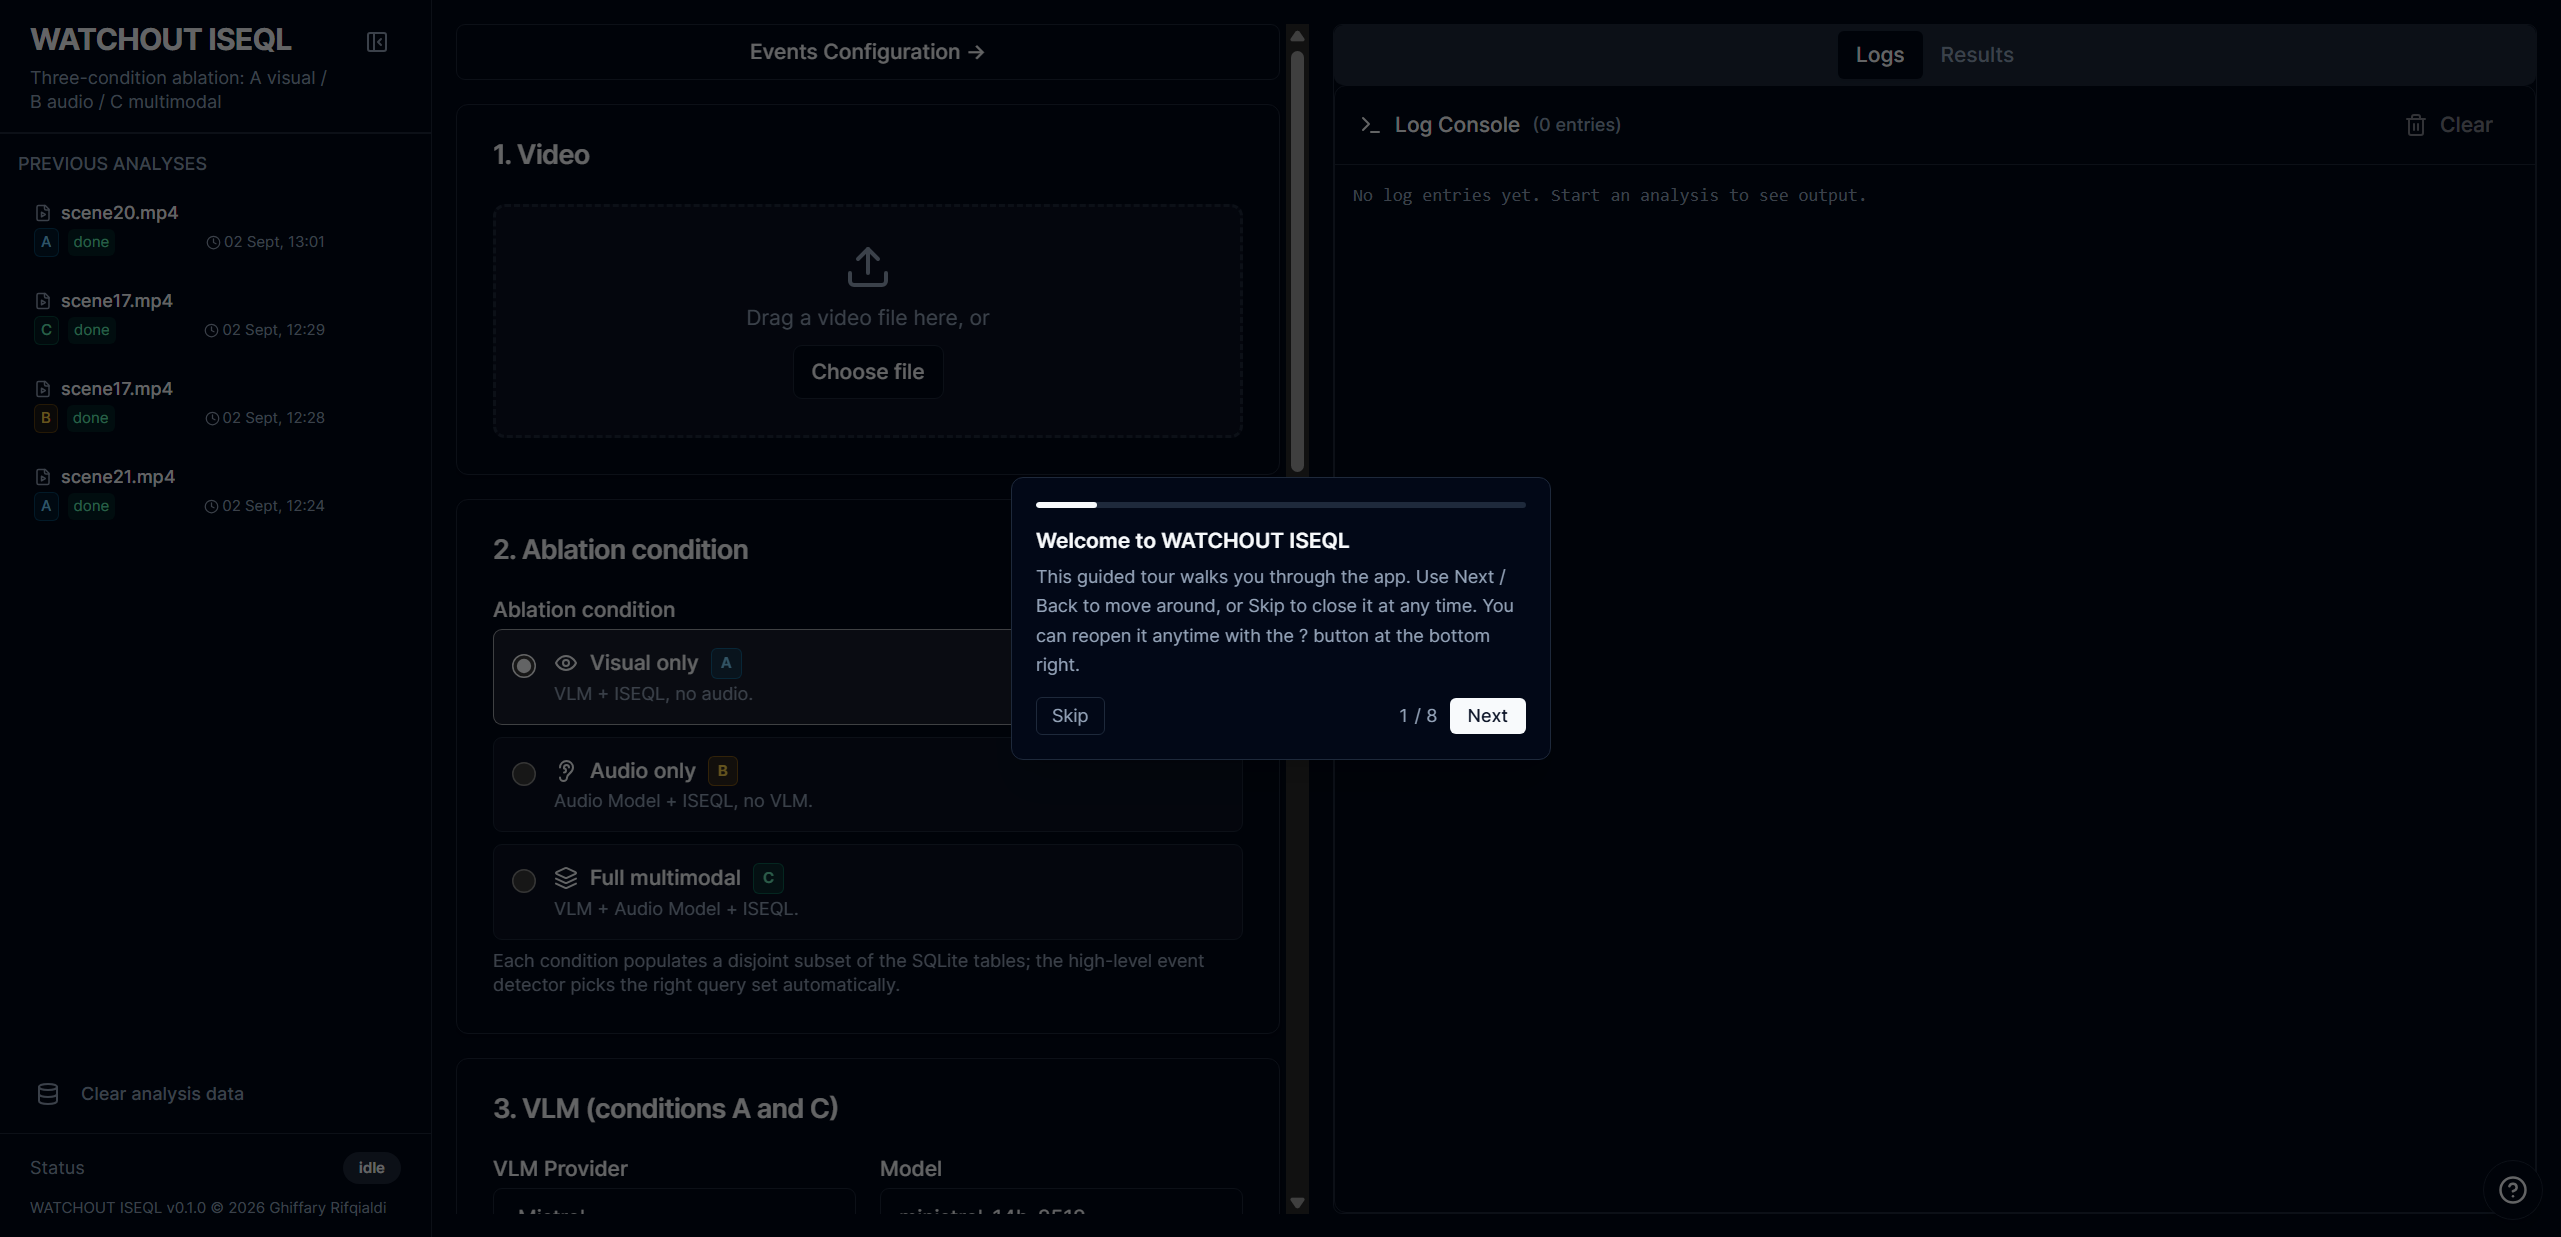
\includegraphics[width=0.92\textwidth]{Figures/appendix/tour01_landing.png}
  \caption{Welcome to WATCHOUT ISEQL: the guided tour walks you through the app.}
\end{figure}

\begin{figure}[H]
  \centering
  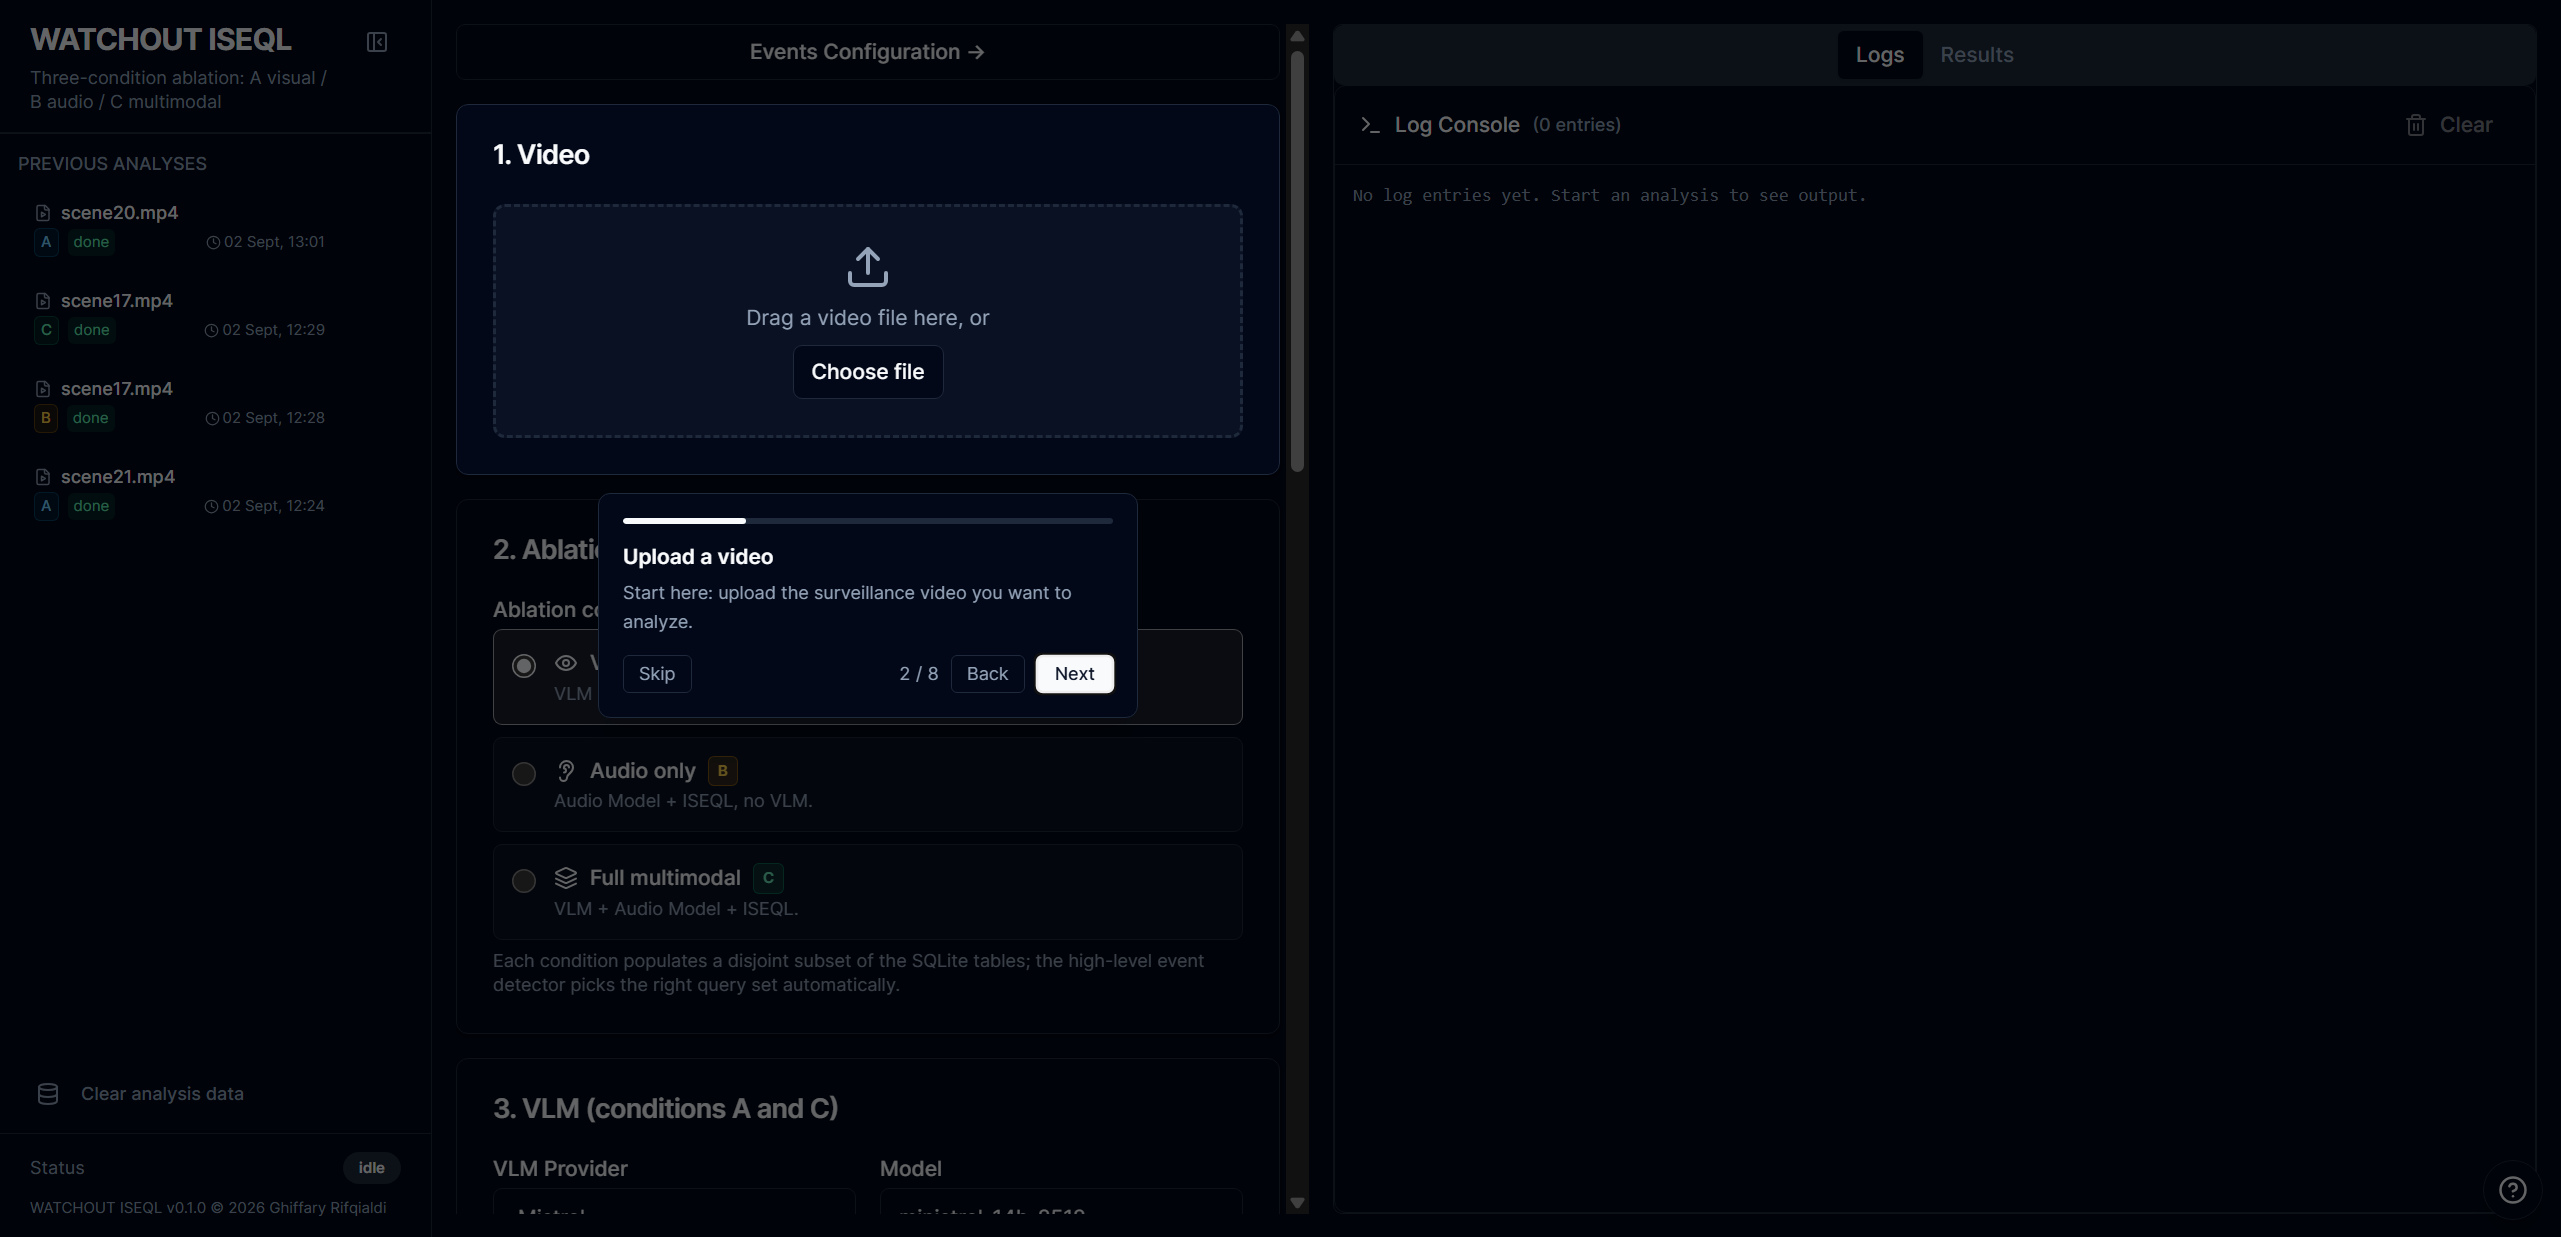
\includegraphics[width=0.92\textwidth]{Figures/appendix/tour02_upload.png}
  \caption{Upload a video: start here, upload the surveillance video you want to analyze.}
\end{figure}

\begin{figure}[H]
  \centering
  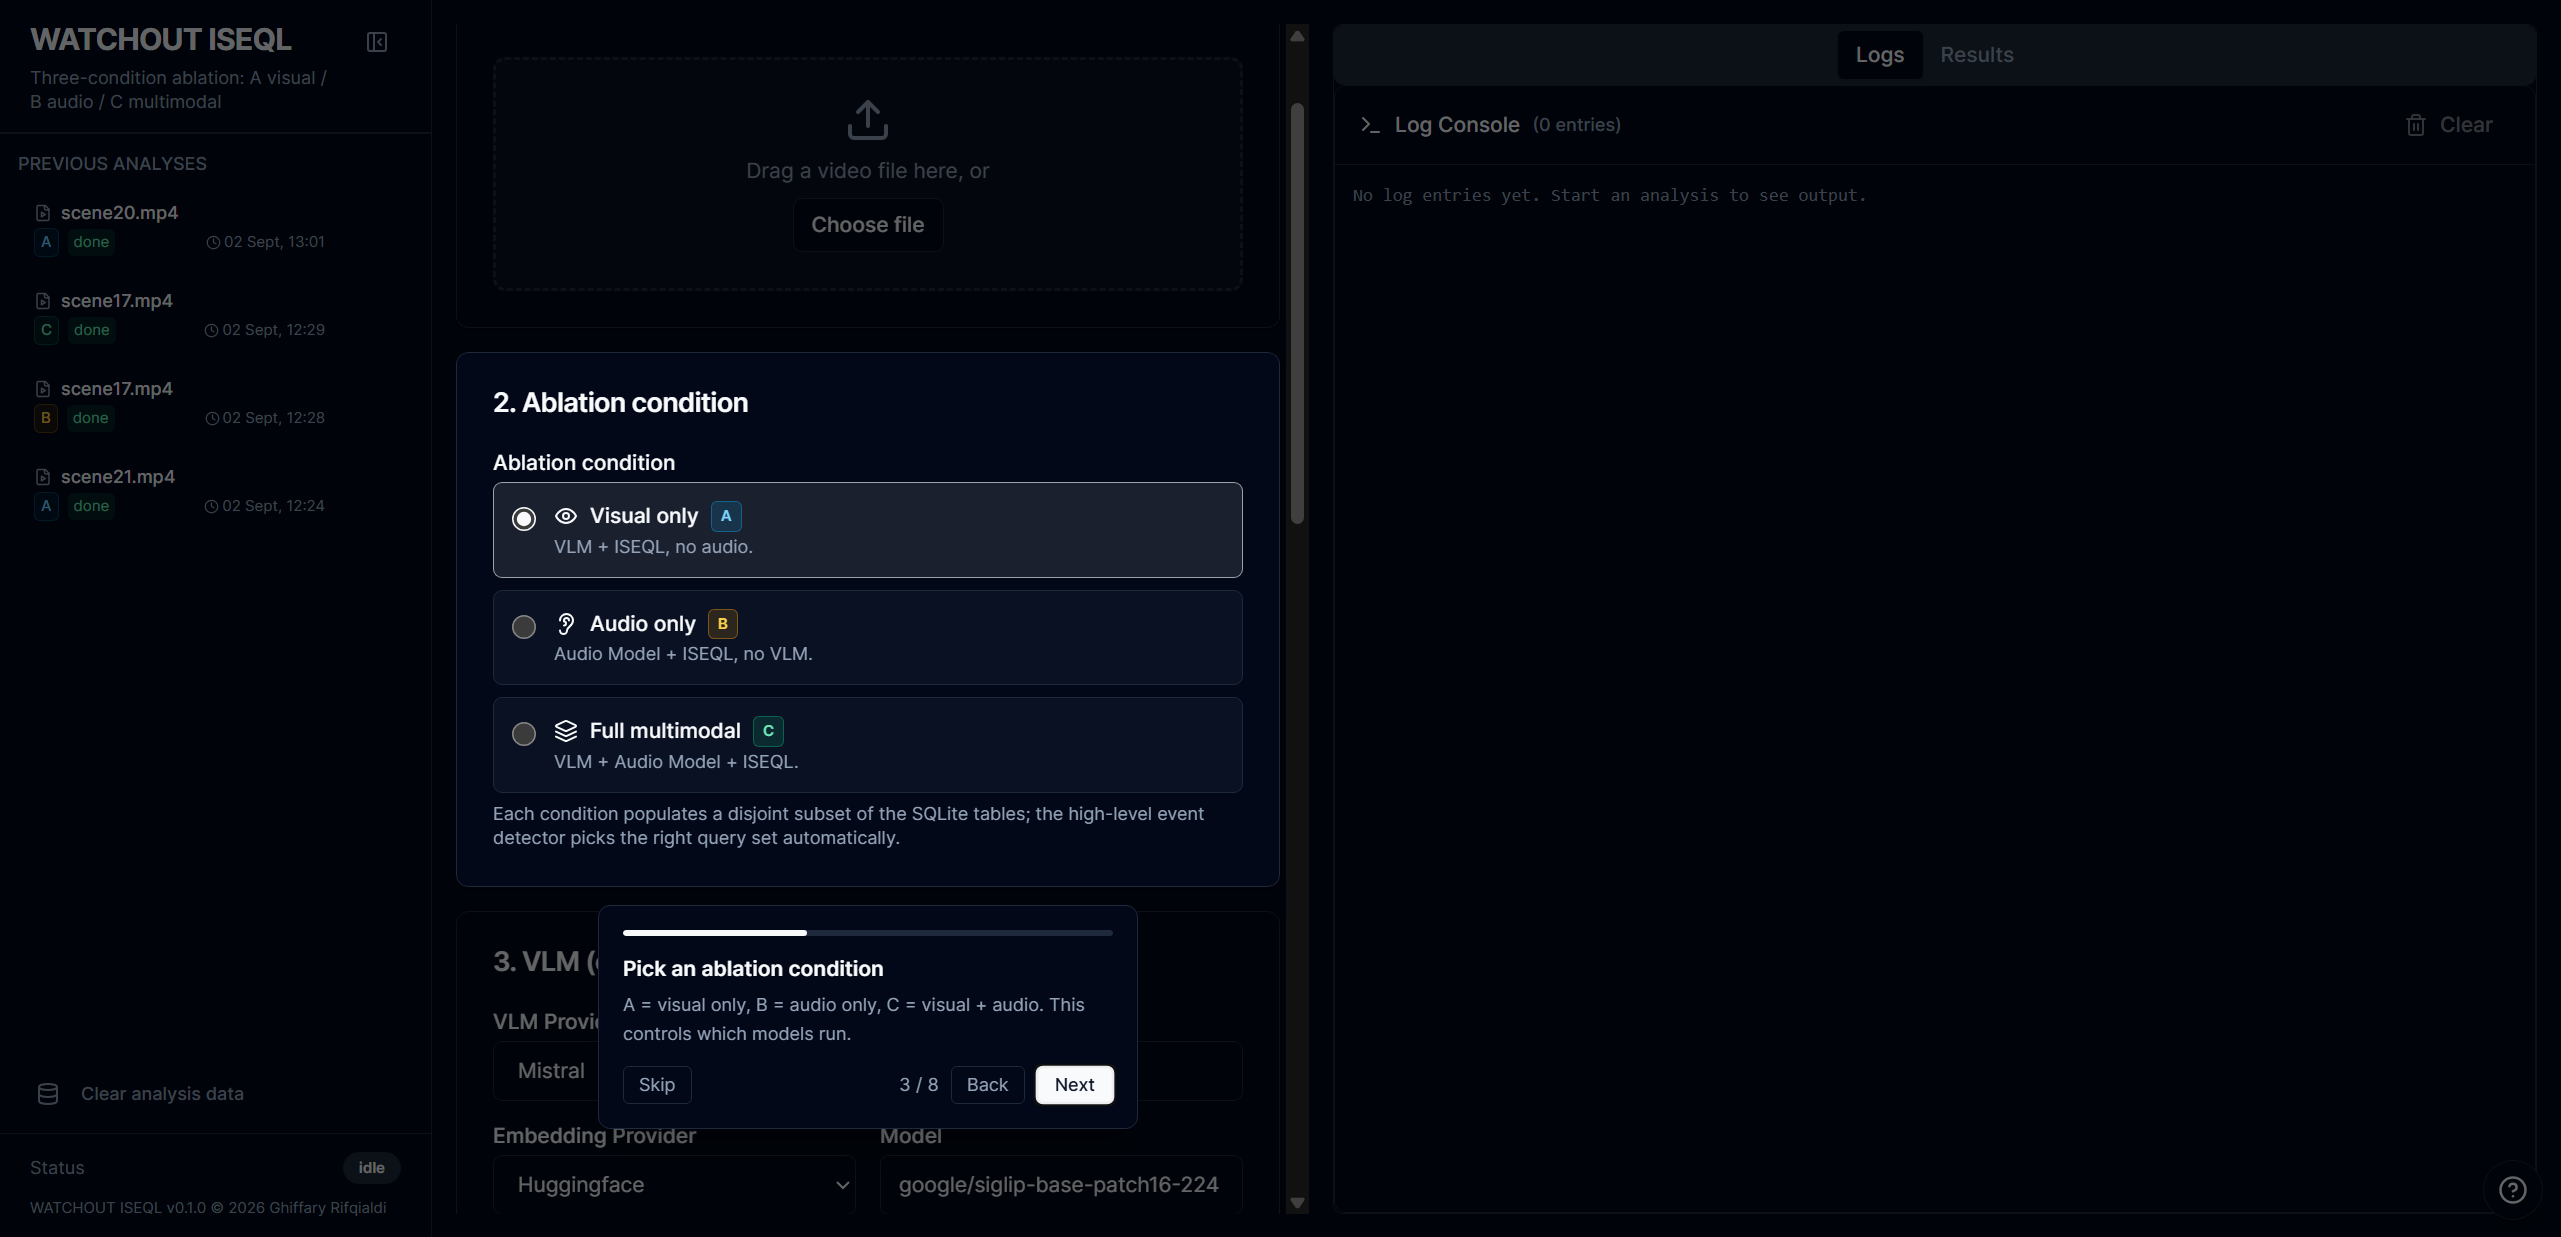
\includegraphics[width=0.92\textwidth]{Figures/appendix/tour03_condition.png}
  \caption{Pick an ablation condition: A = visual only, B = audio only, C = visual + audio.}
\end{figure}

\begin{figure}[H]
  \centering
  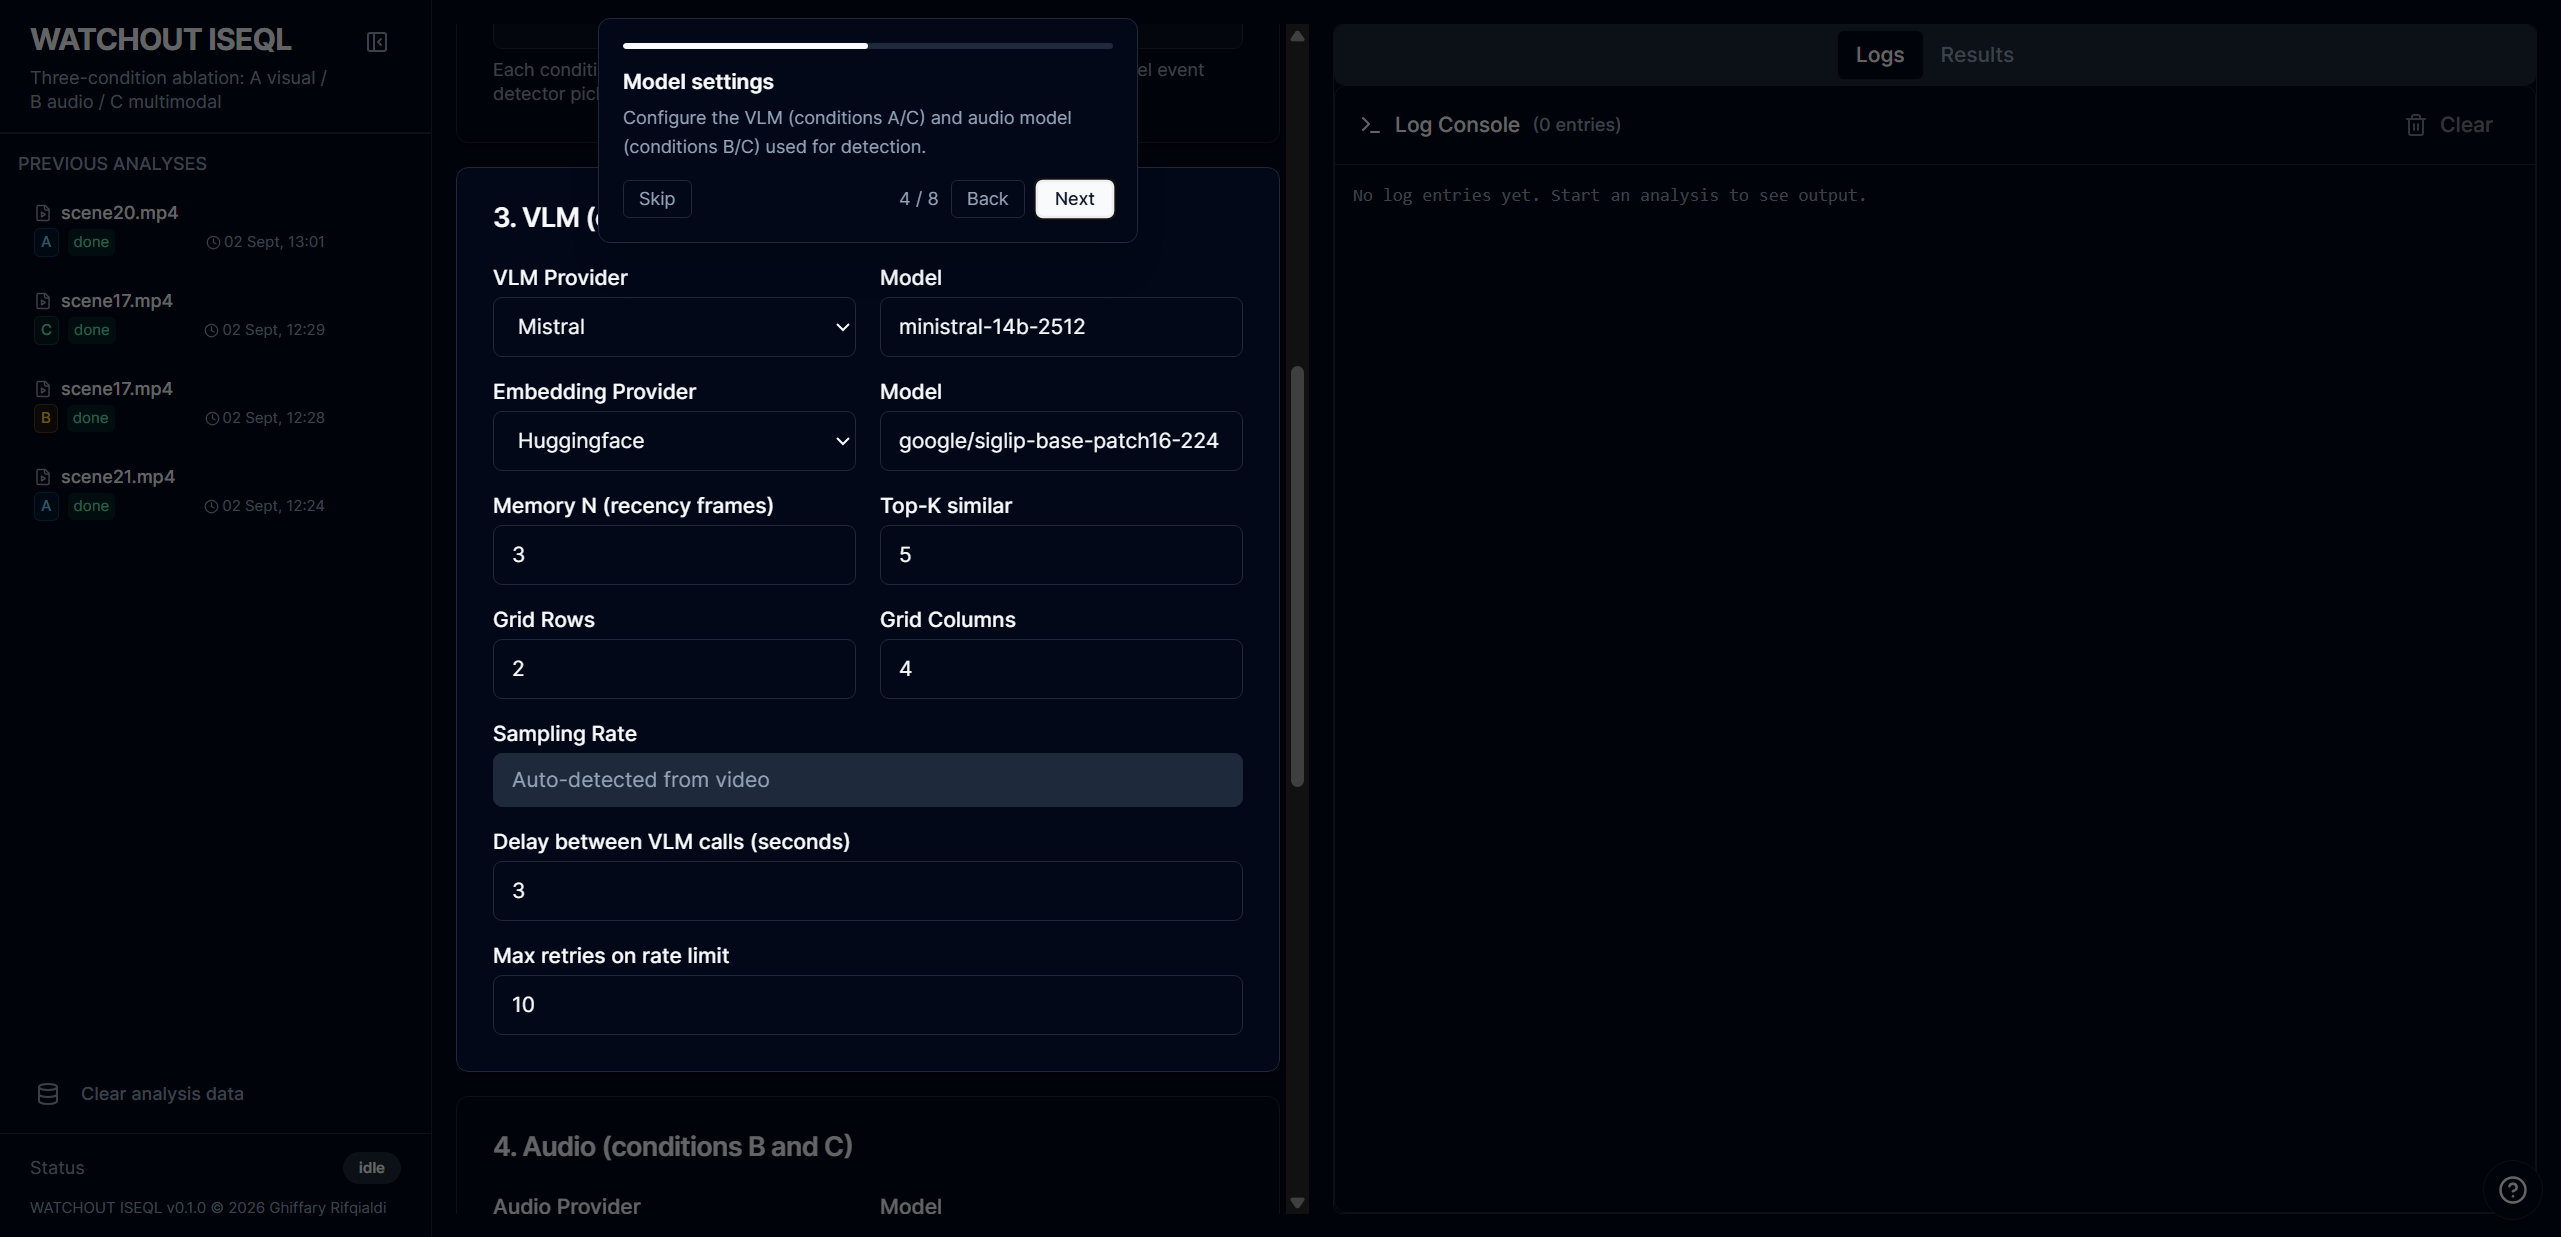
\includegraphics[width=0.92\textwidth]{Figures/appendix/tour04_model.png}
  \caption{Model settings: configure the VLM (conditions A/C) and audio model (conditions B/C).}
\end{figure}

\begin{figure}[H]
  \centering
  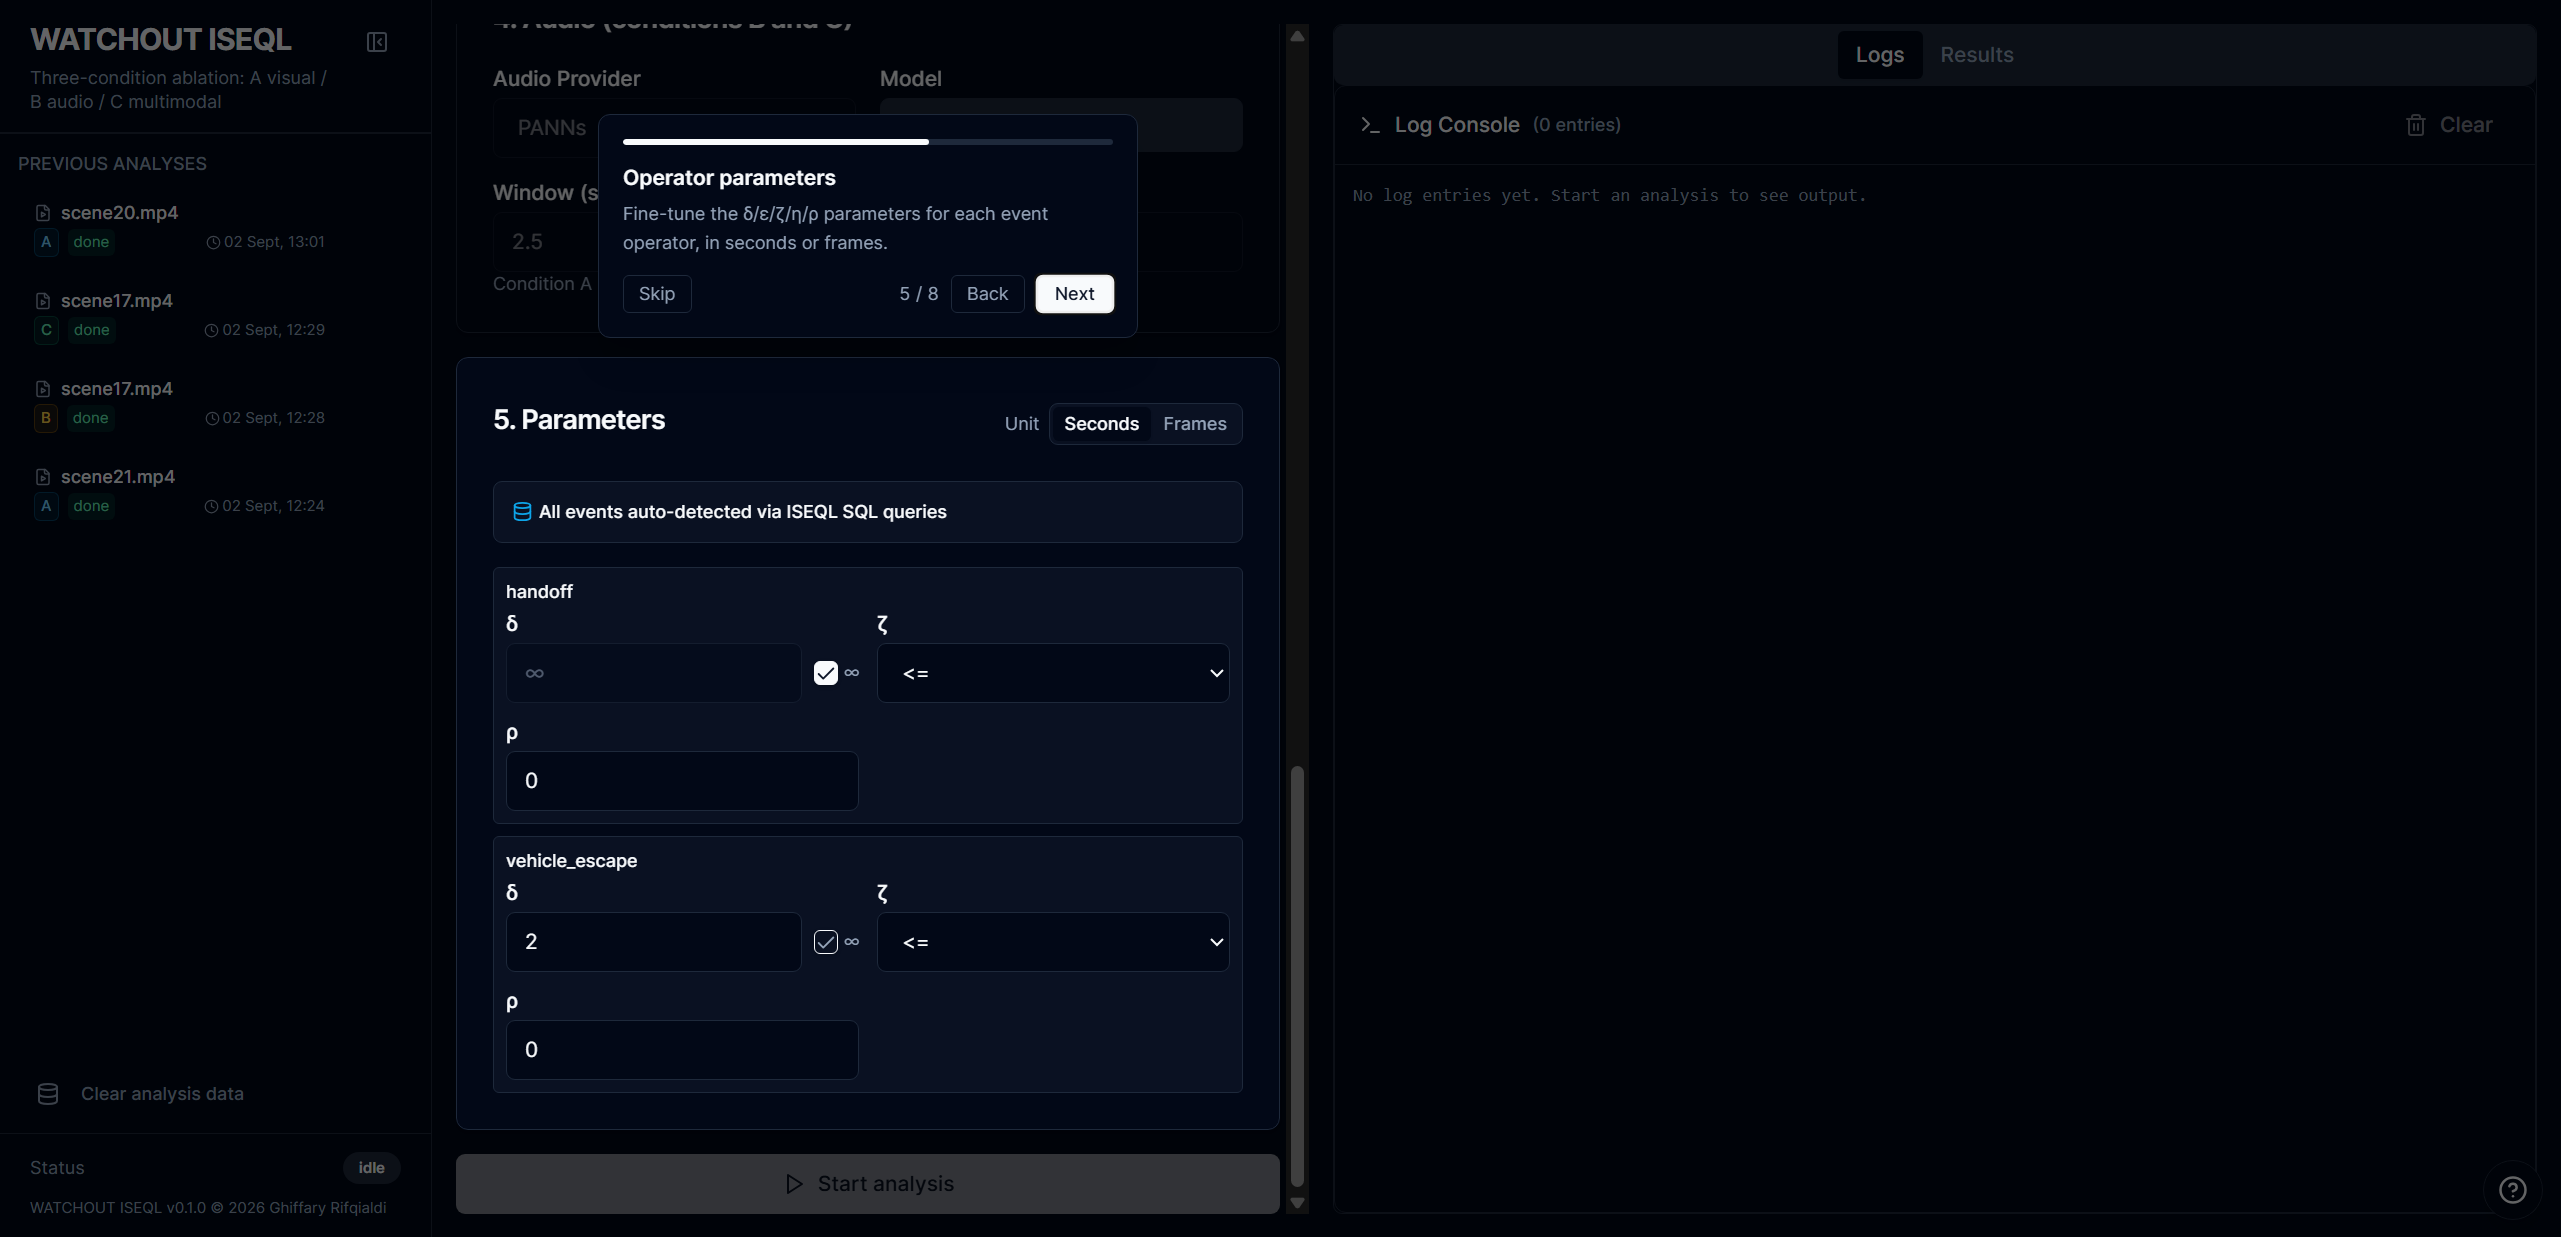
\includegraphics[width=0.92\textwidth]{Figures/appendix/tour05_params.png}
  \caption{Operator parameters: fine-tune the $\delta$, $\epsilon$, $\zeta$, $\eta$, $\rho$ parameters for each event operator.}
\end{figure}

\begin{figure}[H]
  \centering
  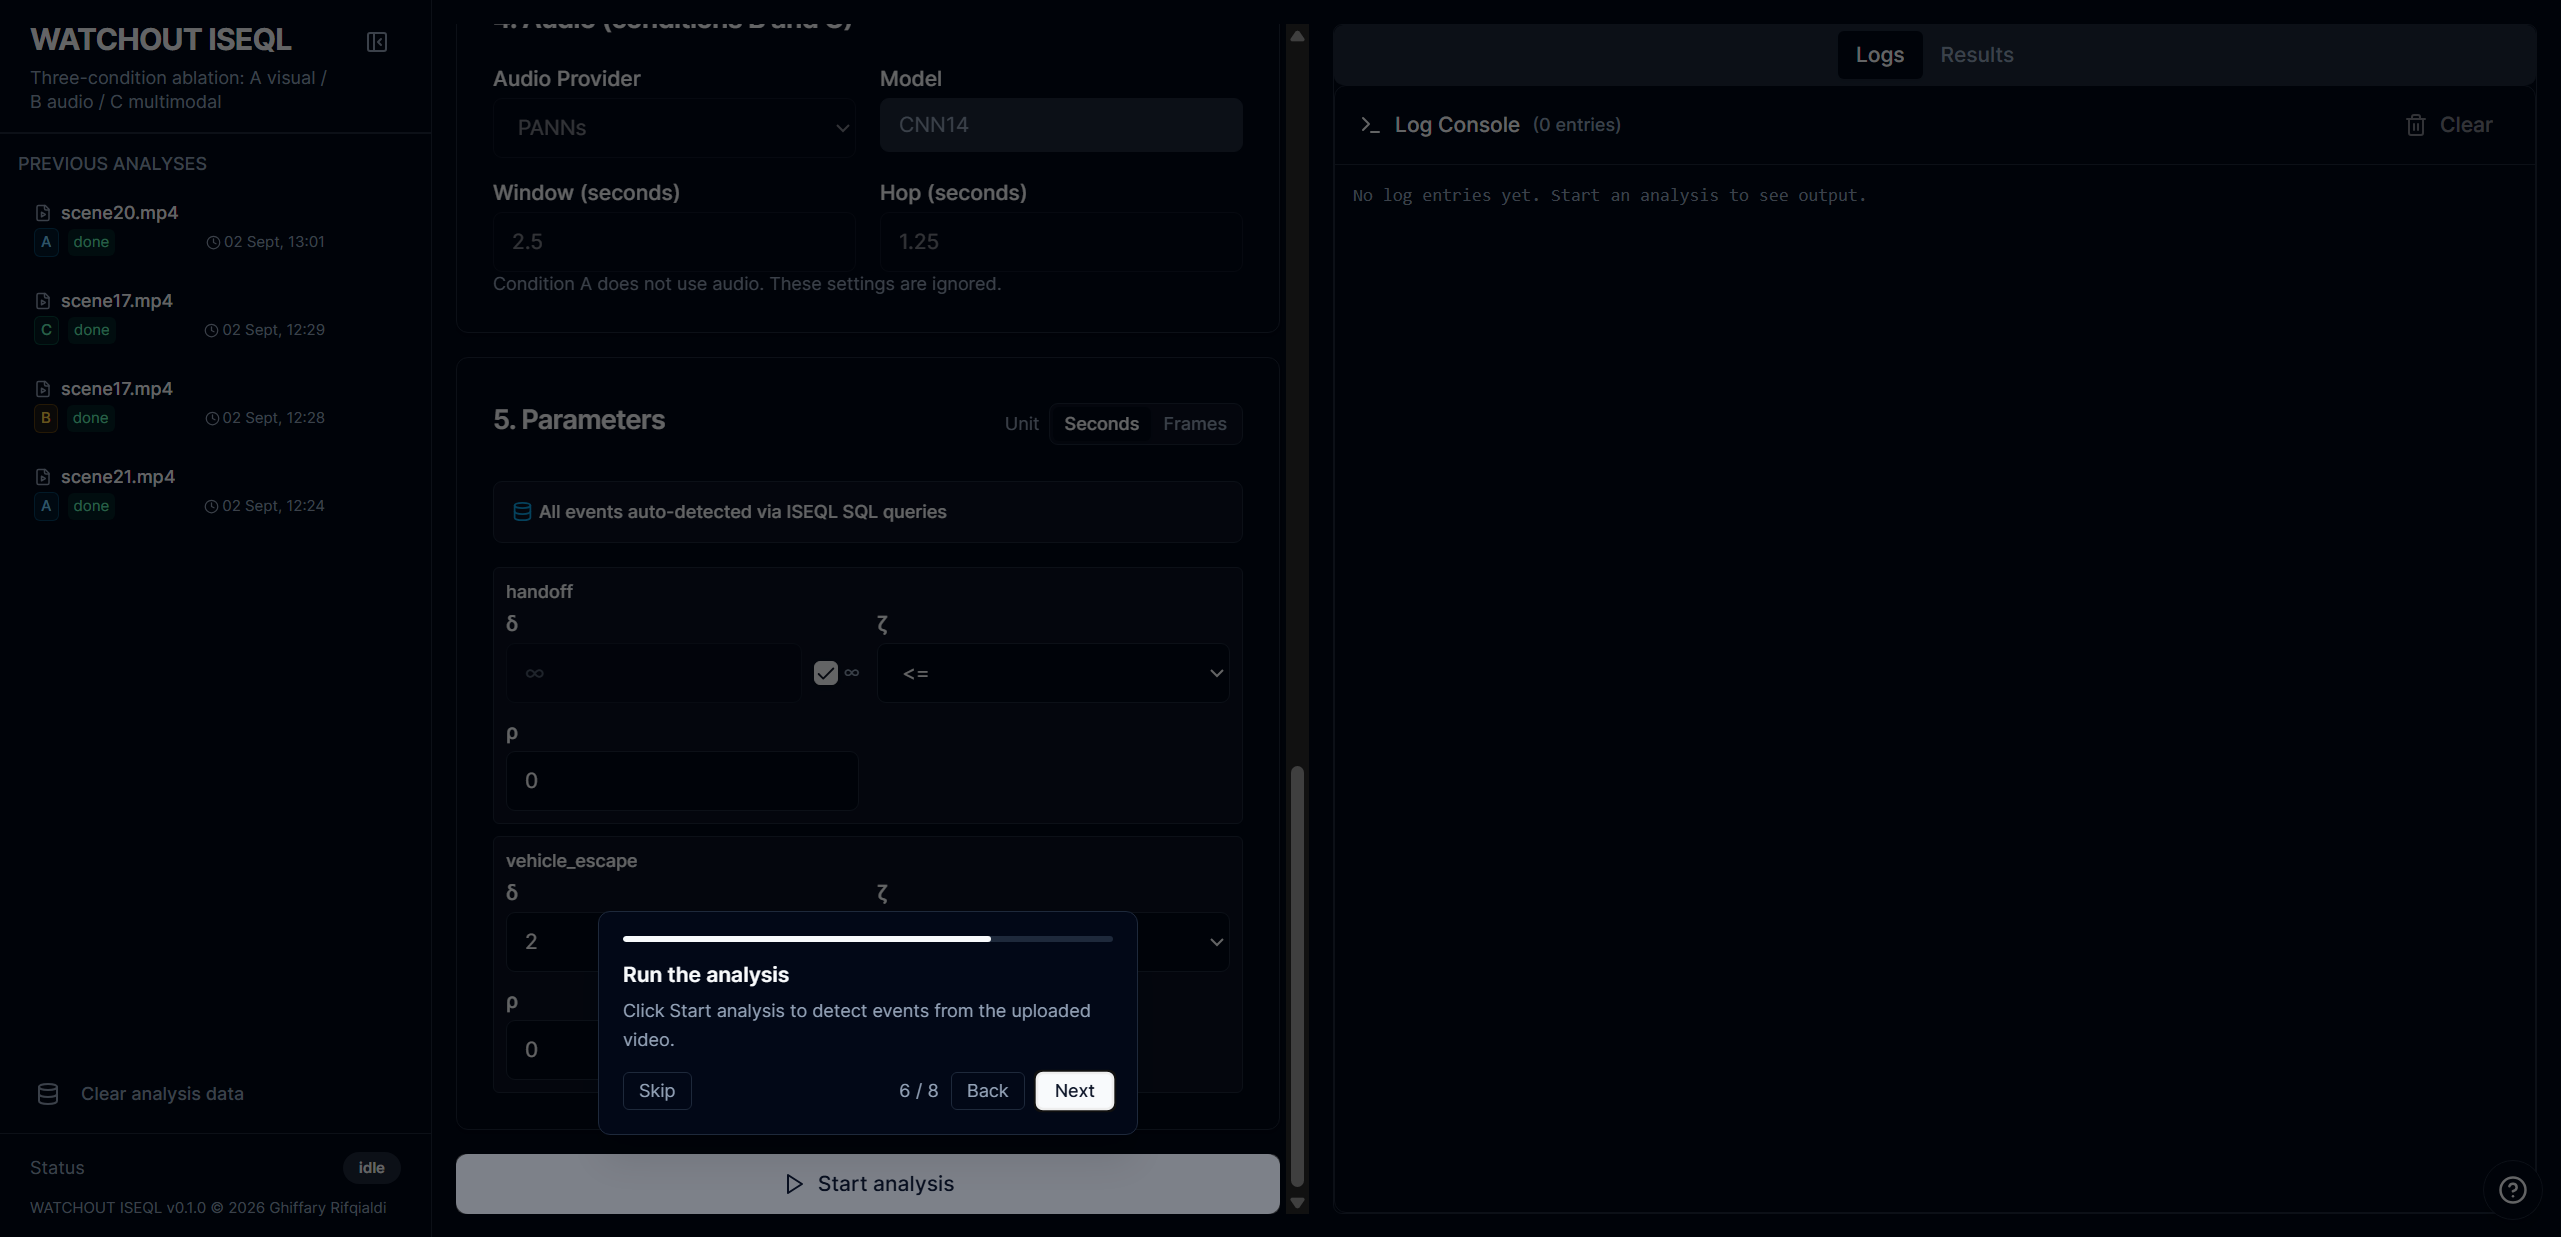
\includegraphics[width=0.92\textwidth]{Figures/appendix/tour06_run.png}
  \caption{Run the analysis: click Start analysis to detect events from the uploaded video.}
\end{figure}

\begin{figure}[H]
  \centering
  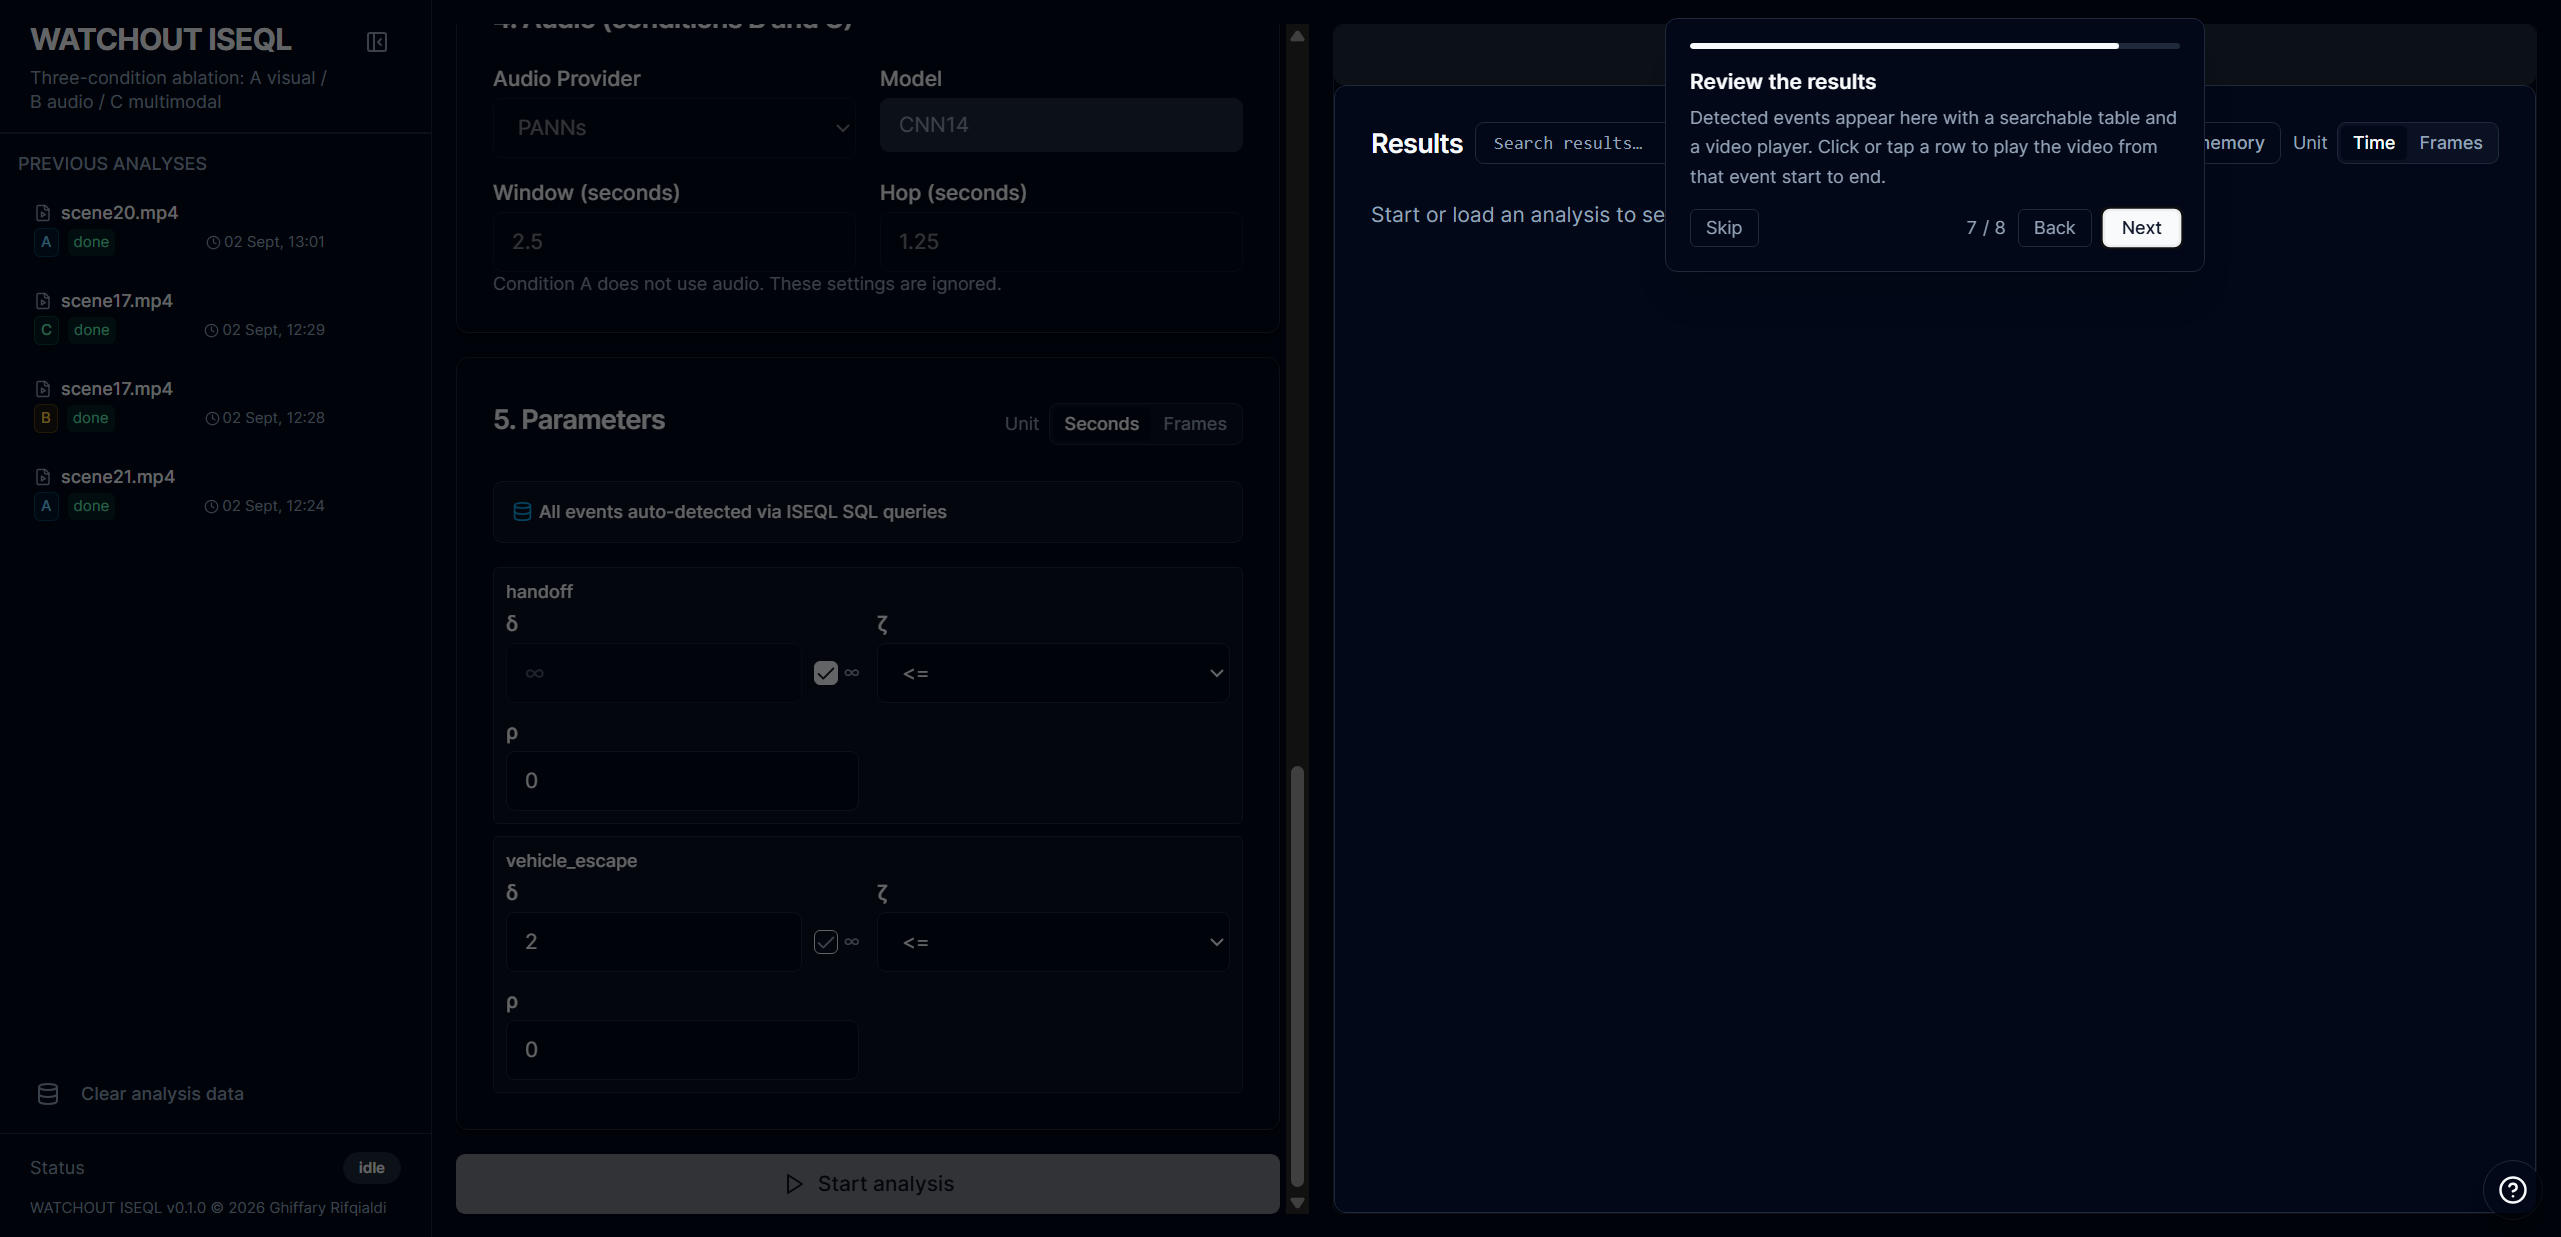
\includegraphics[width=0.92\textwidth]{Figures/appendix/tour07_results.png}
  \caption{Review the results: detected events appear in a searchable table with a video player.}
\end{figure}

\begin{figure}[H]
  \centering
  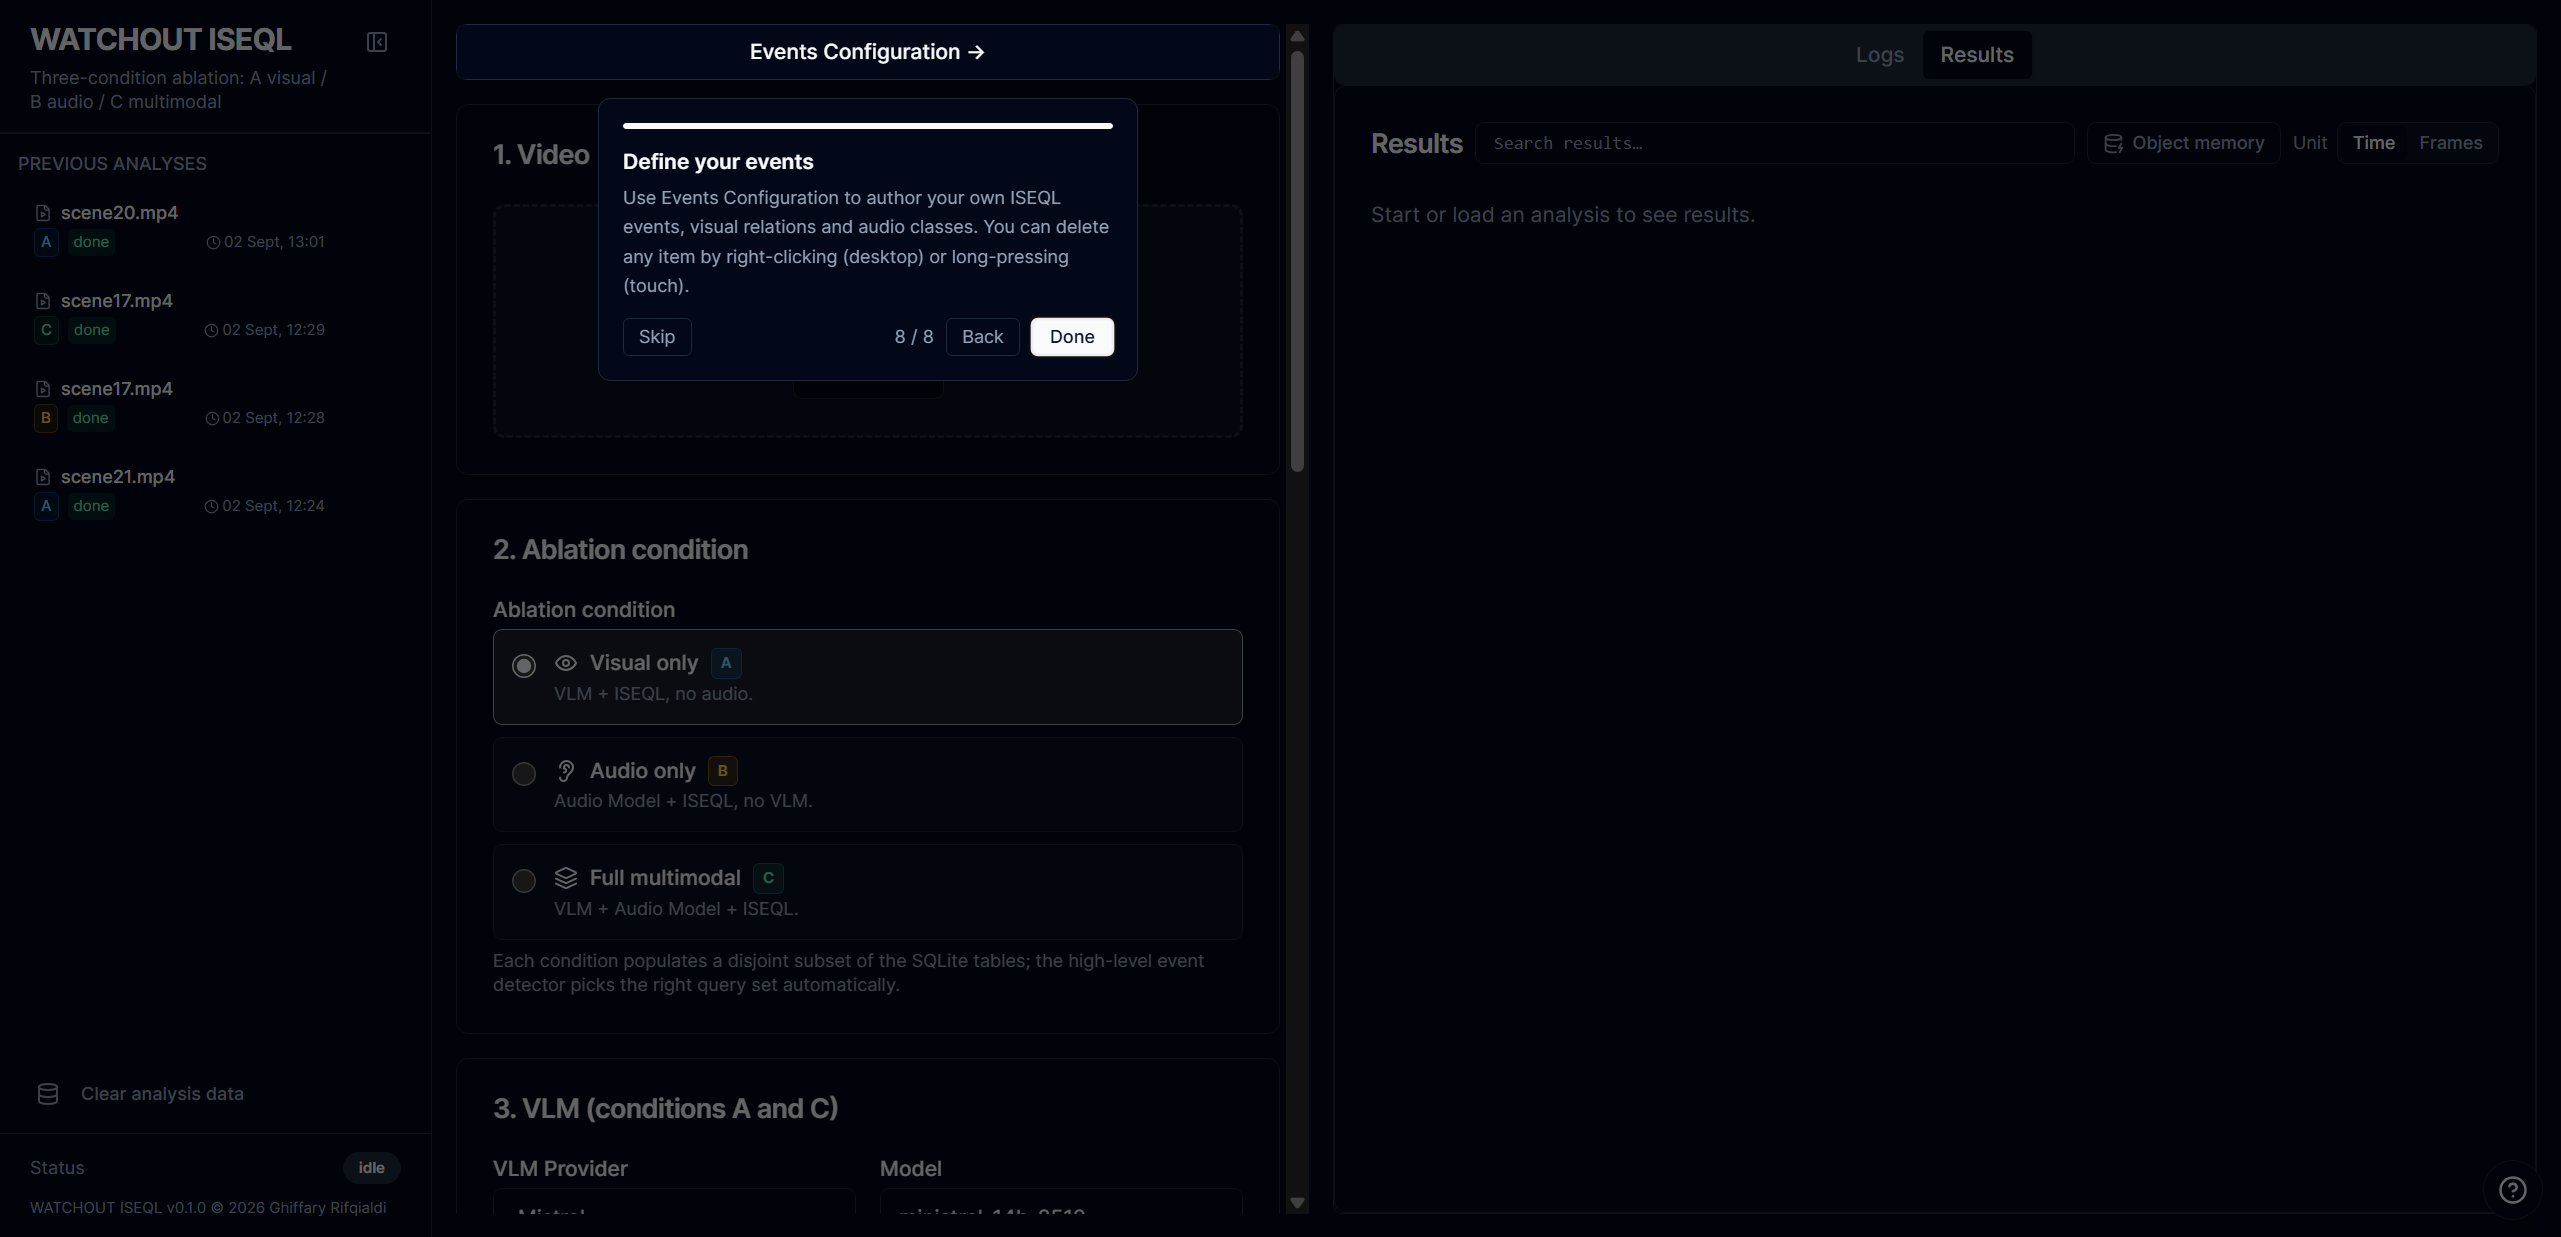
\includegraphics[width=0.92\textwidth]{Figures/appendix/tour08_define_events.png}
  \caption{Define your events: use Events Configuration to author ISEQL events, visual relations and audio classes.}
\end{figure}

\section{Event Configuration}

Events, visual relations, and audio classes are all user-configurable through the web interface. The following figures show the predicates (visual relations and audio classes) and the event authoring flow.

\begin{figure}[H]
  \centering
  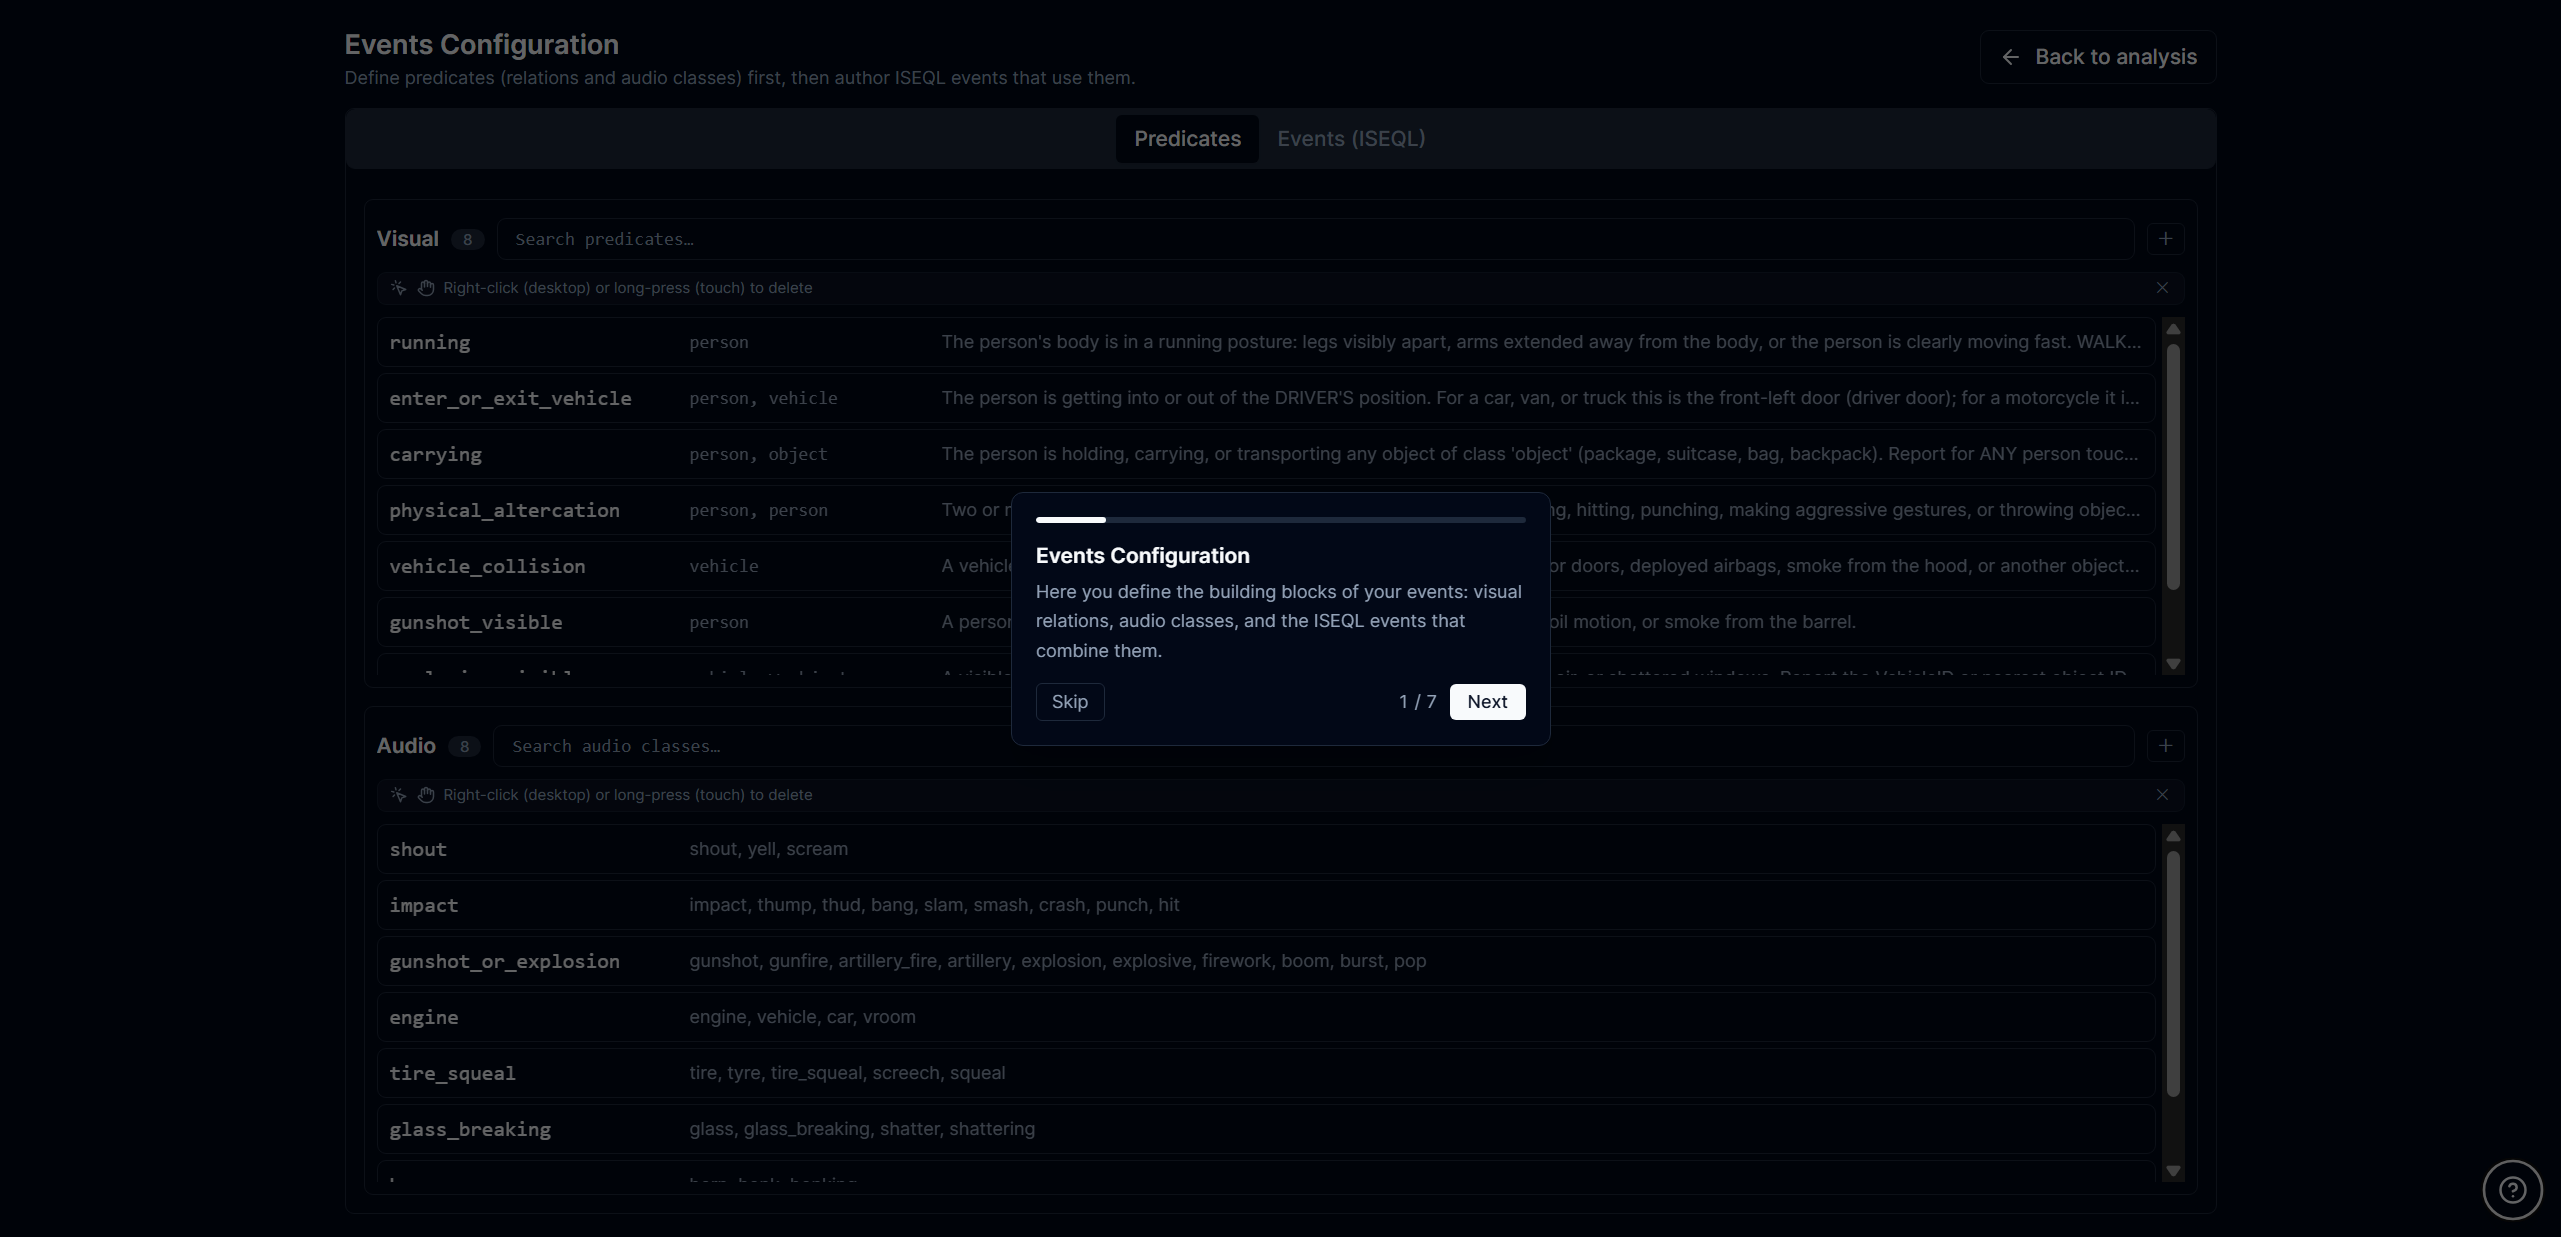
\includegraphics[width=0.92\textwidth]{Figures/appendix/cfg01_predicates.png}
  \caption{Event Configuration: define the building blocks of your events.}
\end{figure}

\begin{figure}[H]
  \centering
  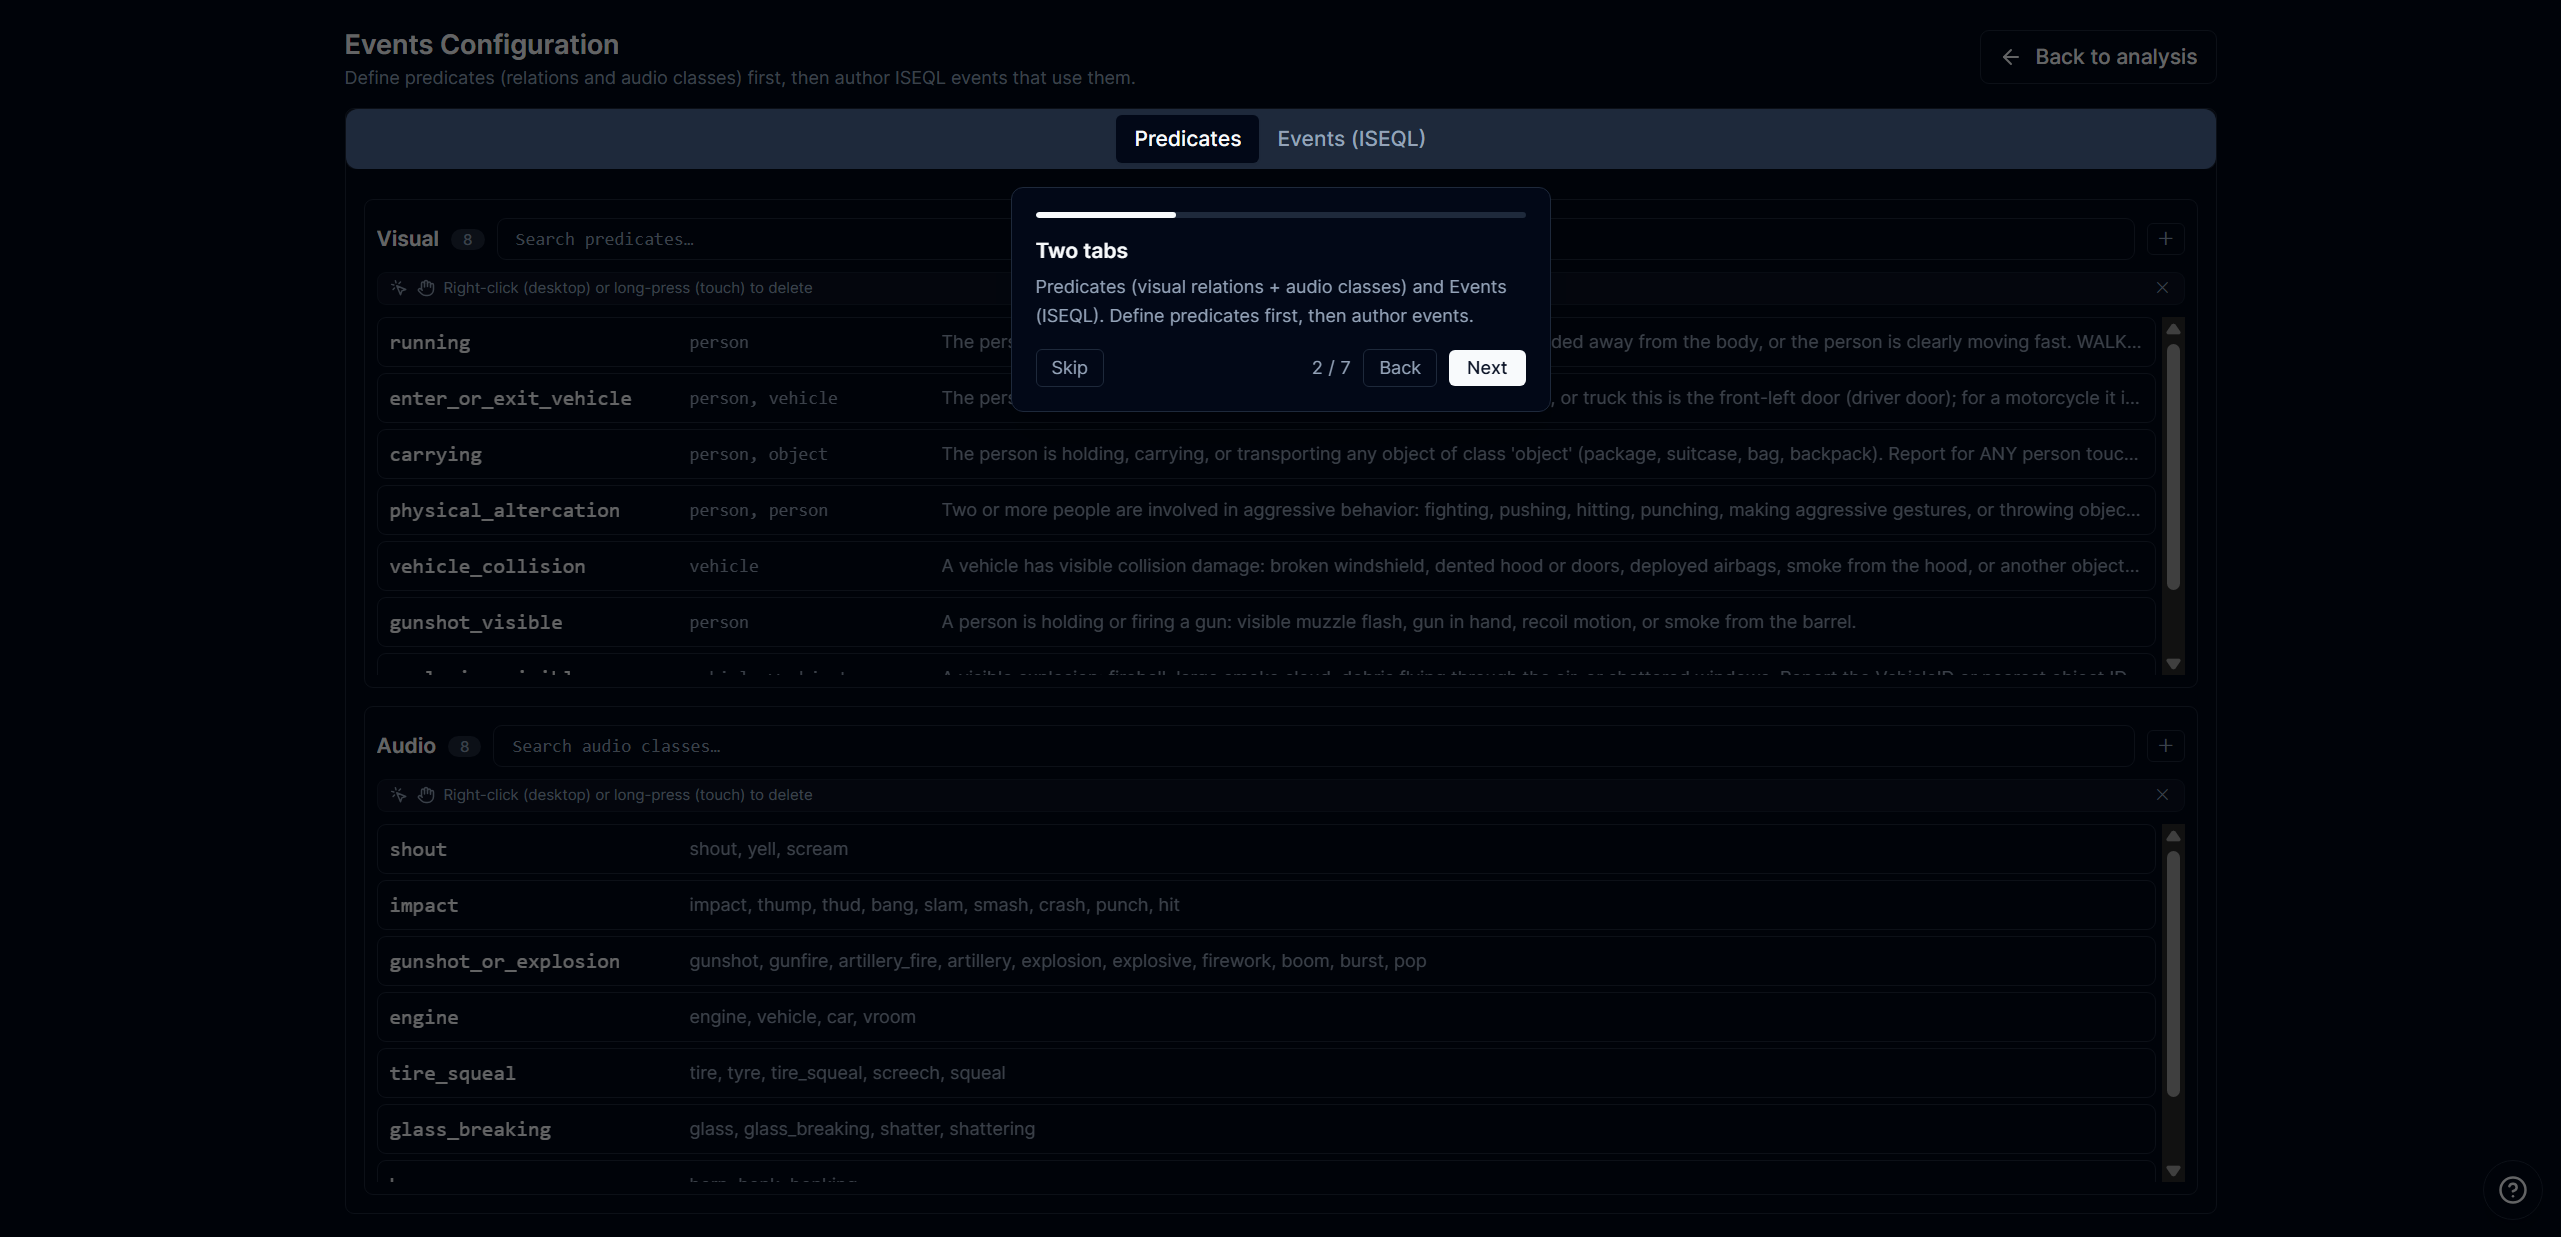
\includegraphics[width=0.92\textwidth]{Figures/appendix/cfg02_predicates_tabs.png}
  \caption{Two tabs: Predicates (visual relations + audio classes) and Events (ISEQL).}
\end{figure}

\begin{figure}[H]
  \centering
  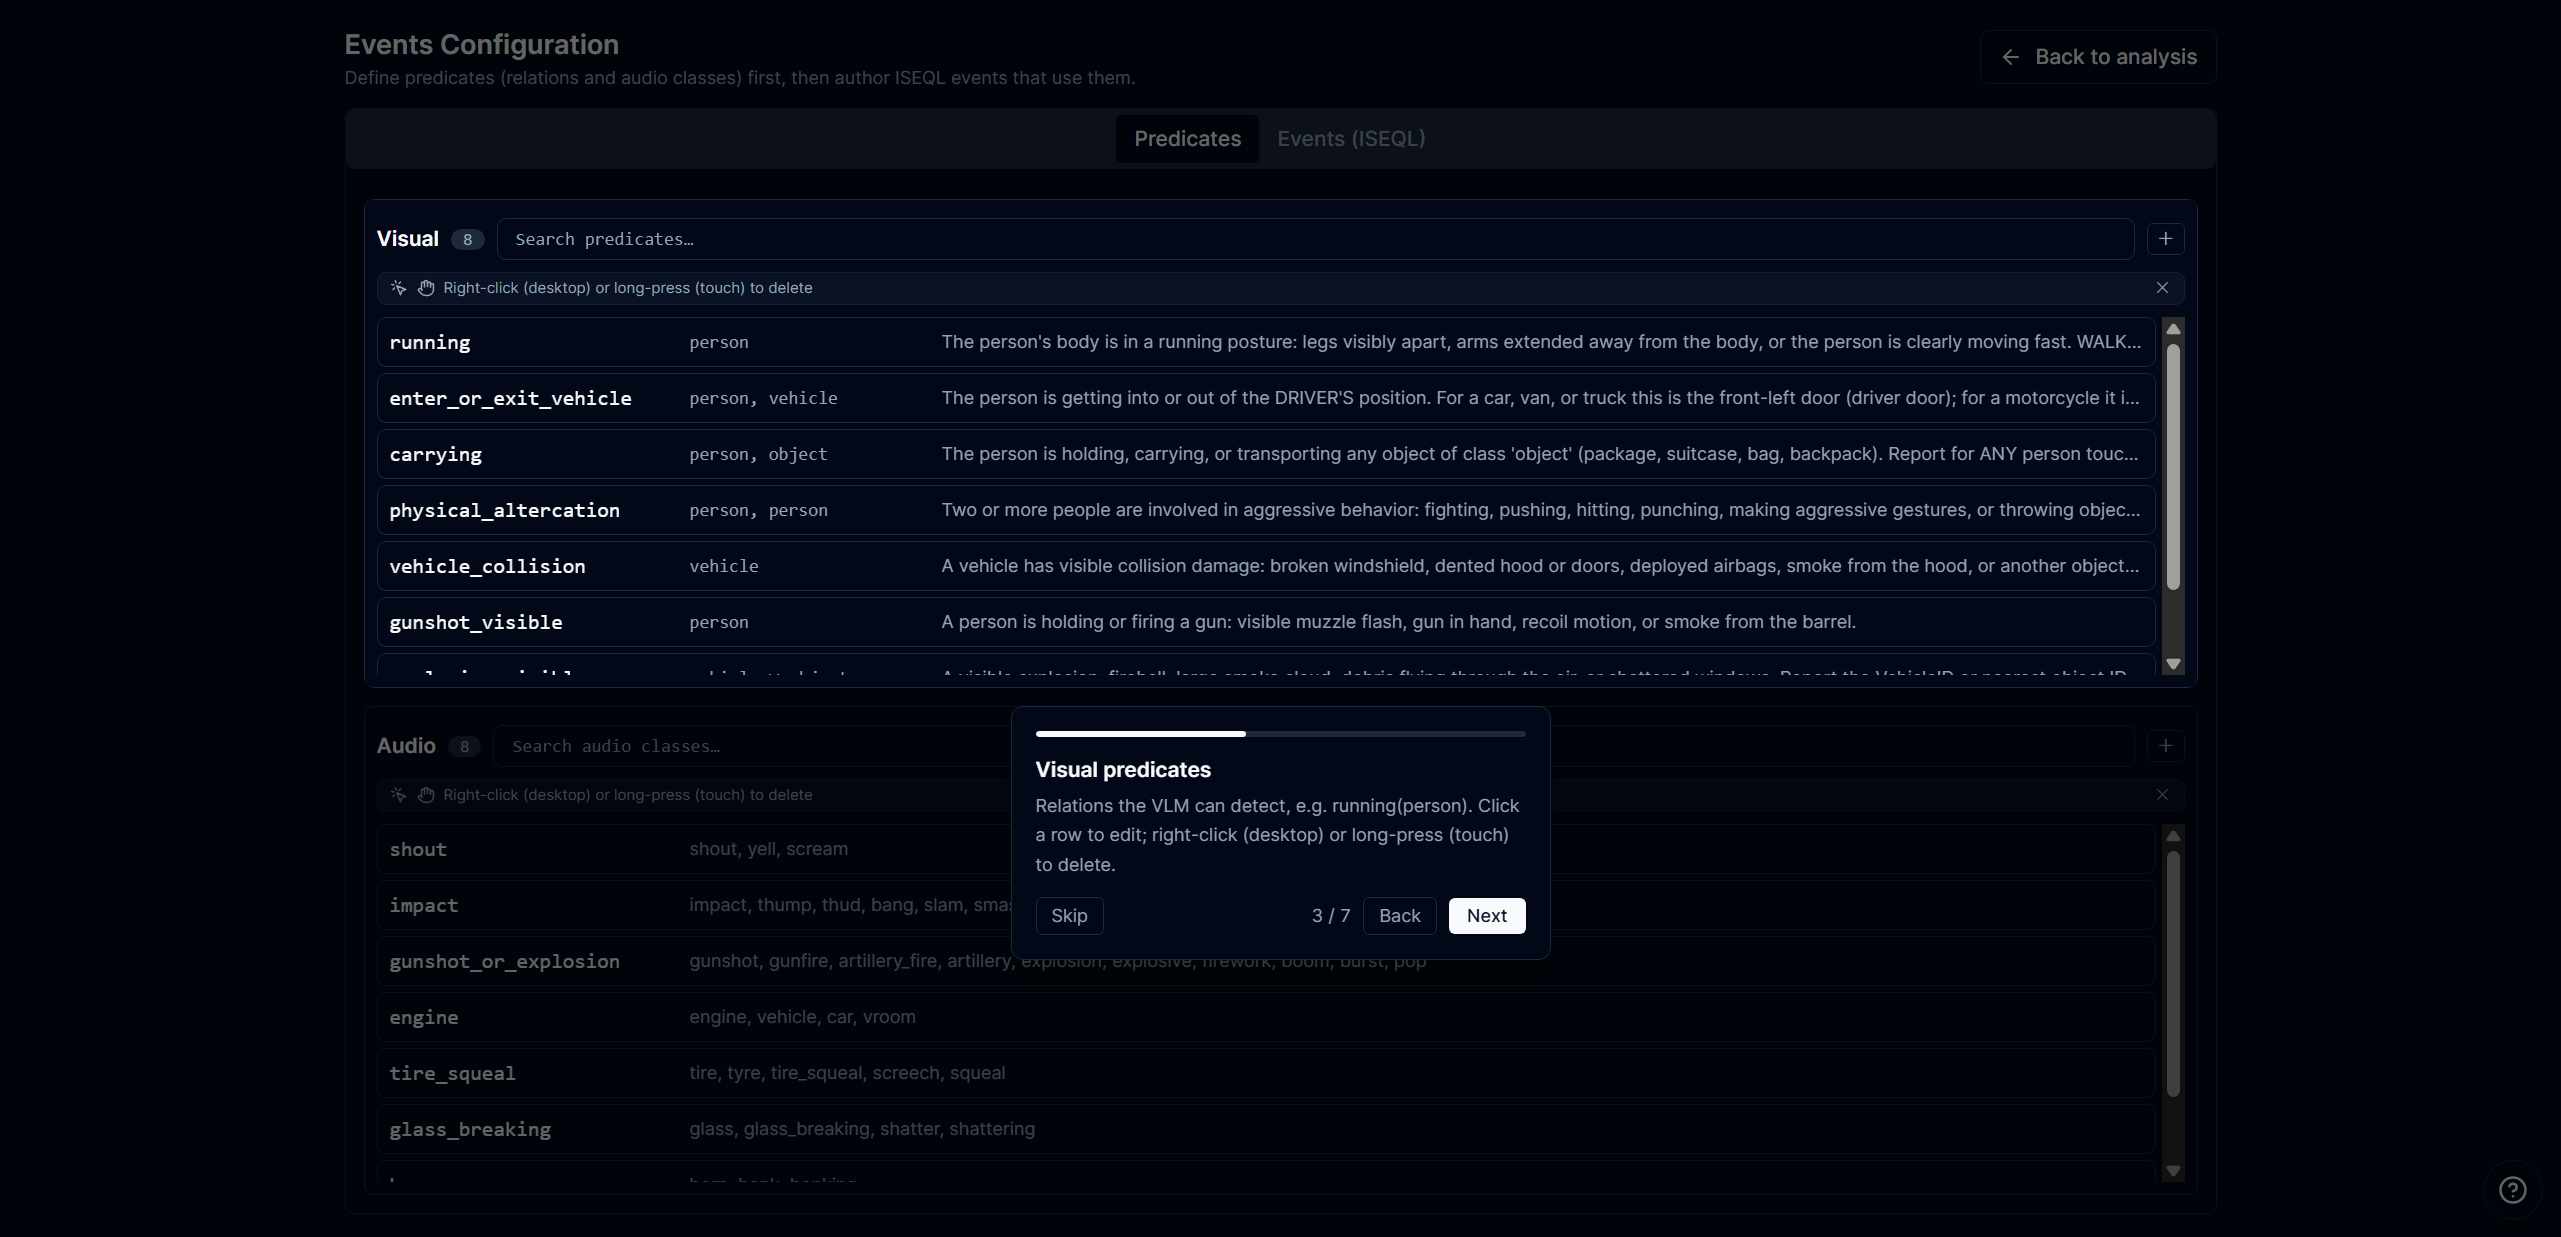
\includegraphics[width=0.92\textwidth]{Figures/appendix/cfg03_visual.png}
  \caption{Visual predicates: relations the VLM can detect, e.g. running(person).}
\end{figure}

\begin{figure}[H]
  \centering
  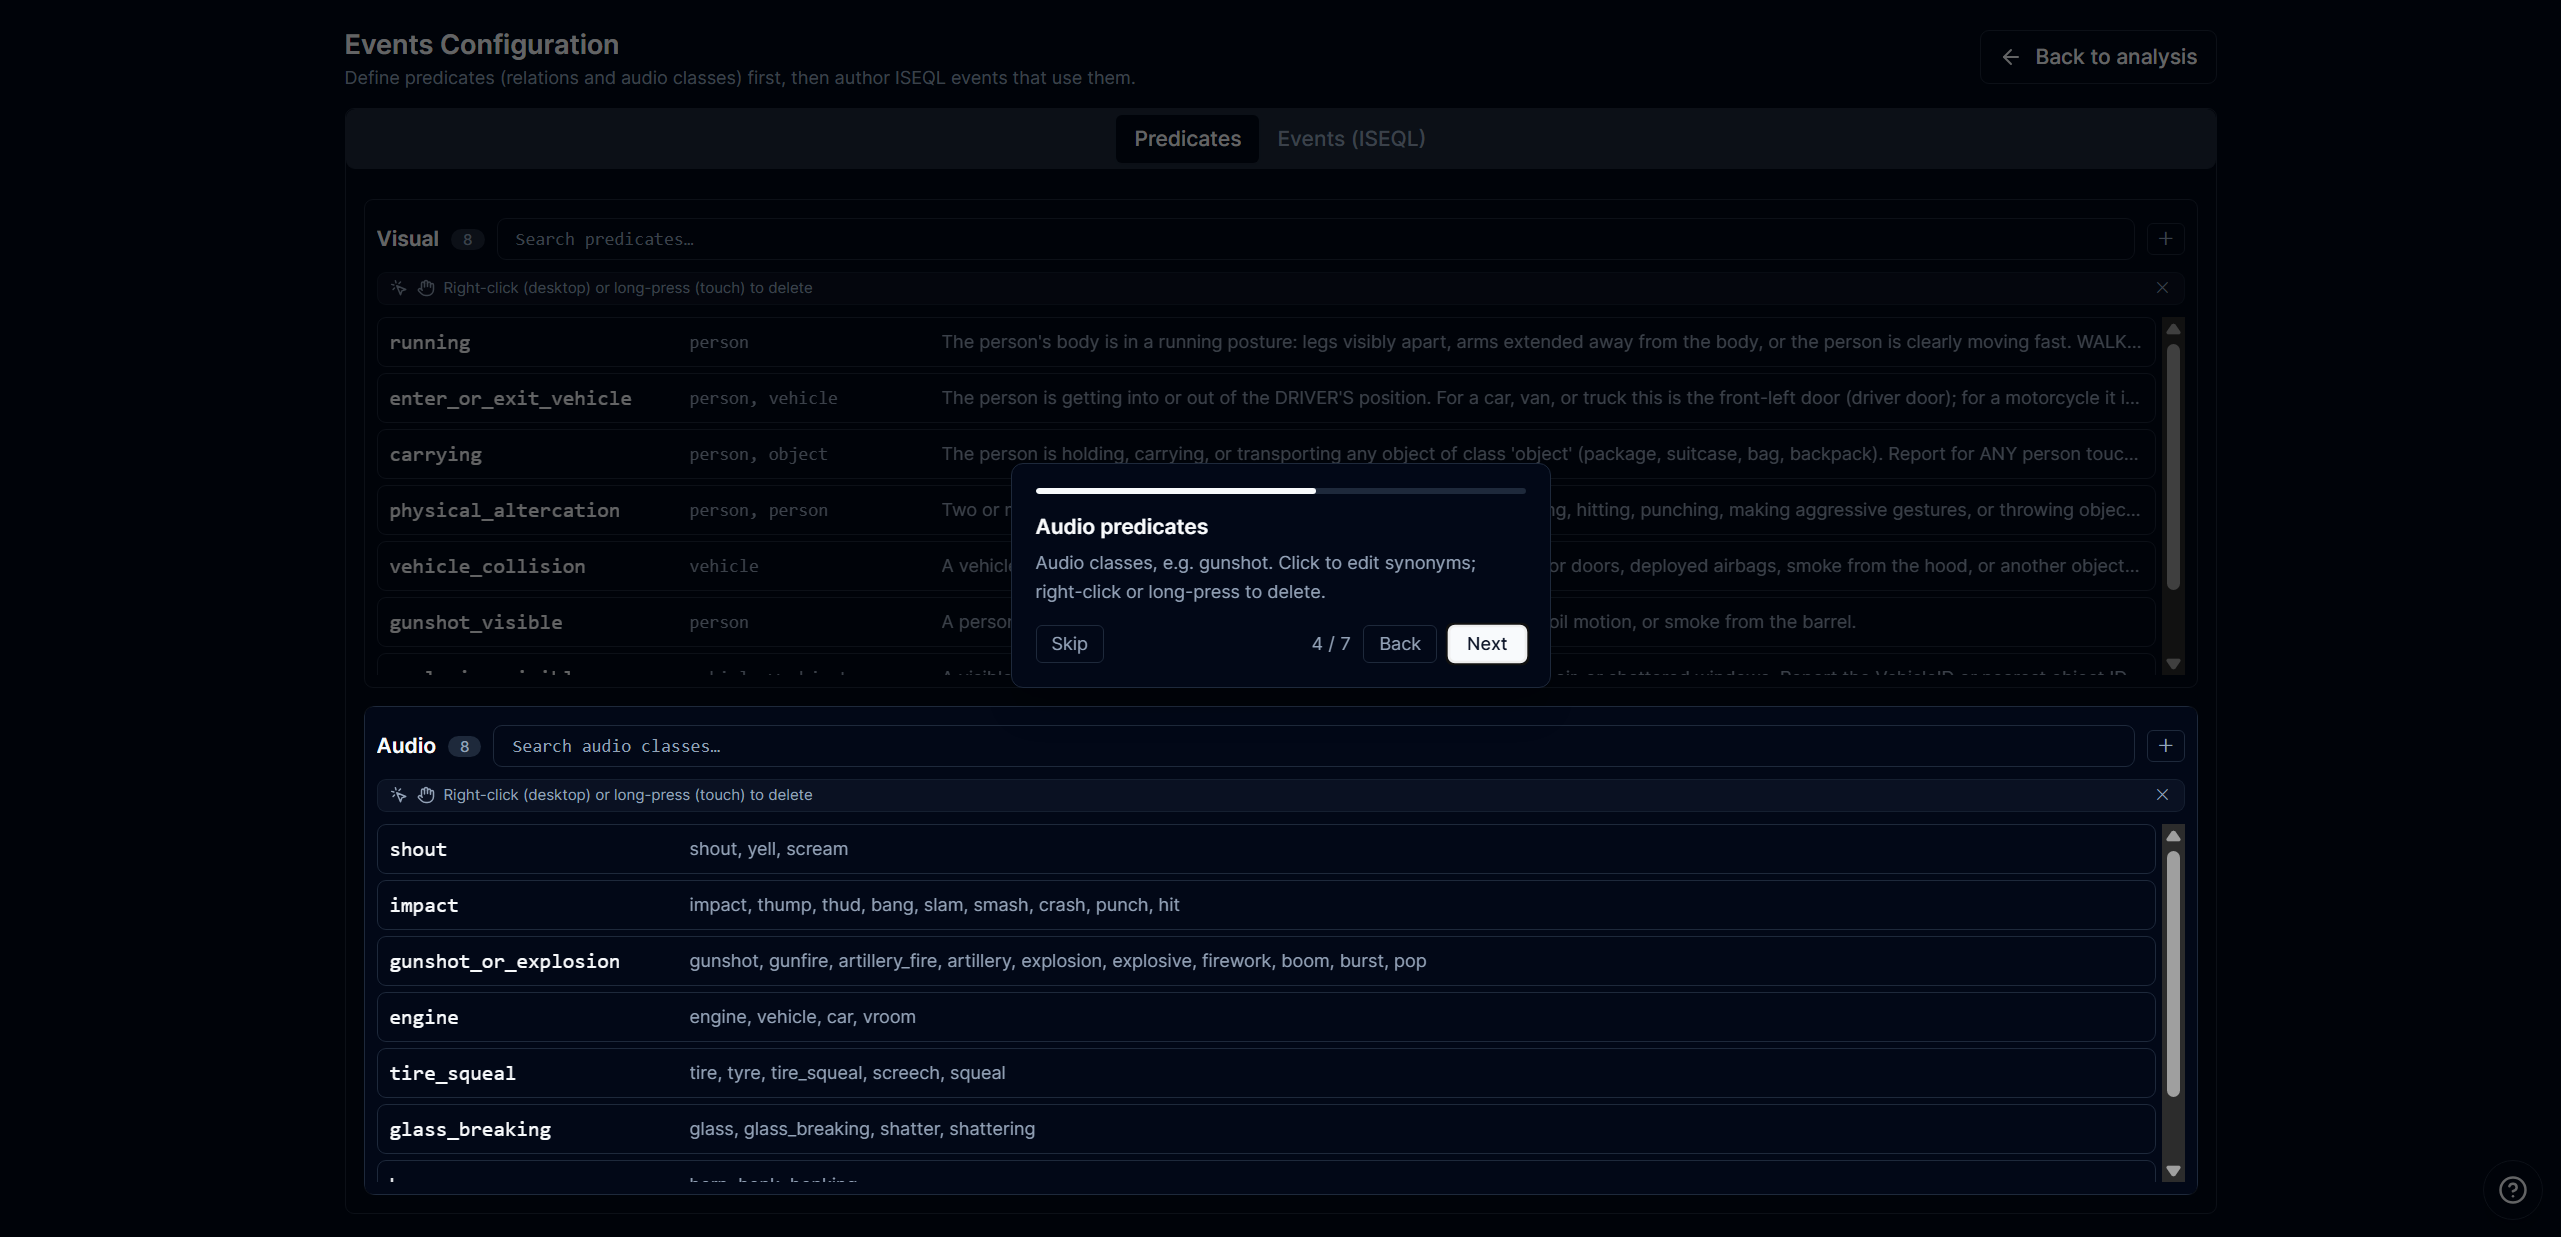
\includegraphics[width=0.92\textwidth]{Figures/appendix/cfg04_audio.png}
  \caption{Audio predicates: audio classes, e.g. gunshot.}
\end{figure}

\begin{figure}[H]
  \centering
  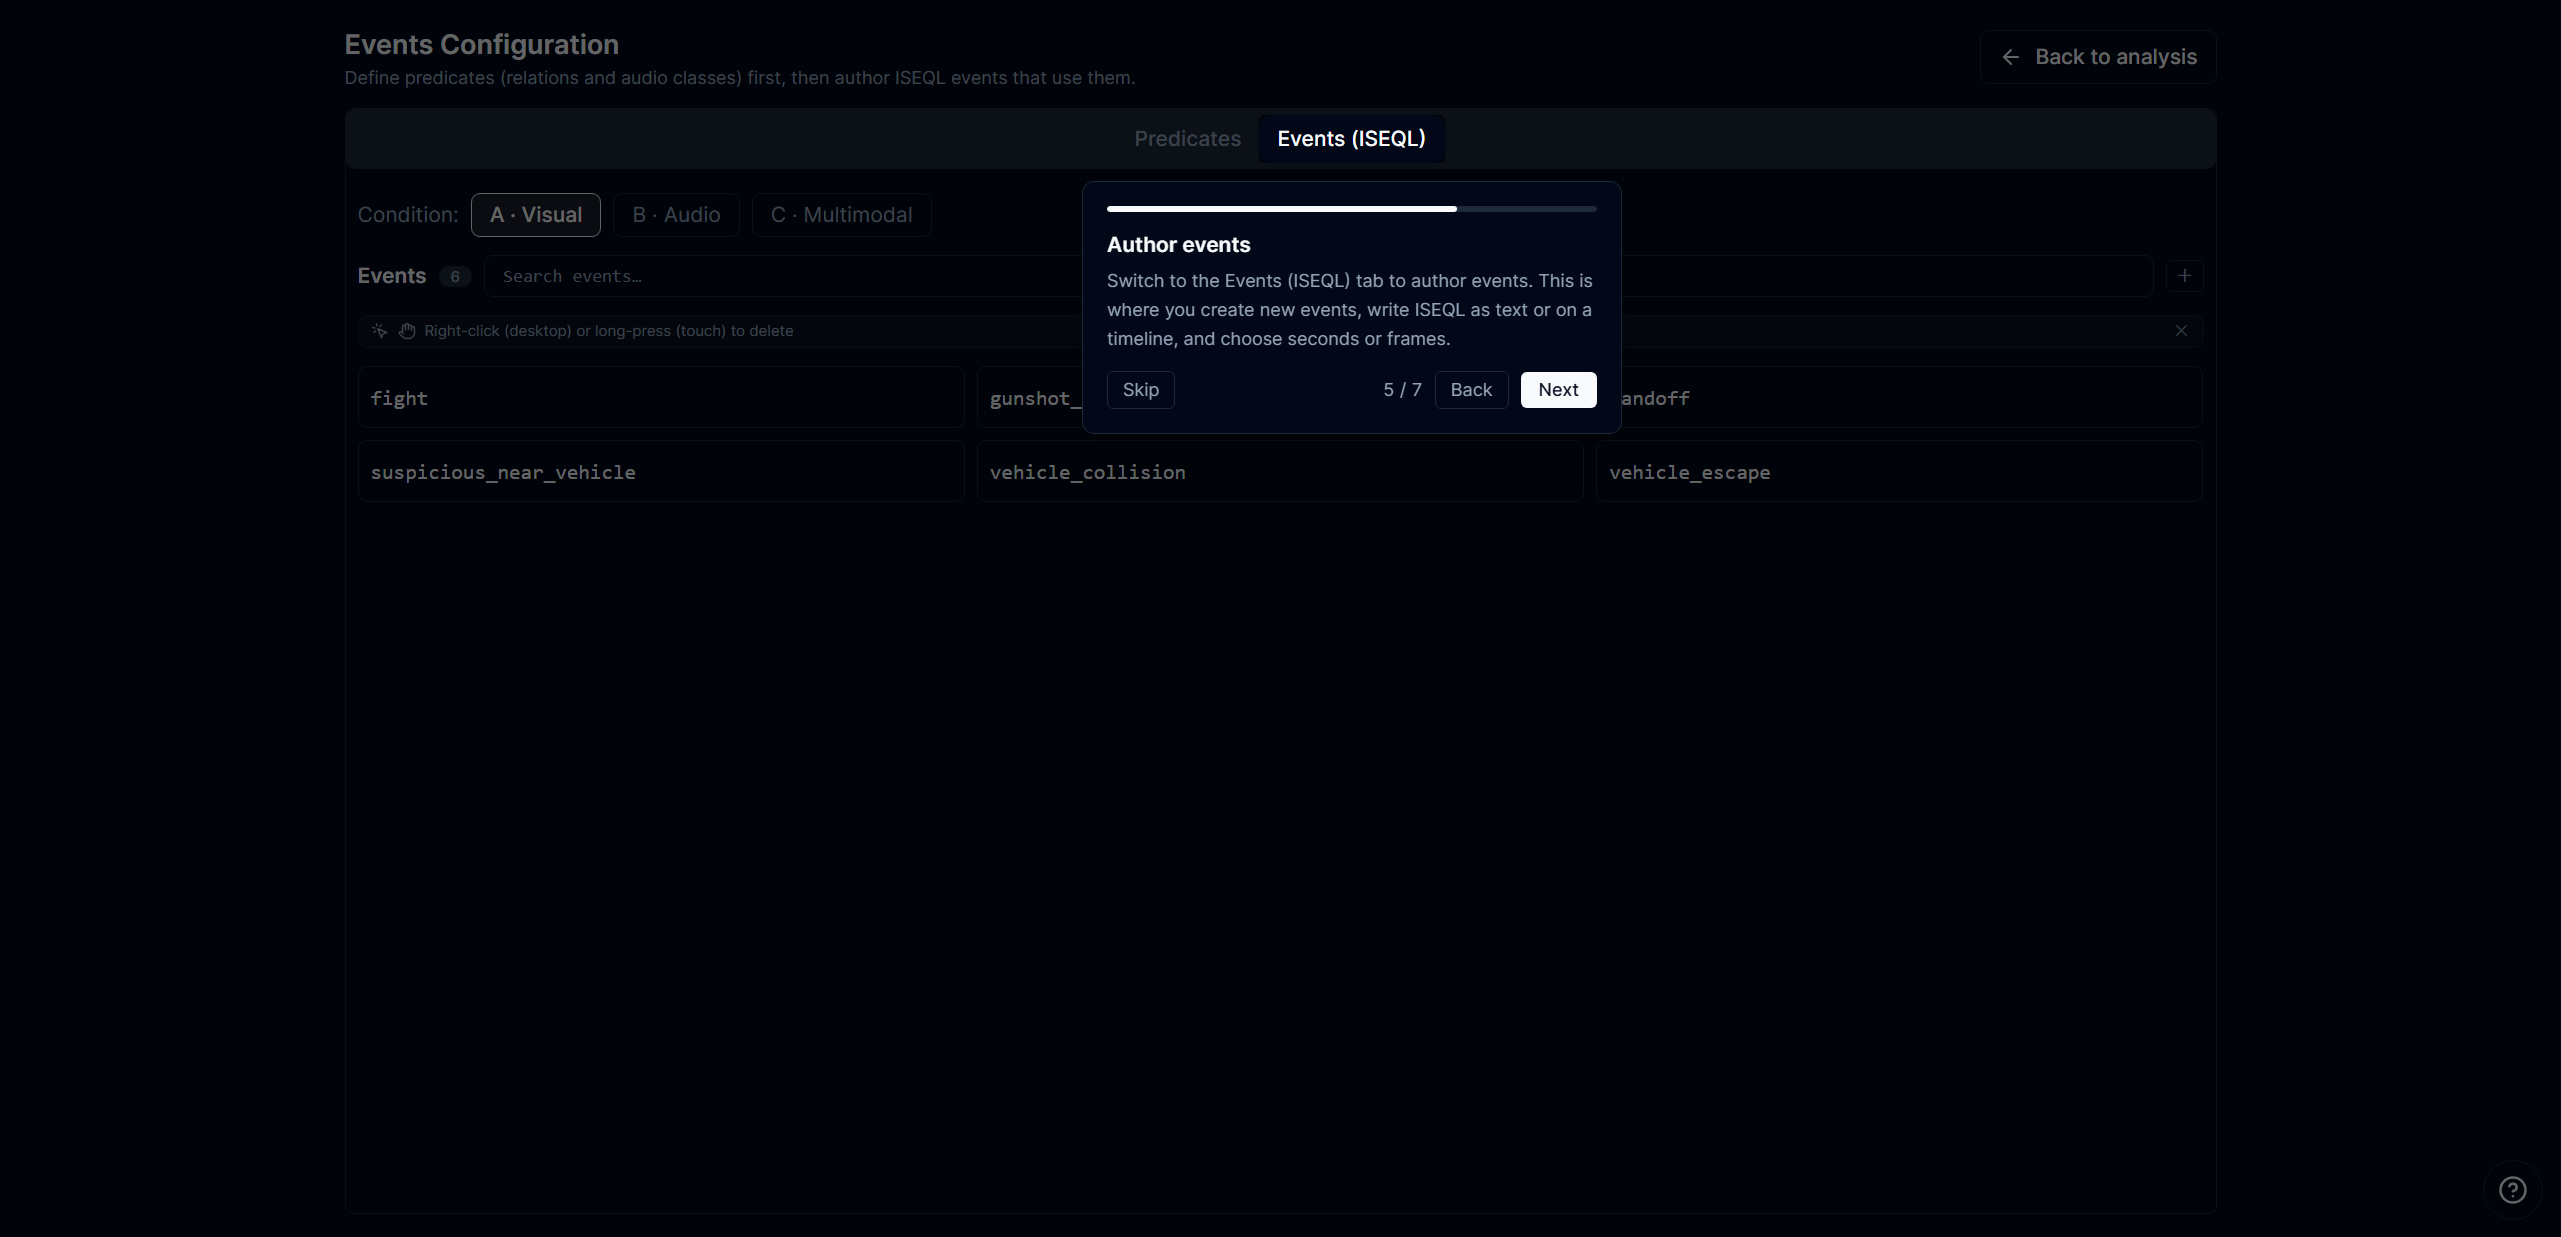
\includegraphics[width=0.92\textwidth]{Figures/appendix/cfg05_events_tab.png}
  \caption{Author events: switch to the Events (ISEQL) tab to author events.}
\end{figure}

\begin{figure}[H]
  \centering
  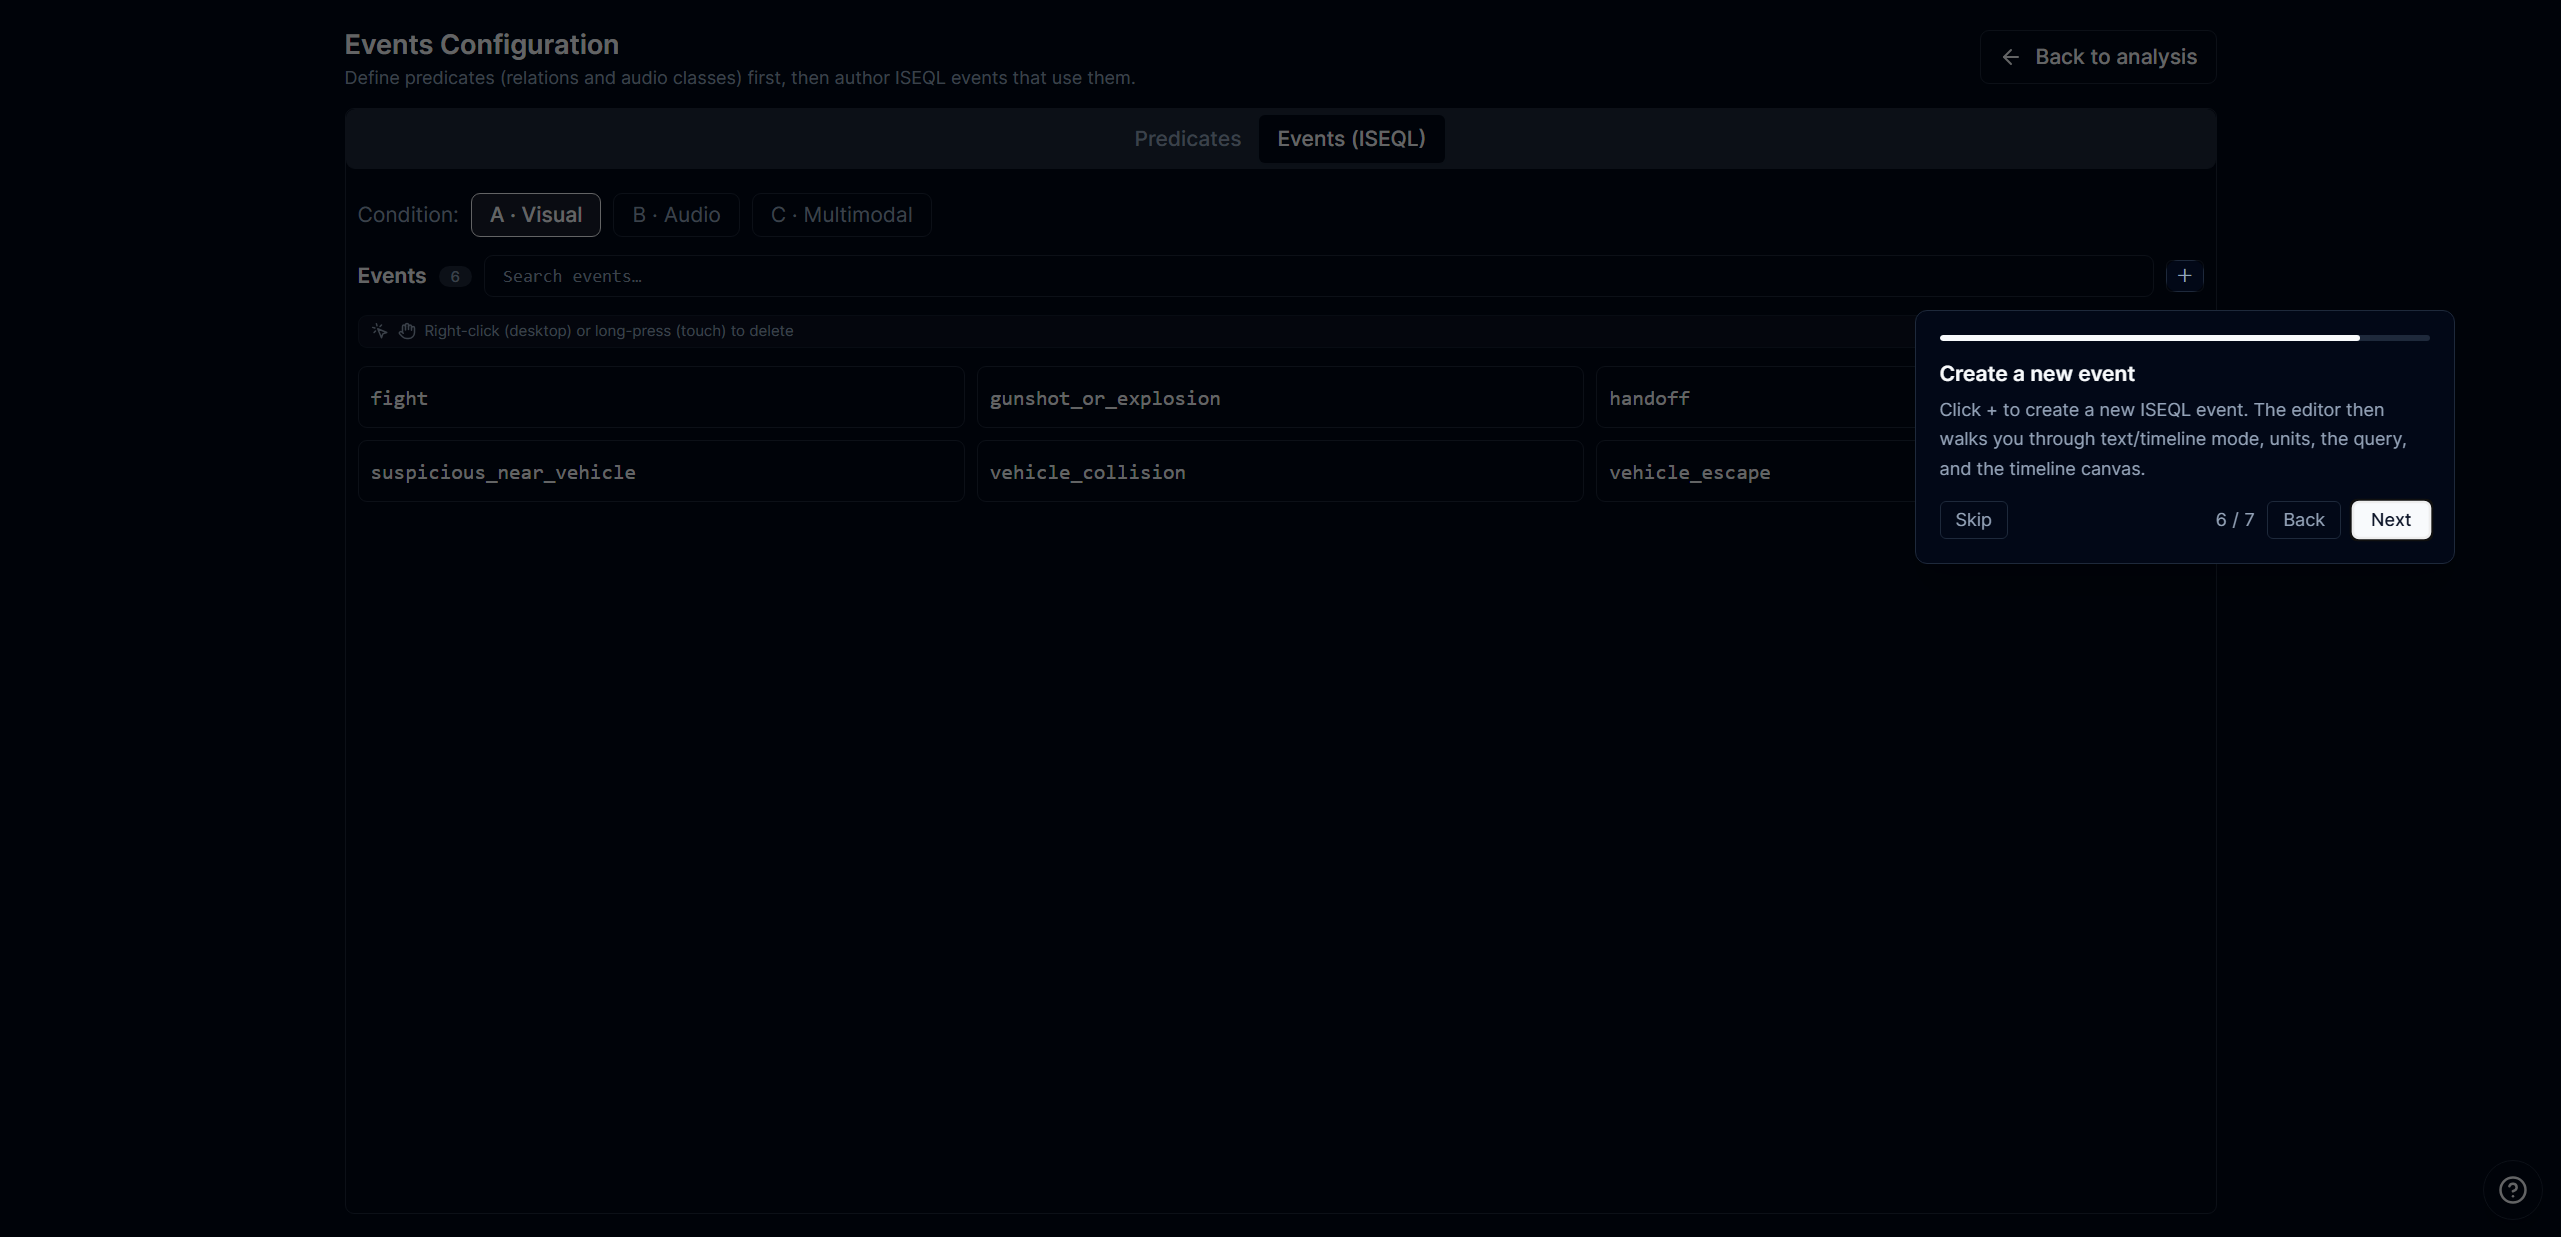
\includegraphics[width=0.92\textwidth]{Figures/appendix/cfg06_events_list.png}
  \caption{Event list: existing events appear here, click to edit.}
\end{figure}

\begin{figure}[H]
  \centering
  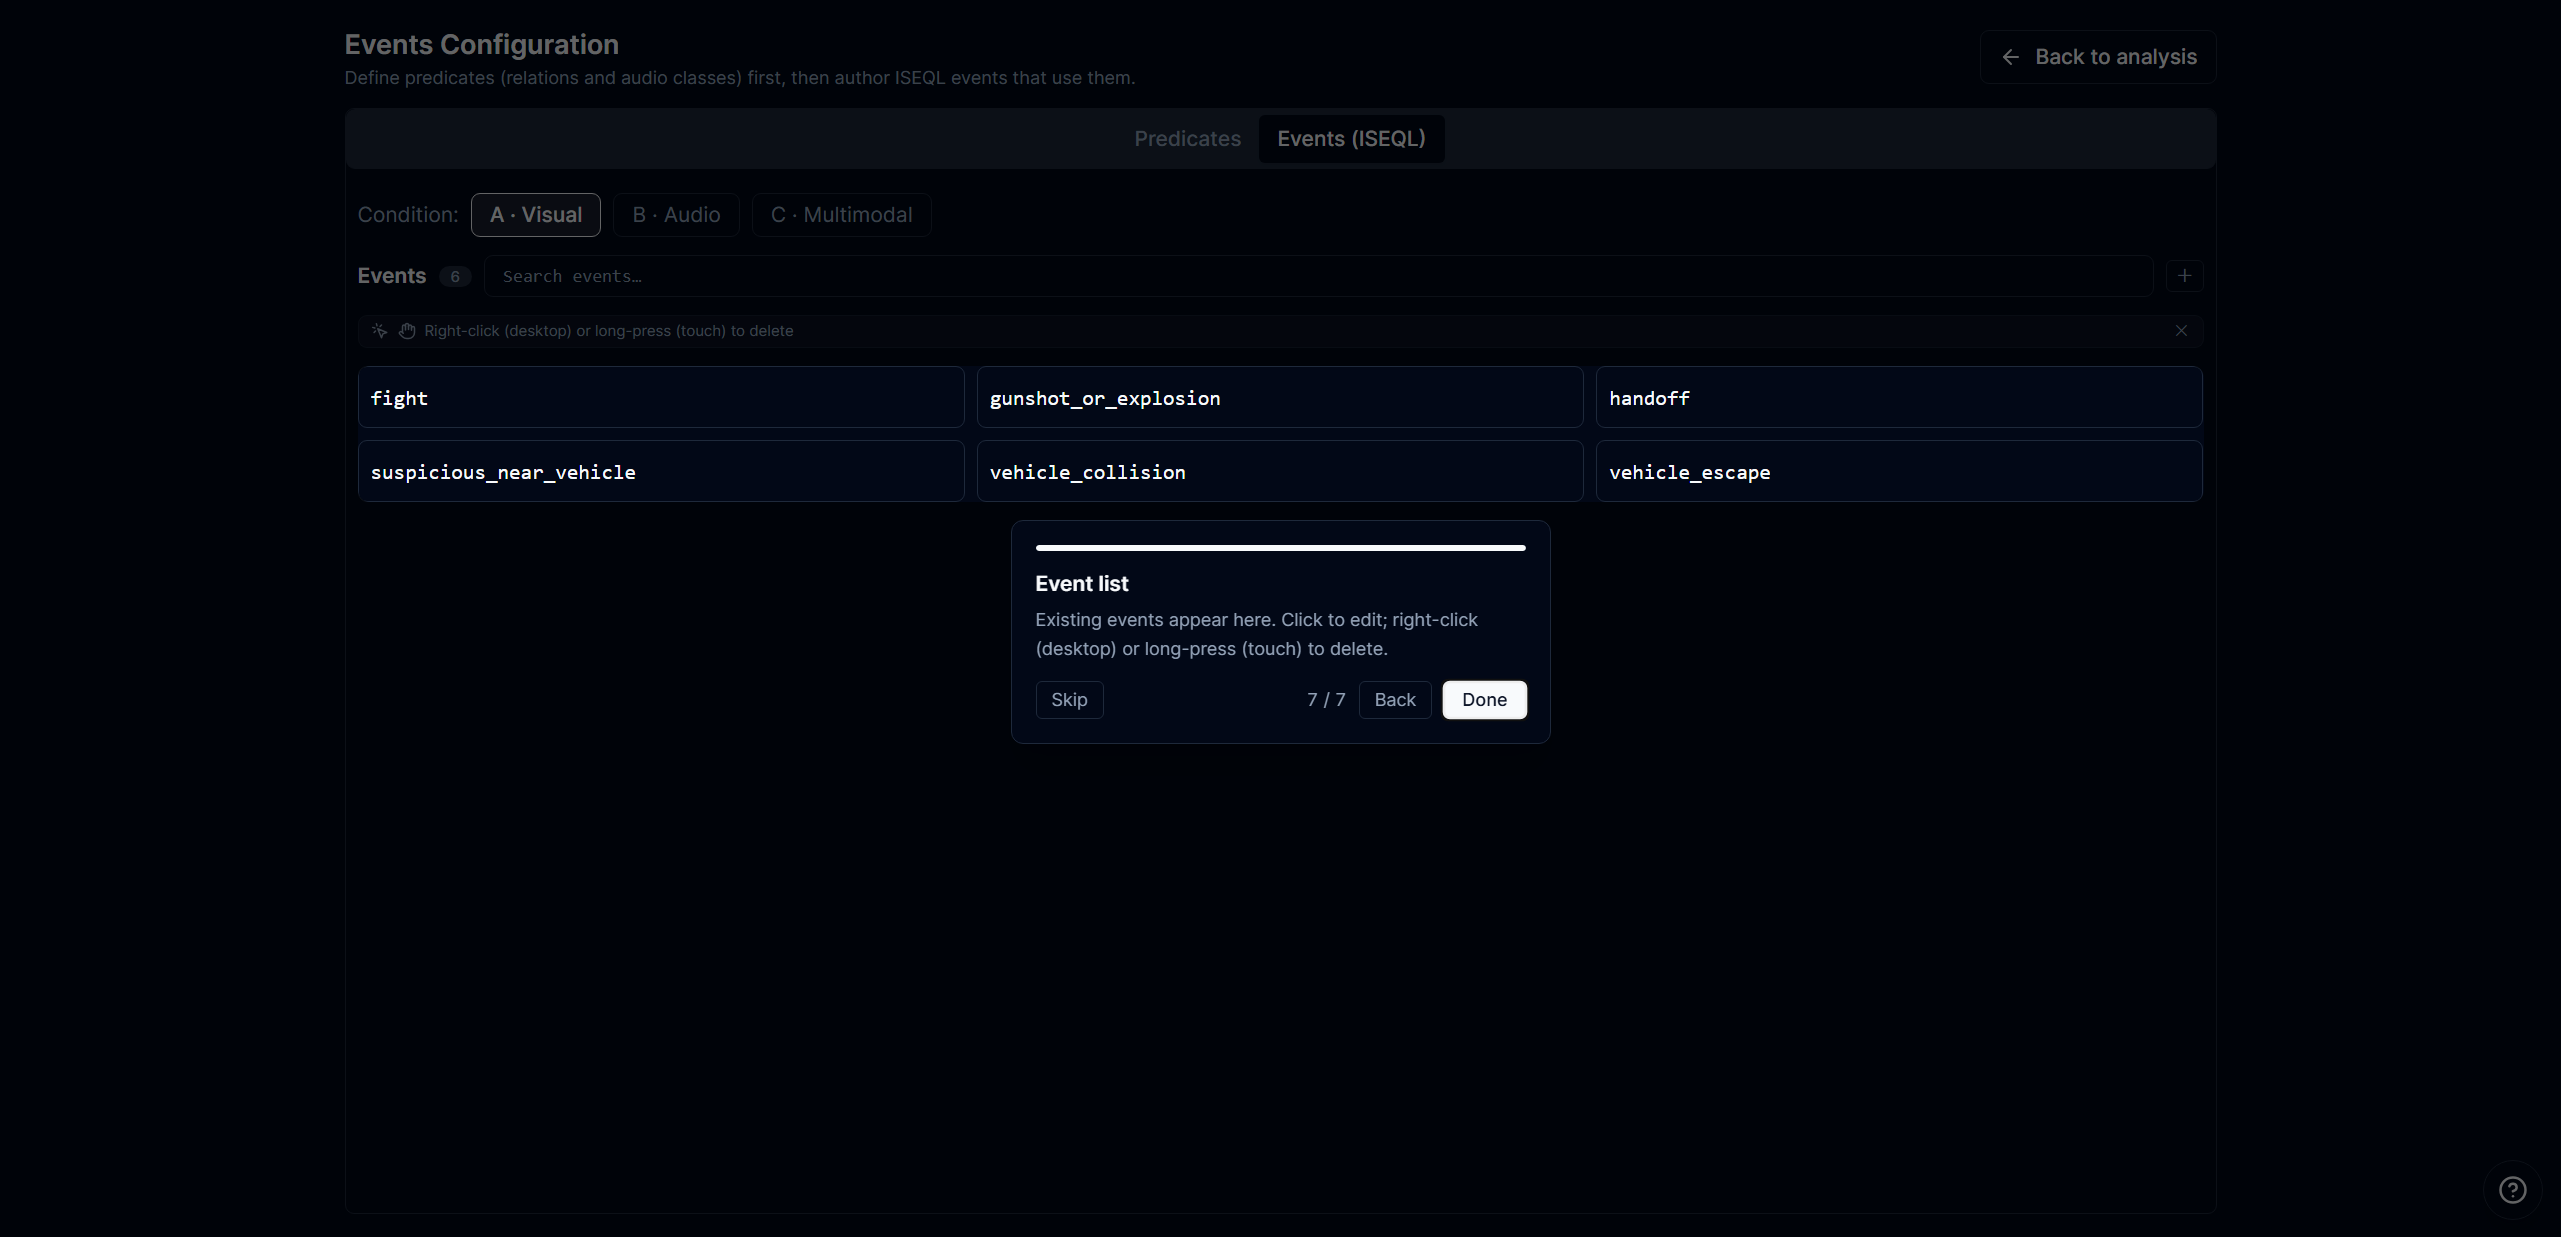
\includegraphics[width=0.92\textwidth]{Figures/appendix/cfg07_event_list_popup.png}
  \caption{Event list: right-click (desktop) or long-press (touch) to delete.}
\end{figure}

\begin{figure}[H]
  \centering
  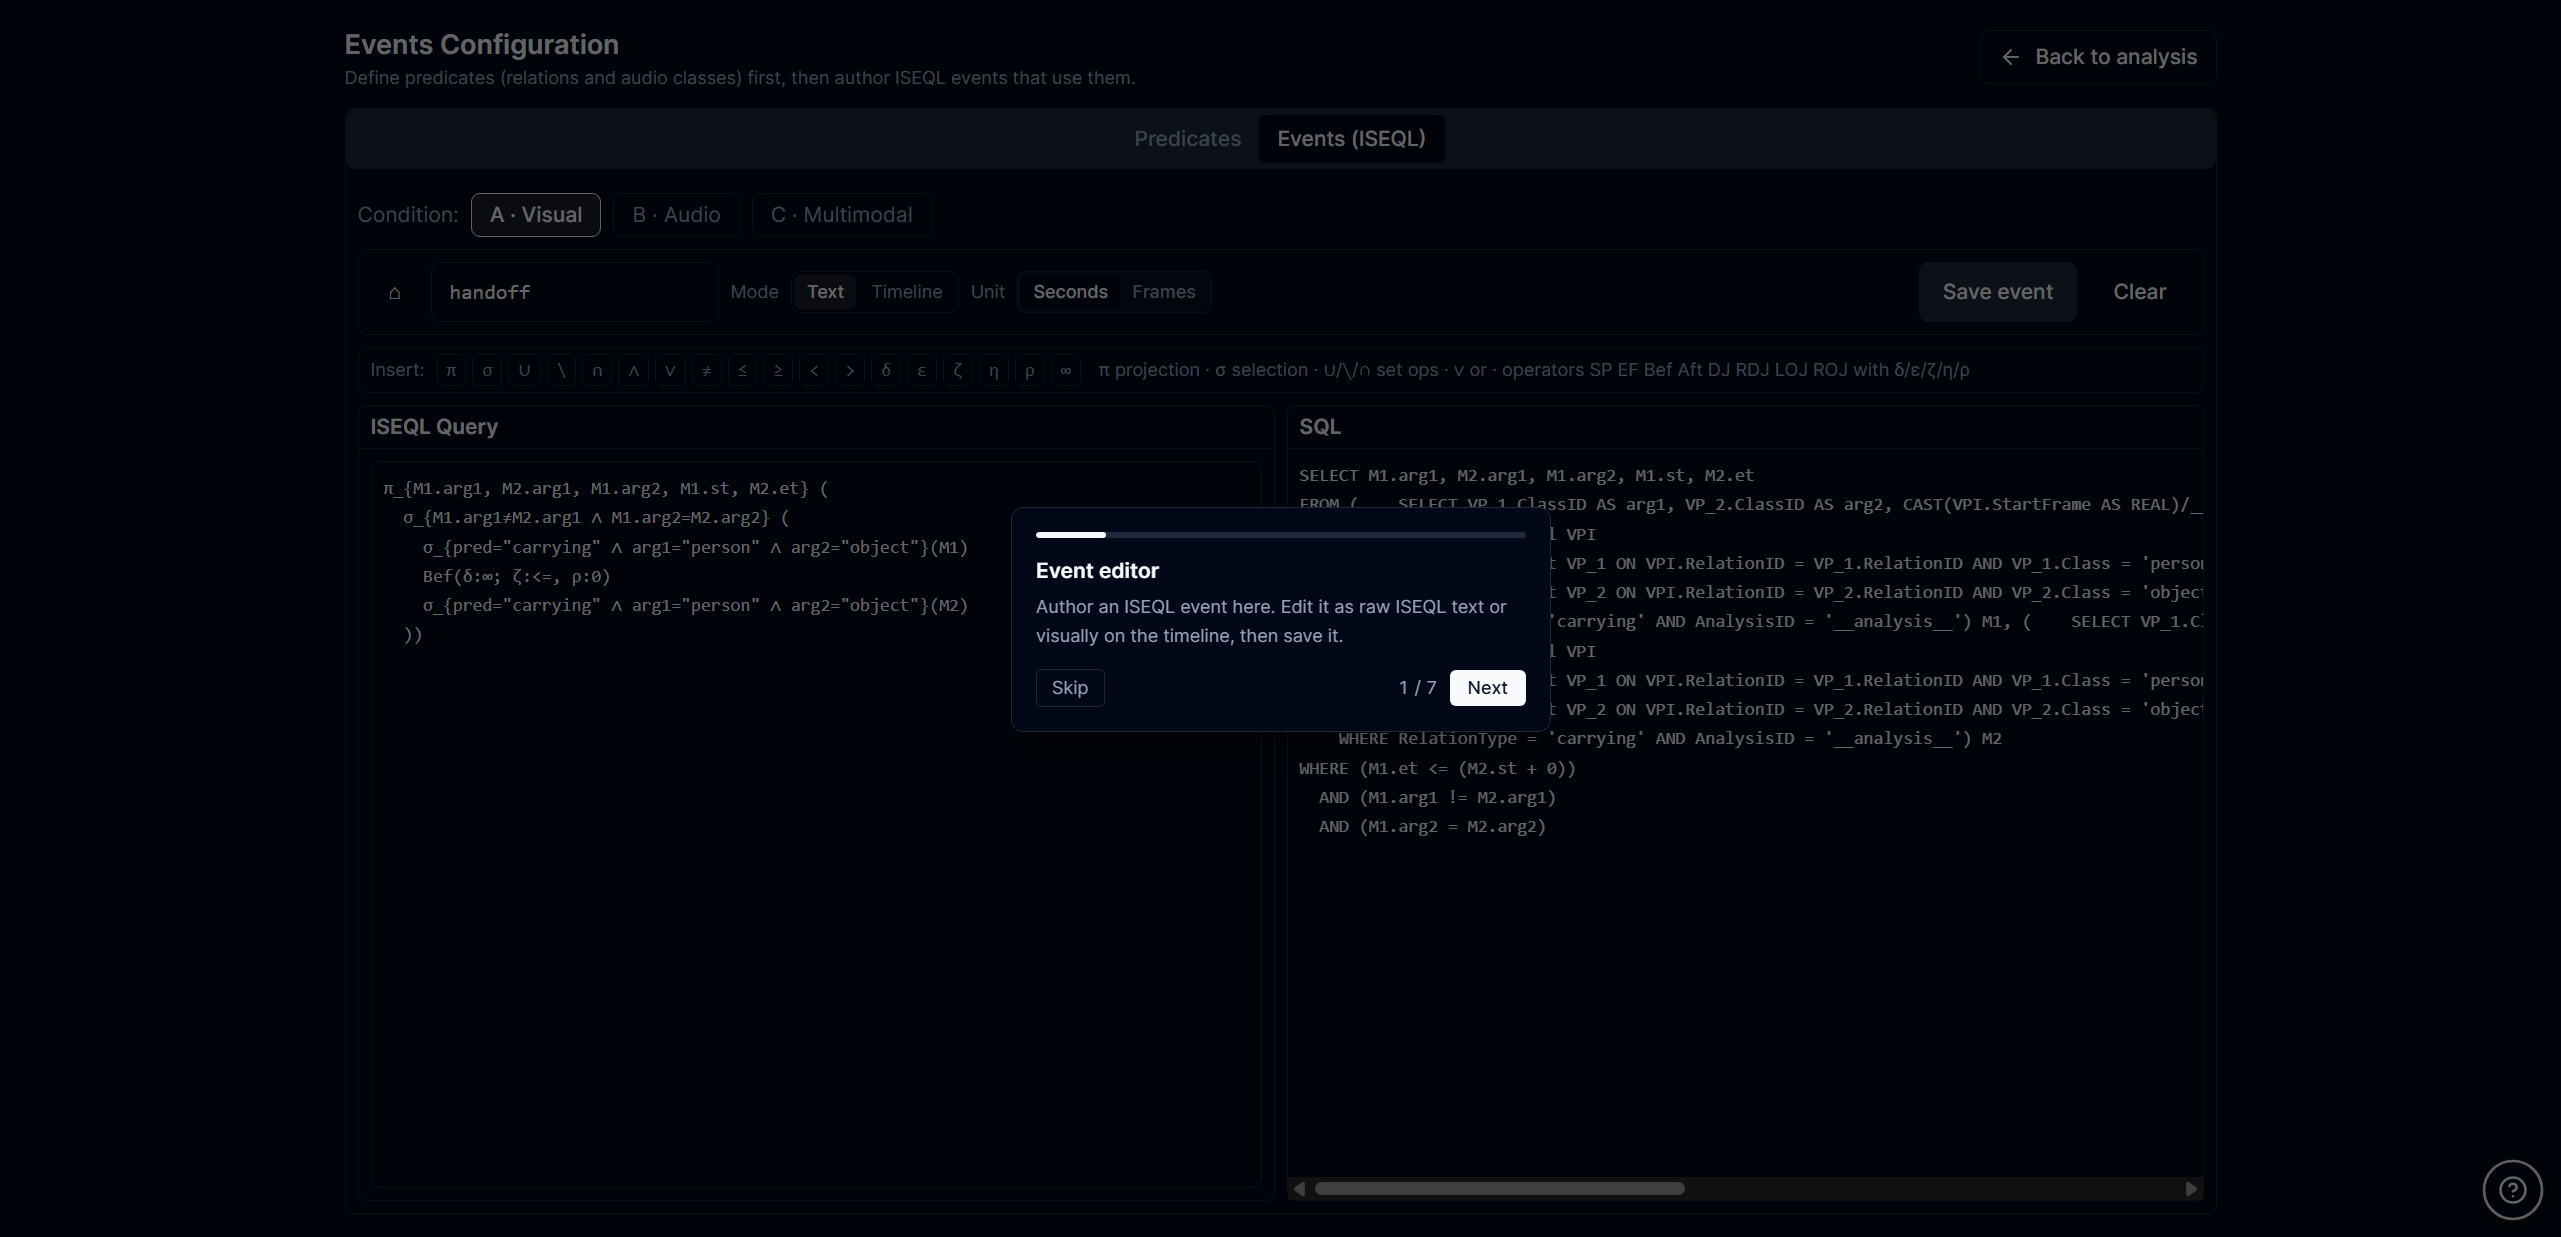
\includegraphics[width=0.92\textwidth]{Figures/appendix/cfg08_editor.png}
  \caption{Event editor: author an ISEQL event as raw text or visually on the timeline.}
\end{figure}

\begin{figure}[H]
  \centering
  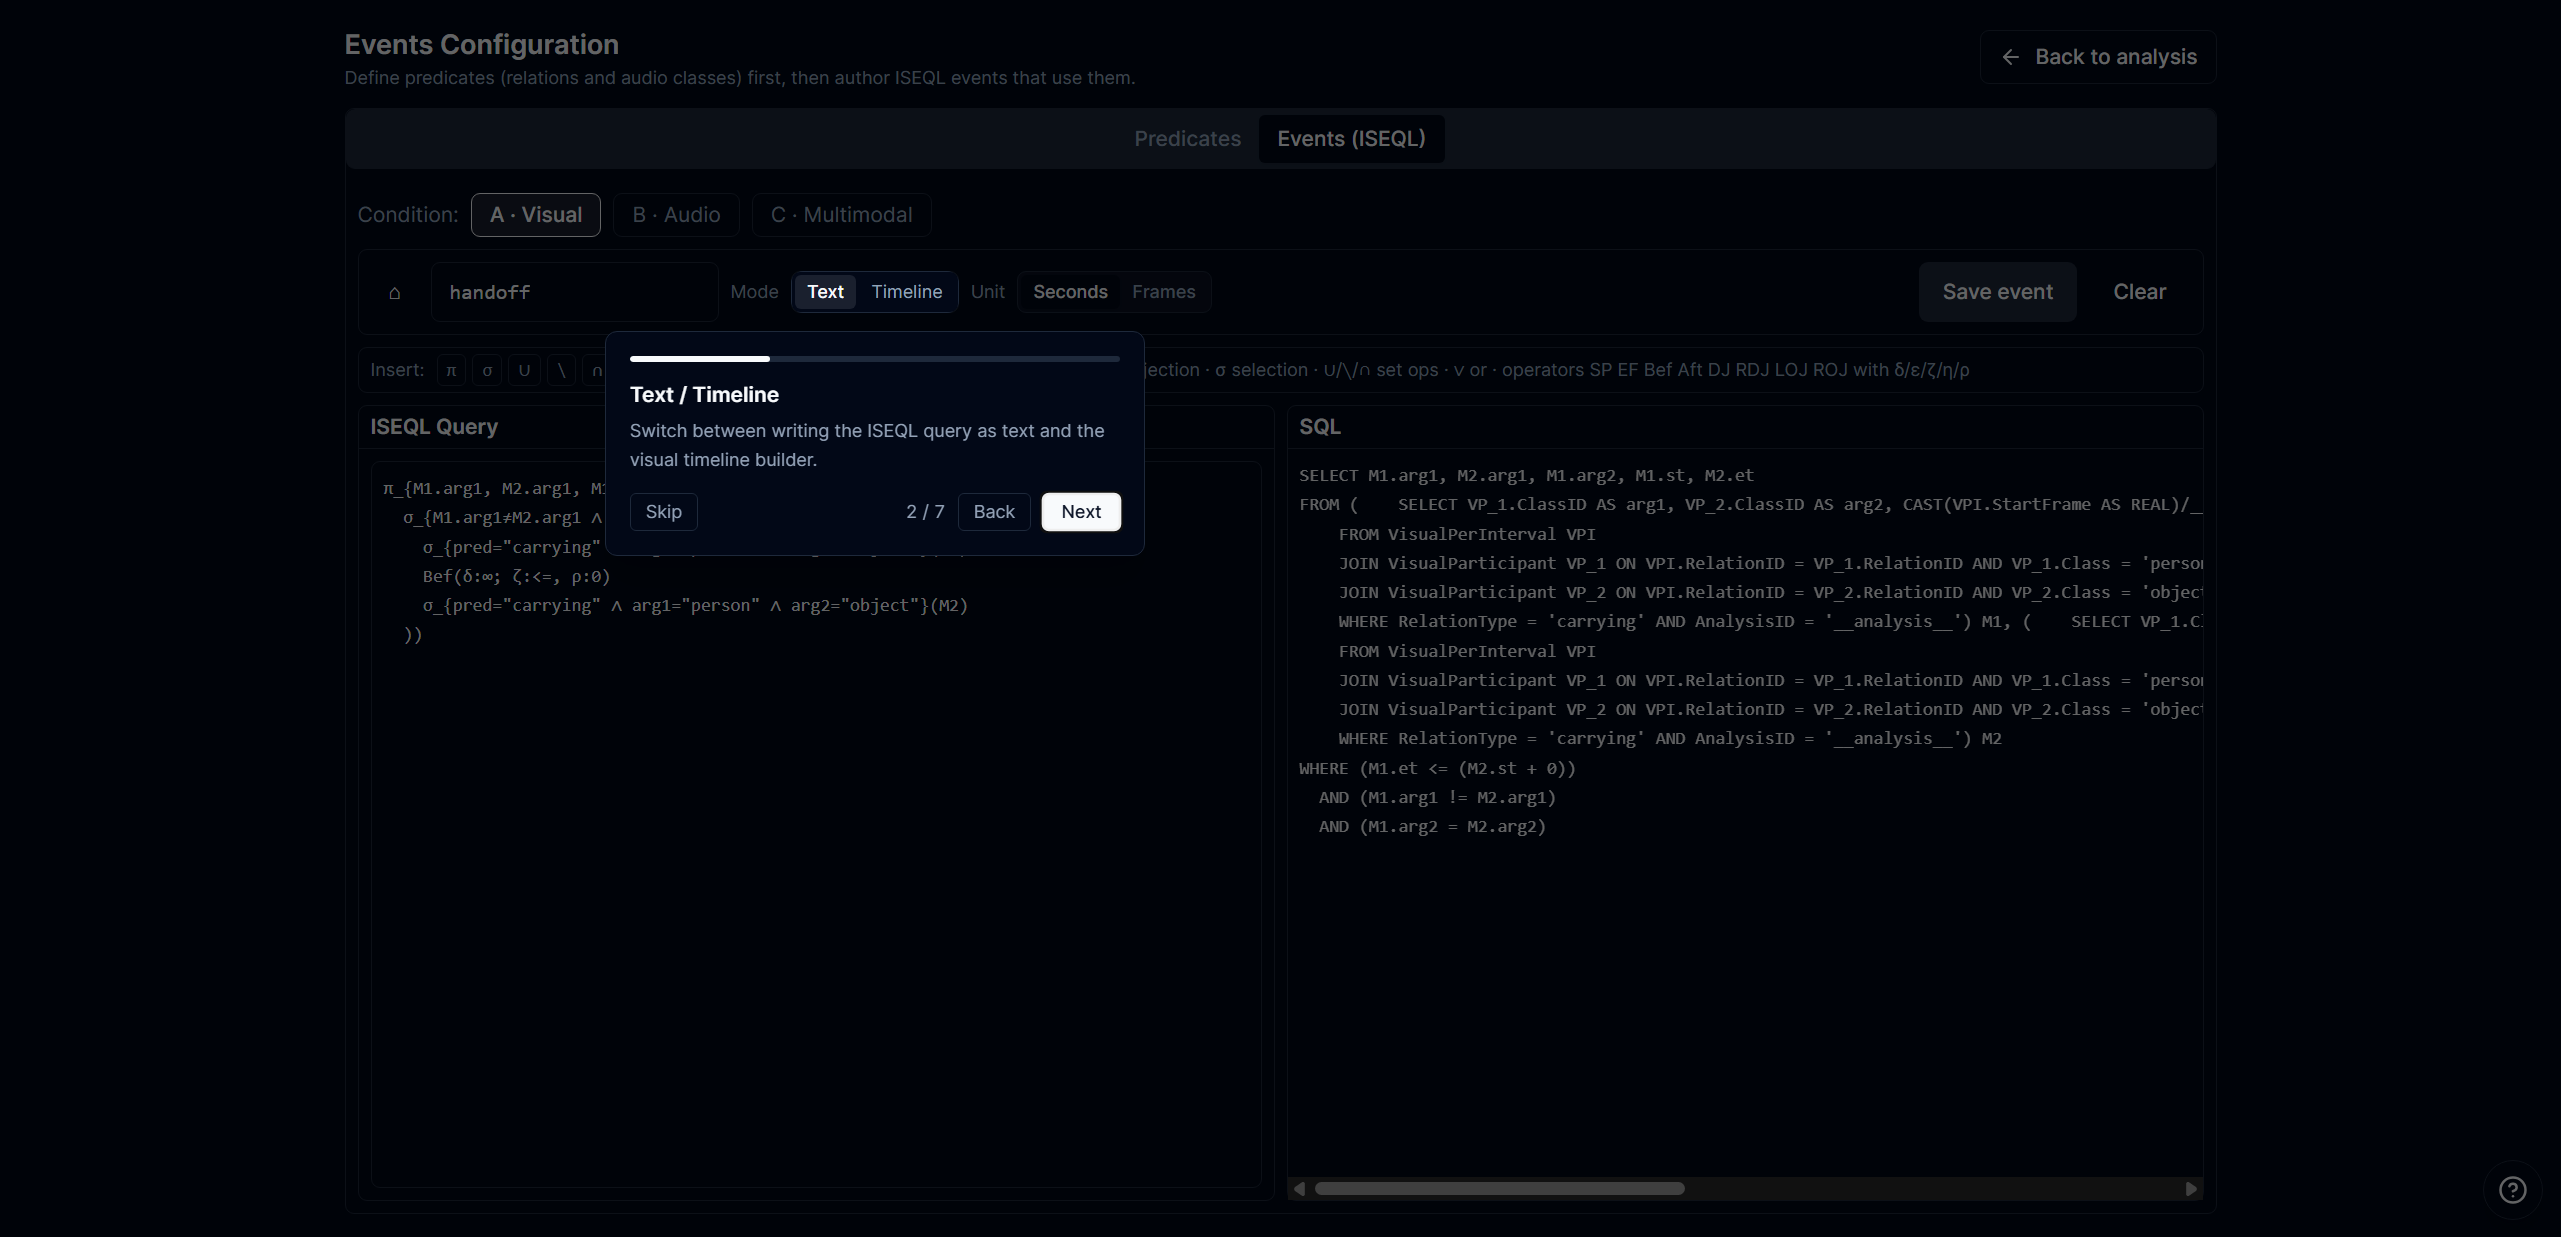
\includegraphics[width=0.92\textwidth]{Figures/appendix/cfg09_mode.png}
  \caption{Text / Timeline: switch between writing the ISEQL query as text and using the visual timeline builder.}
\end{figure}

\begin{figure}[H]
  \centering
  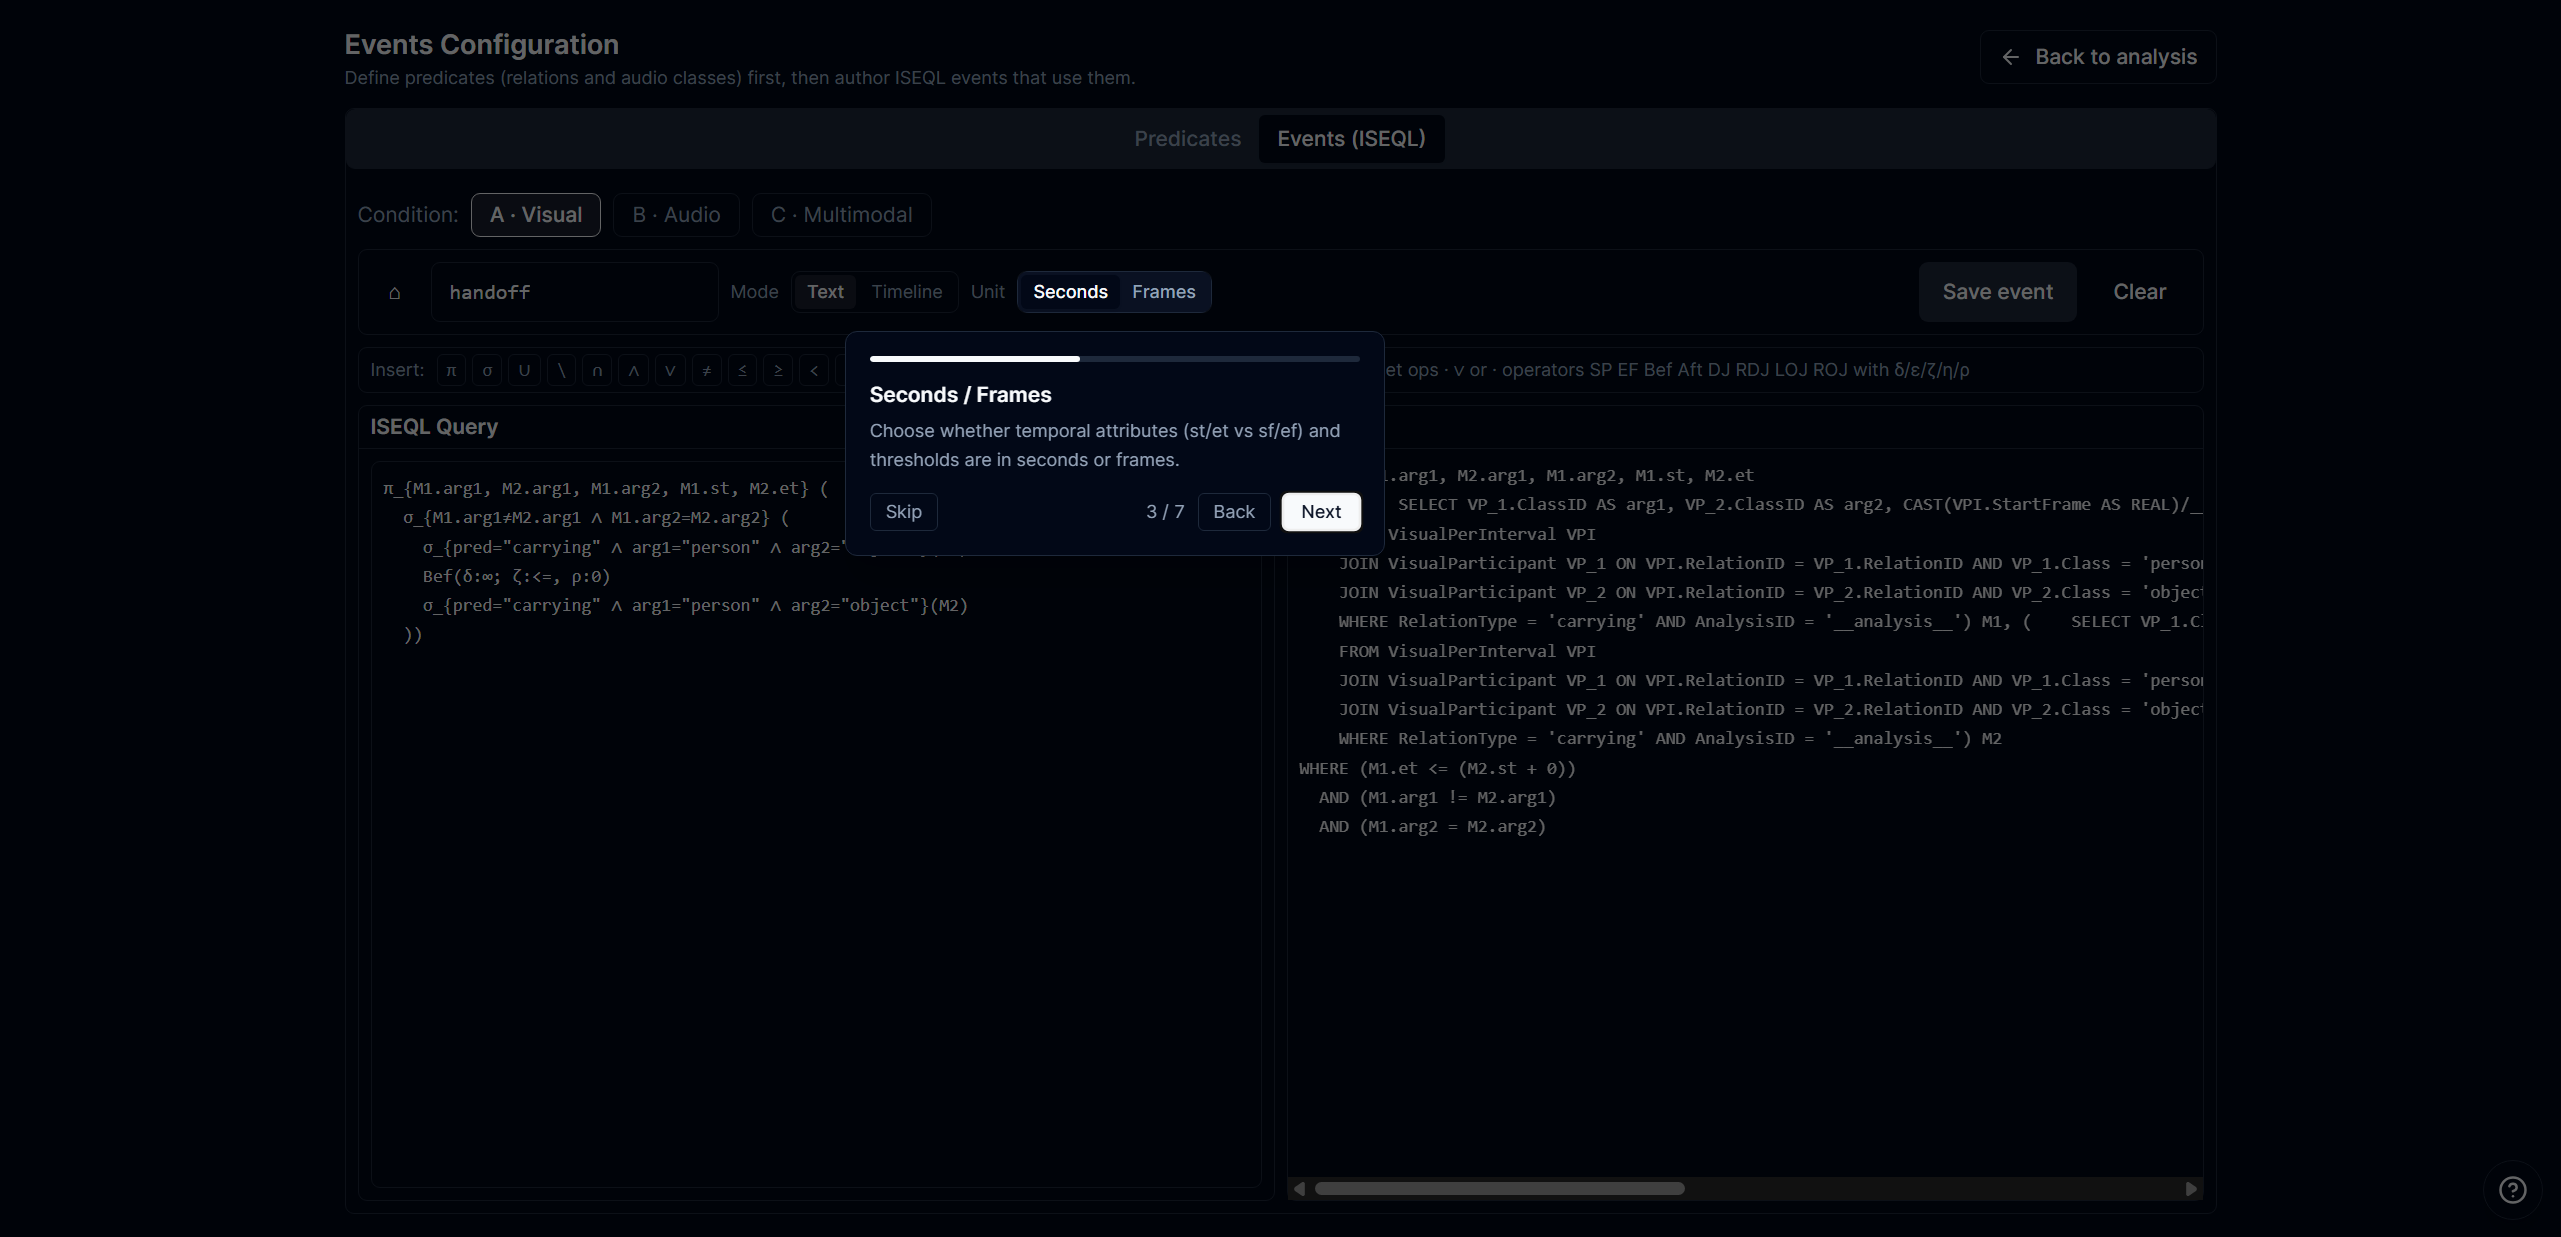
\includegraphics[width=0.92\textwidth]{Figures/appendix/cfg10_units.png}
  \caption{Seconds / Frames: choose whether temporal attributes (st/et vs sf/ef) are in seconds or frames.}
\end{figure}

\begin{figure}[H]
  \centering
  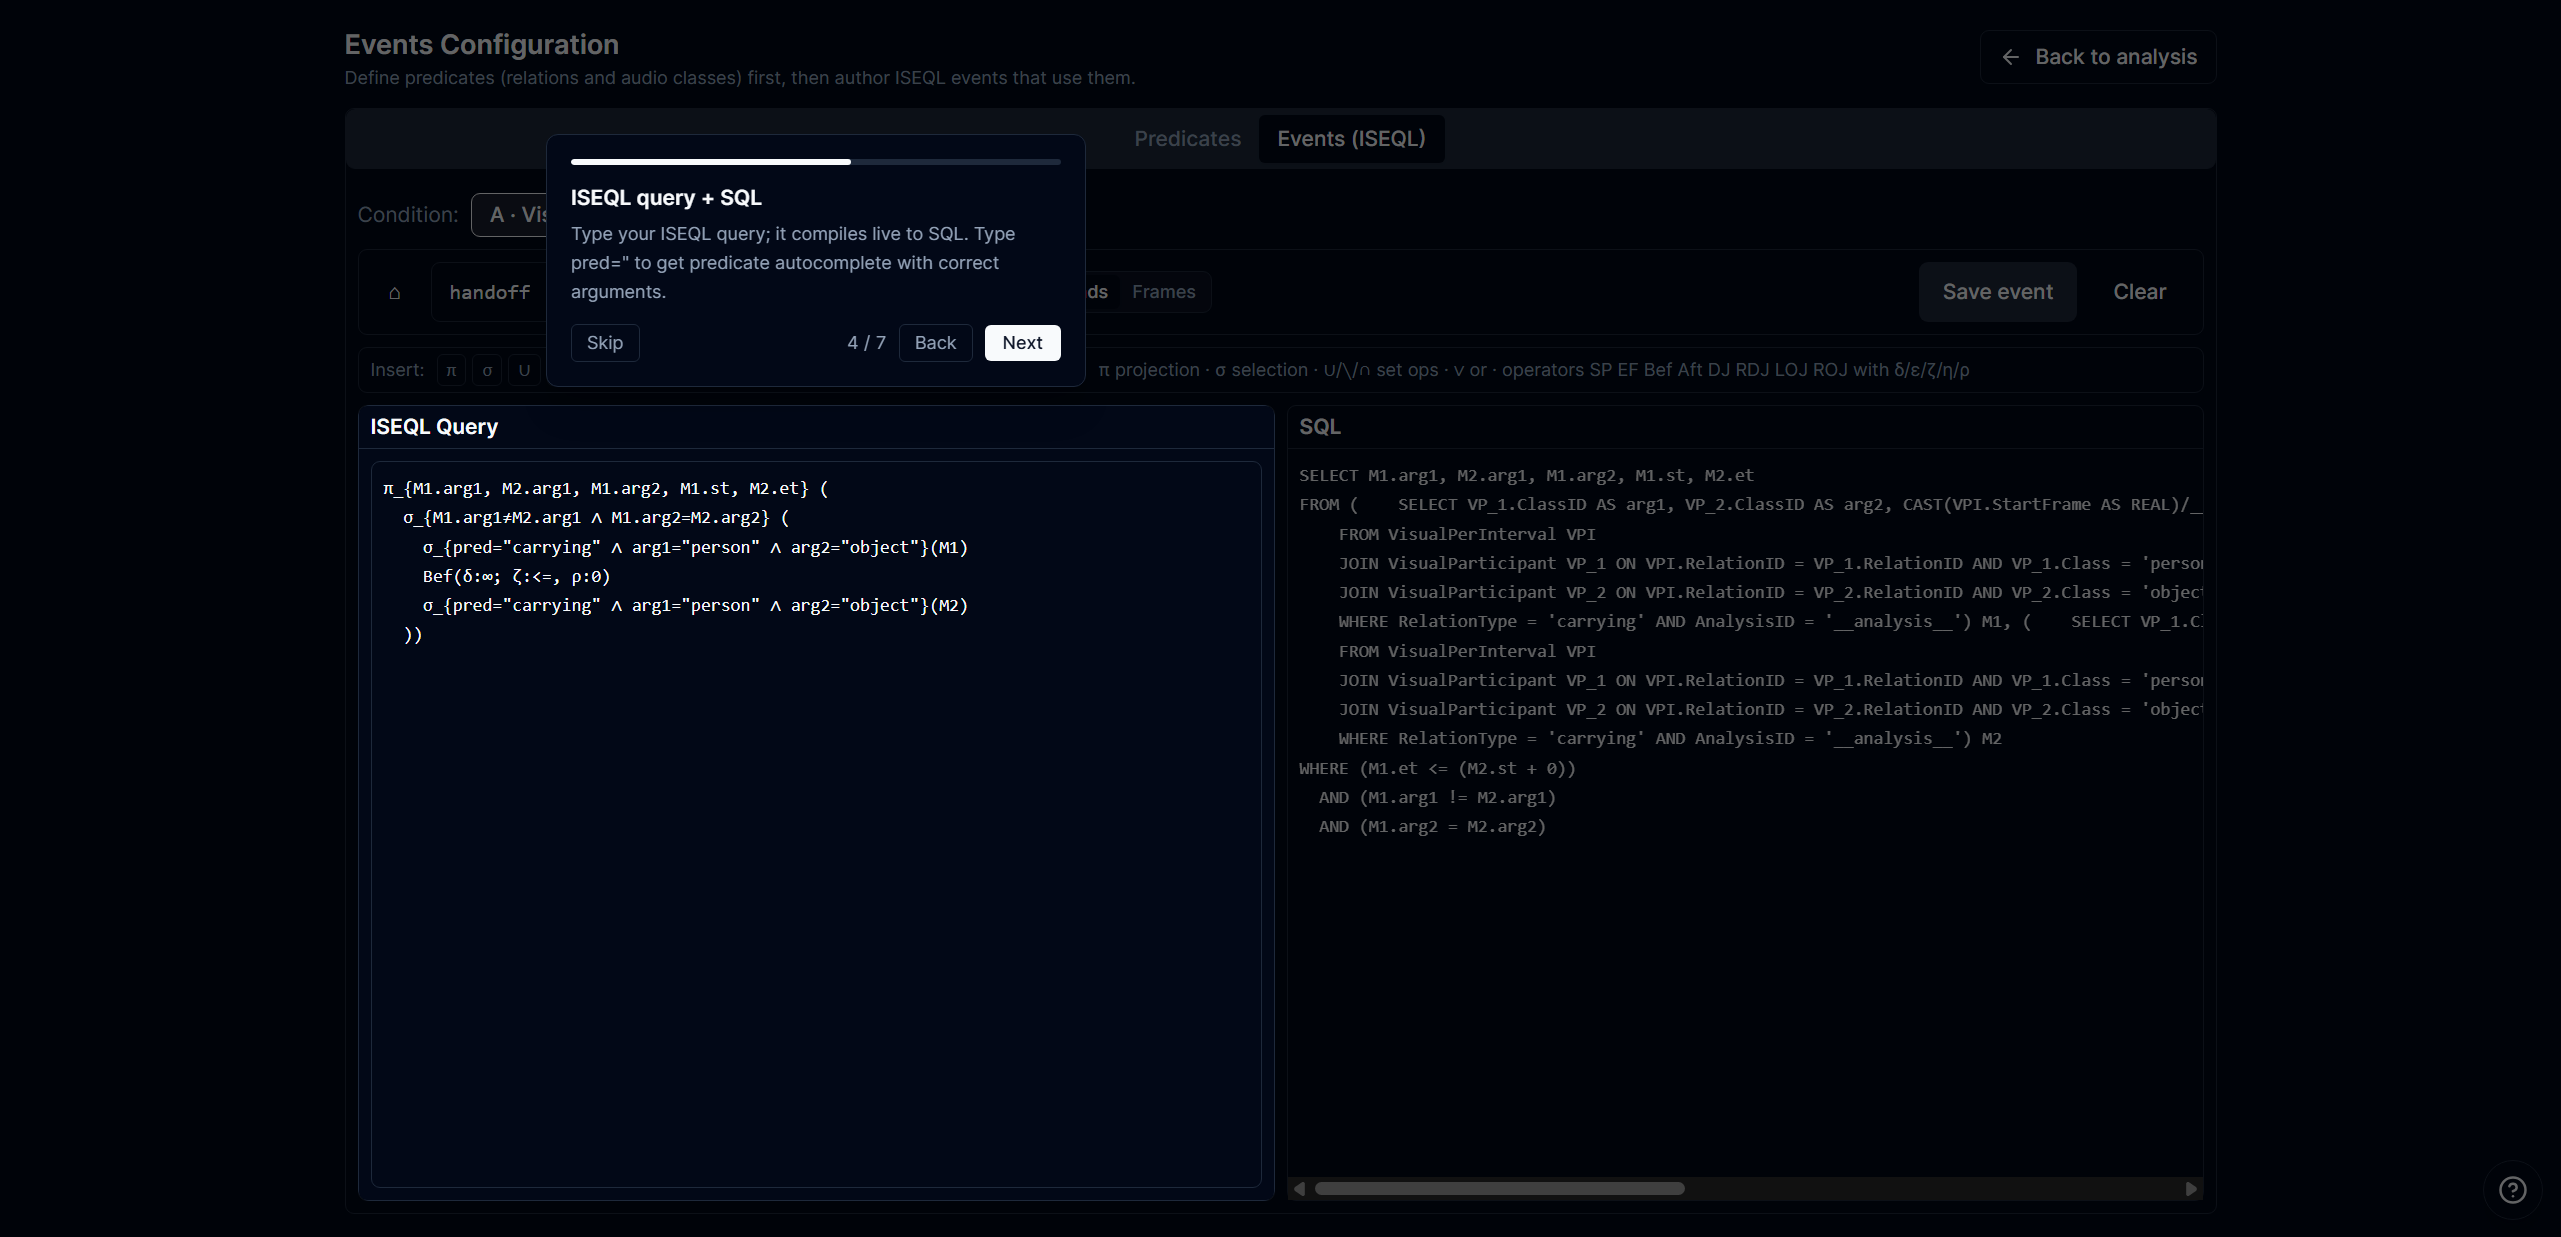
\includegraphics[width=0.92\textwidth]{Figures/appendix/cfg11_query_sql.png}
  \caption{ISEQL query + SQL: type the ISEQL query; it compiles live to SQL.}
\end{figure}

\begin{figure}[H]
  \centering
  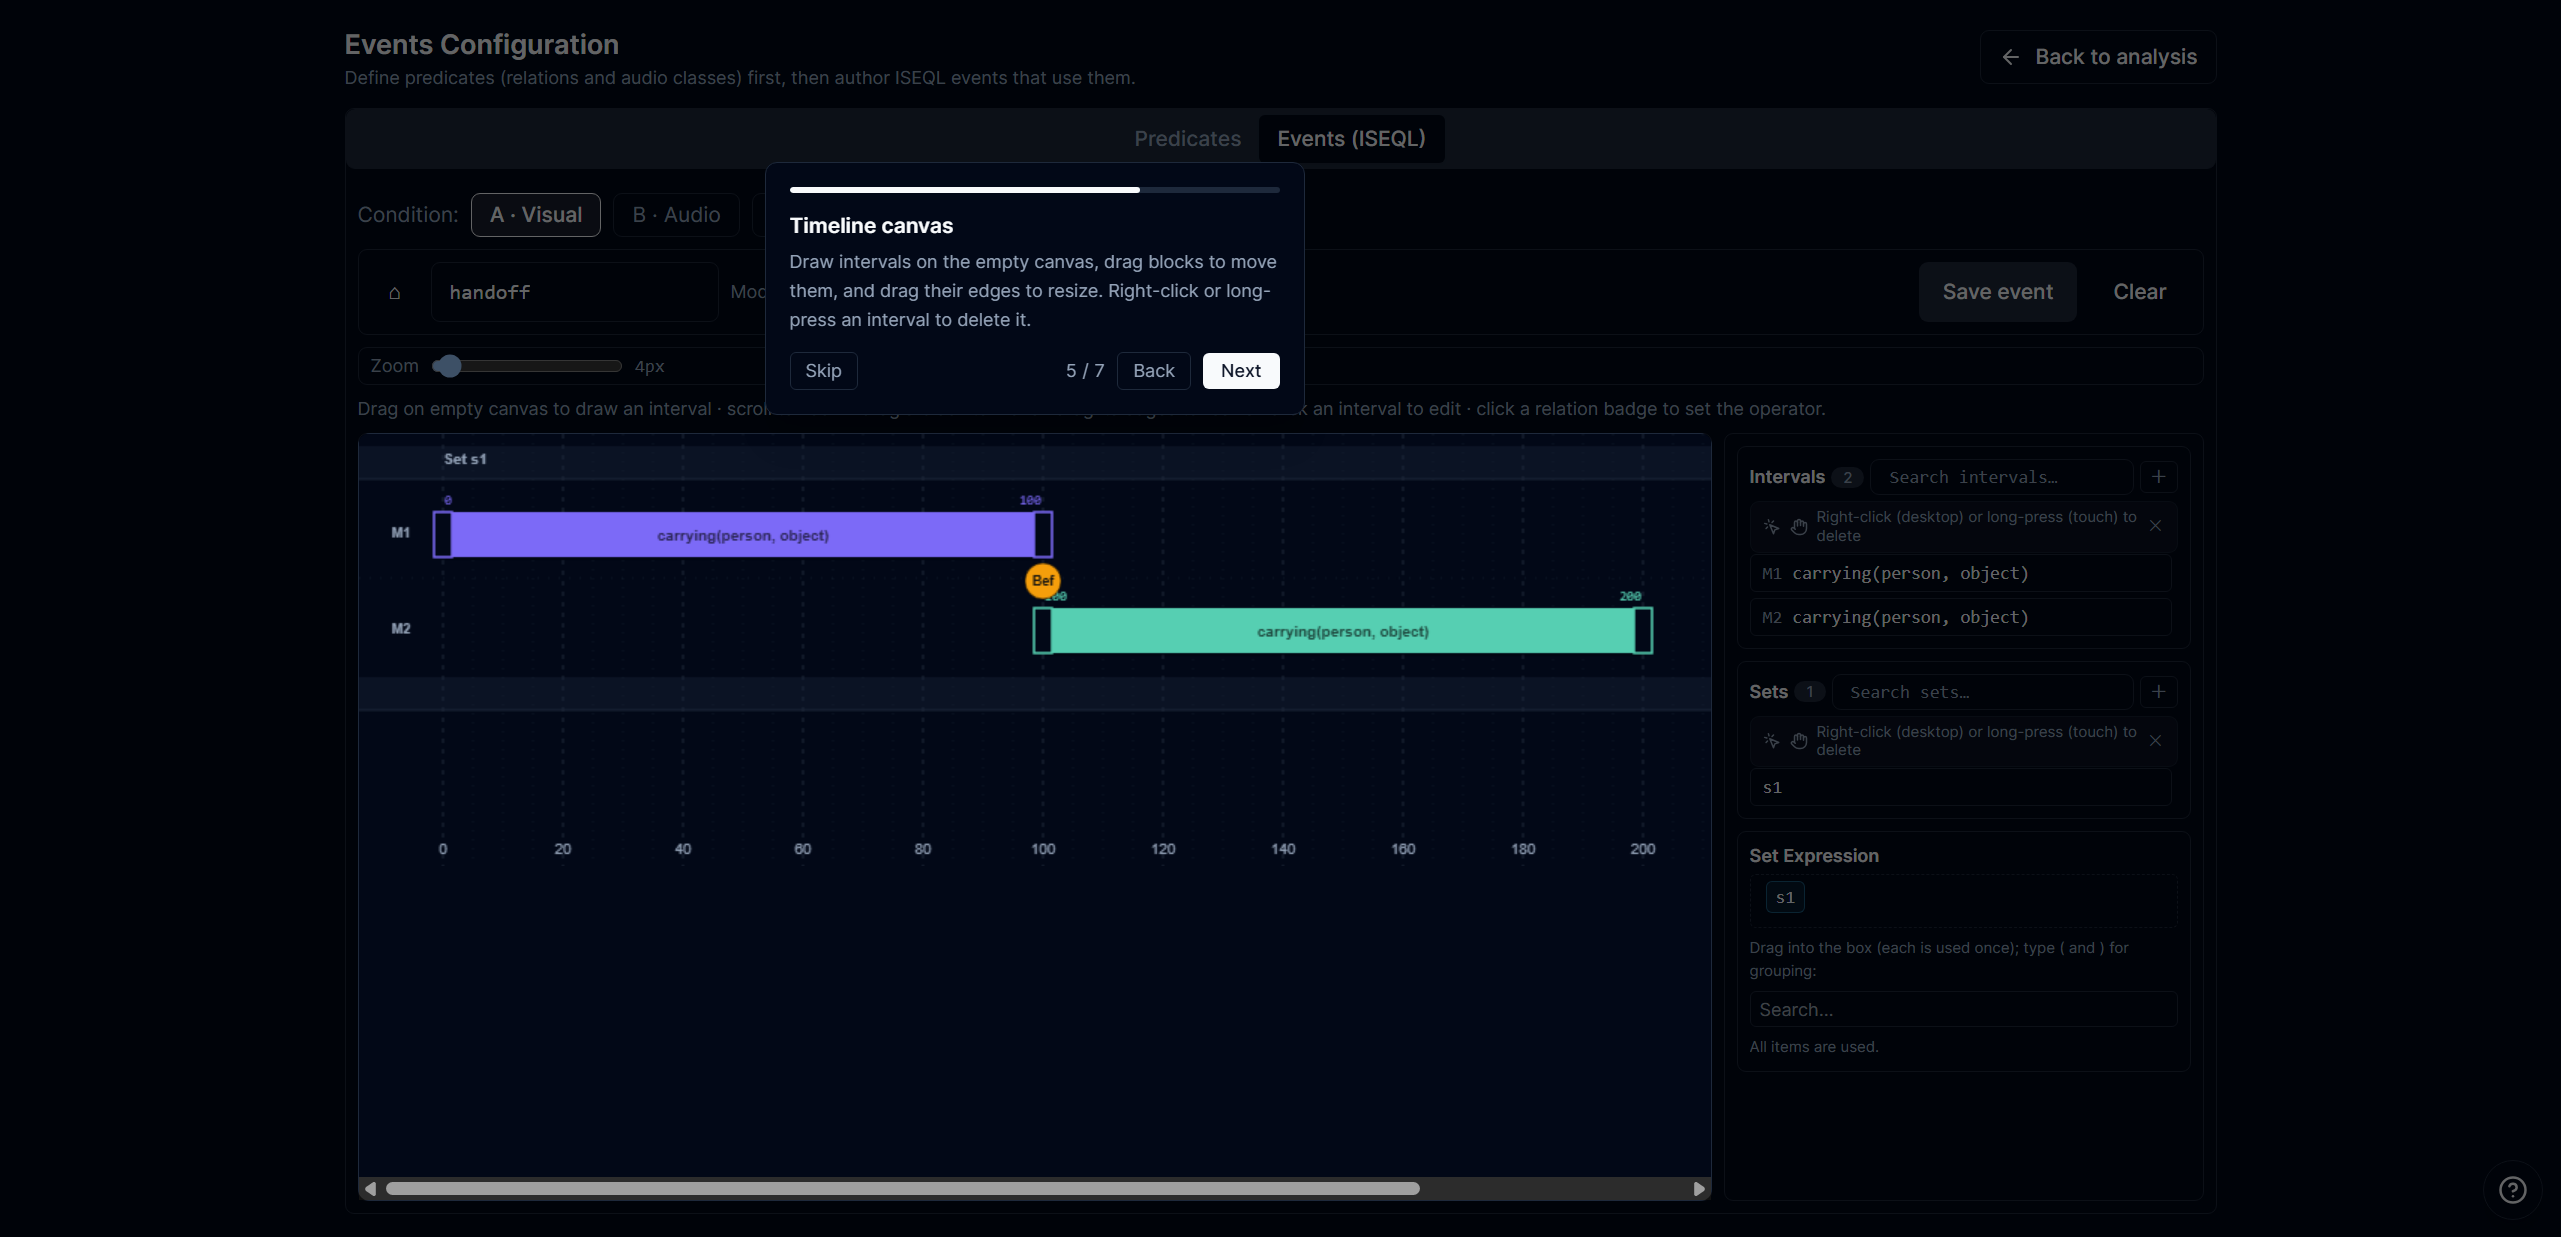
\includegraphics[width=0.92\textwidth]{Figures/appendix/cfg12_timeline.png}
  \caption{Timeline canvas: draw intervals, drag blocks to move them, and drag their edges to resize.}
\end{figure}

\begin{figure}[H]
  \centering
  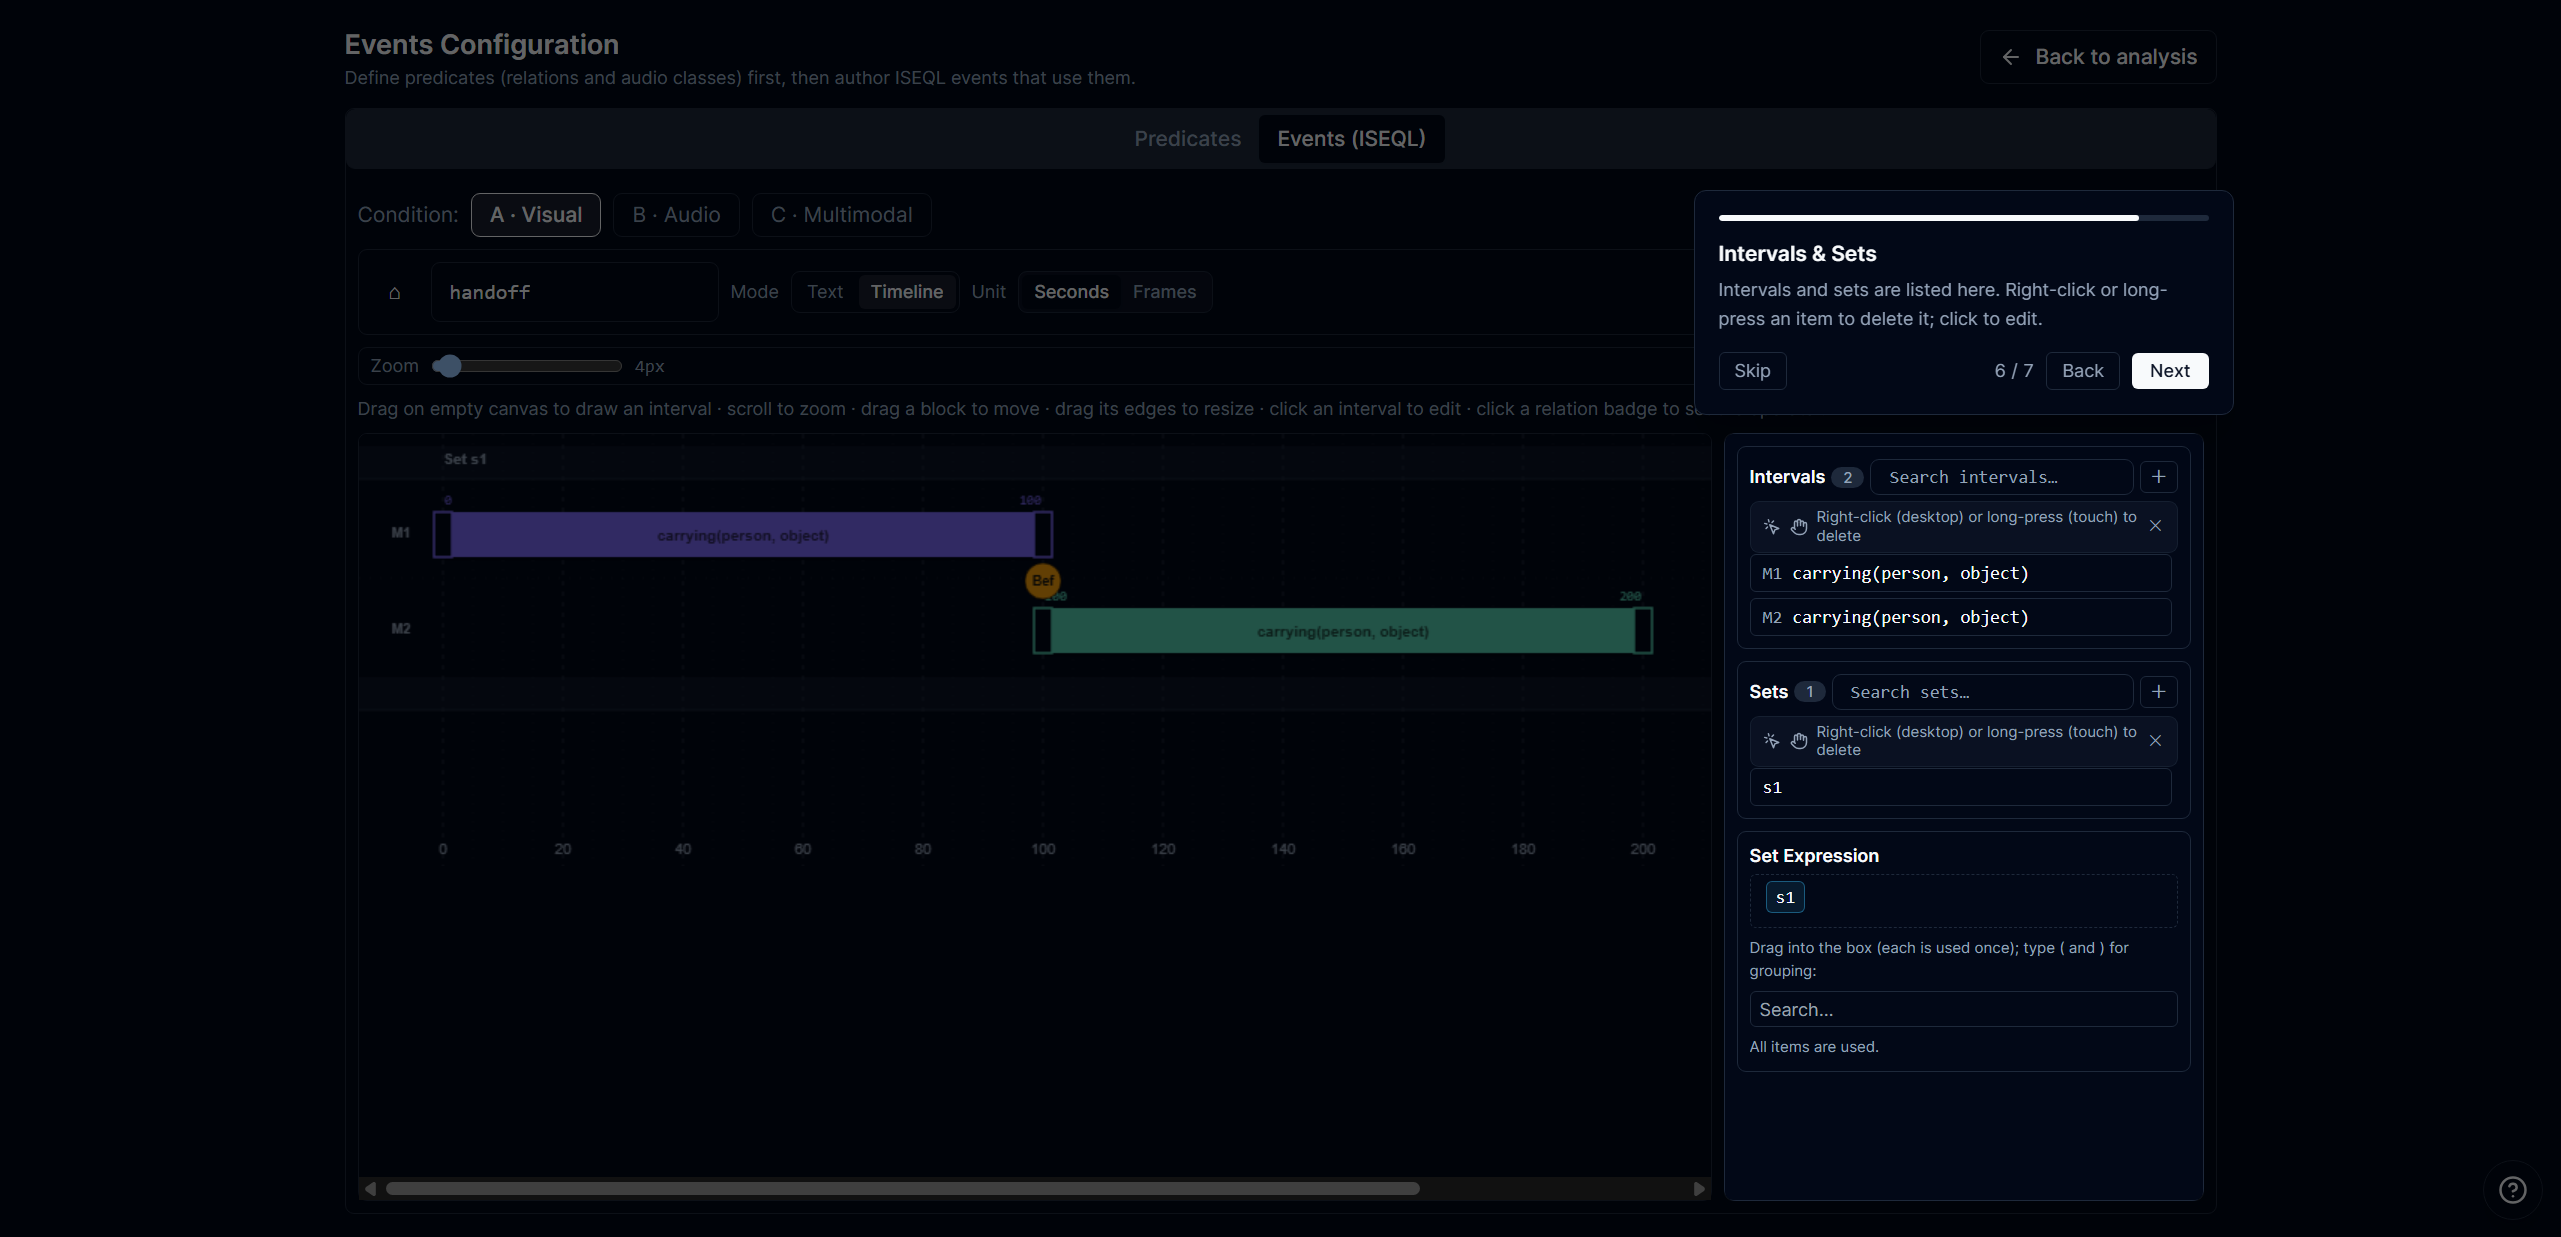
\includegraphics[width=0.92\textwidth]{Figures/appendix/cfg13_timeline_clean.png}
  \caption{Intervals and sets: intervals and sets are listed here; click an item to edit.}
\end{figure}

\begin{figure}[H]
  \centering
  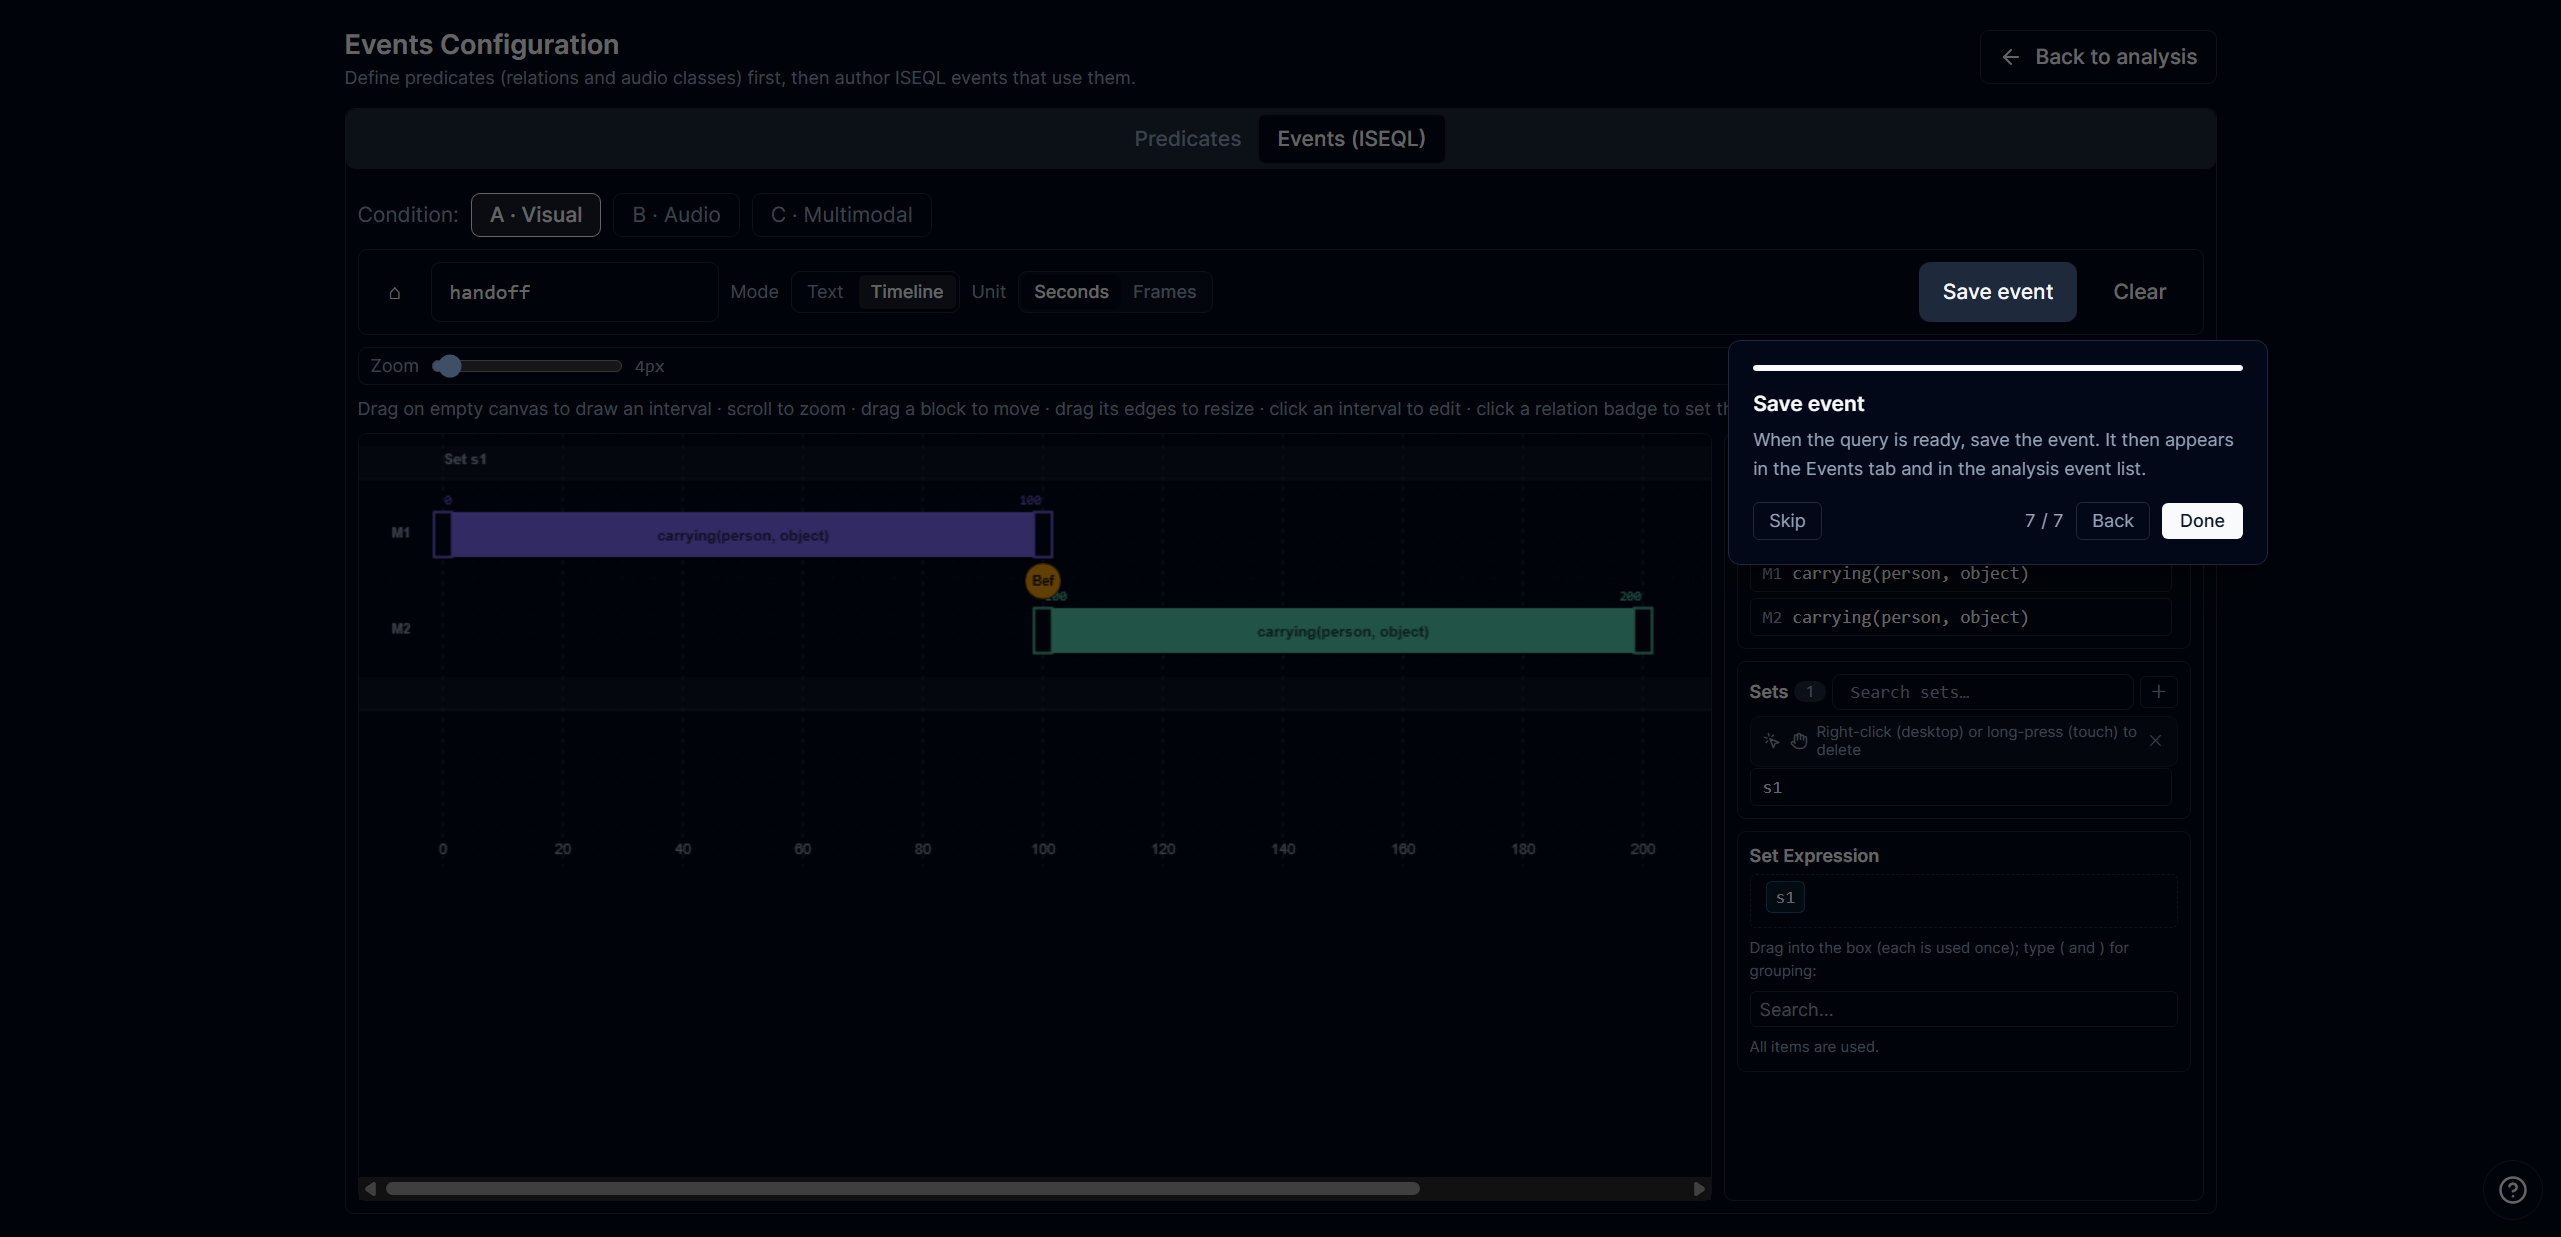
\includegraphics[width=0.92\textwidth]{Figures/appendix/cfg14_timeline_save.png}
  \caption{Save event: when the query is ready, save the event.}
\end{figure}

\section{Visual Only: Handoff}

This example runs condition A (visual only) with the Gemini 3.6 Flash VLM and object re-identification to detect the handoff event. The following figures show the analysis page and the object memory used to maintain consistent object identities.

\begin{figure}[H]
  \centering
  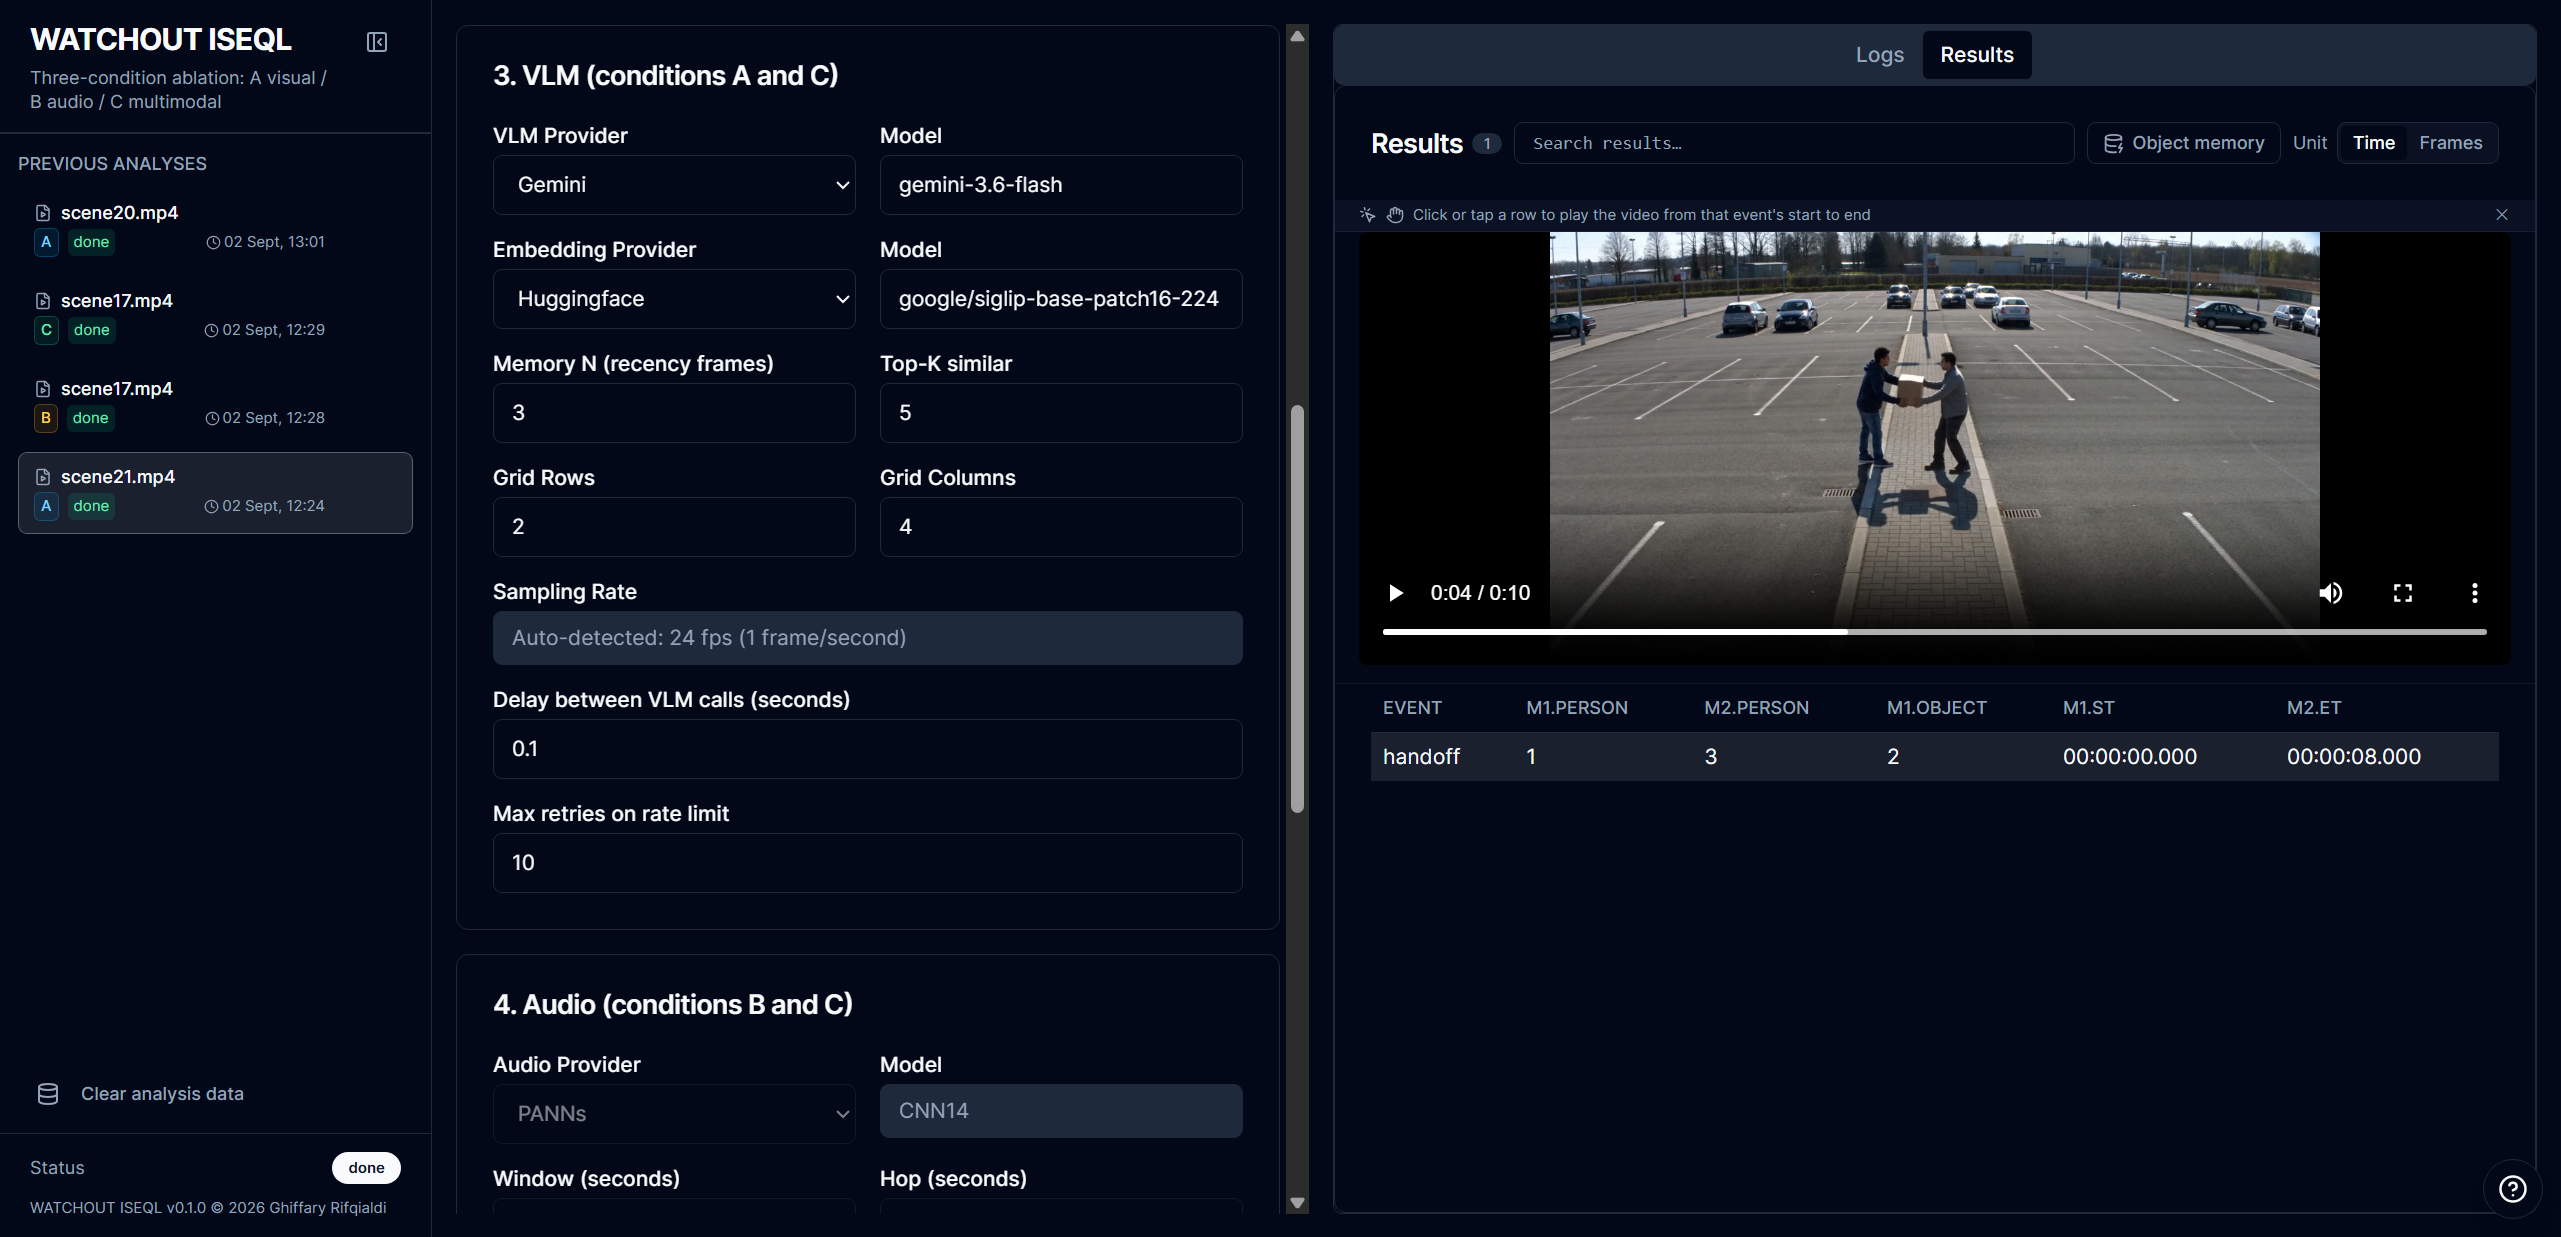
\includegraphics[width=0.92\textwidth]{Figures/appendix/va01_results.png}
  \caption{Visual only (handoff): the results report a handoff detection. The M1.PERSON, M2.PERSON and M1.OBJECT columns hold the persistent identities assigned by re-identification, so the exact people and object involved can be identified.}
\end{figure}

\begin{figure}[H]
  \centering
  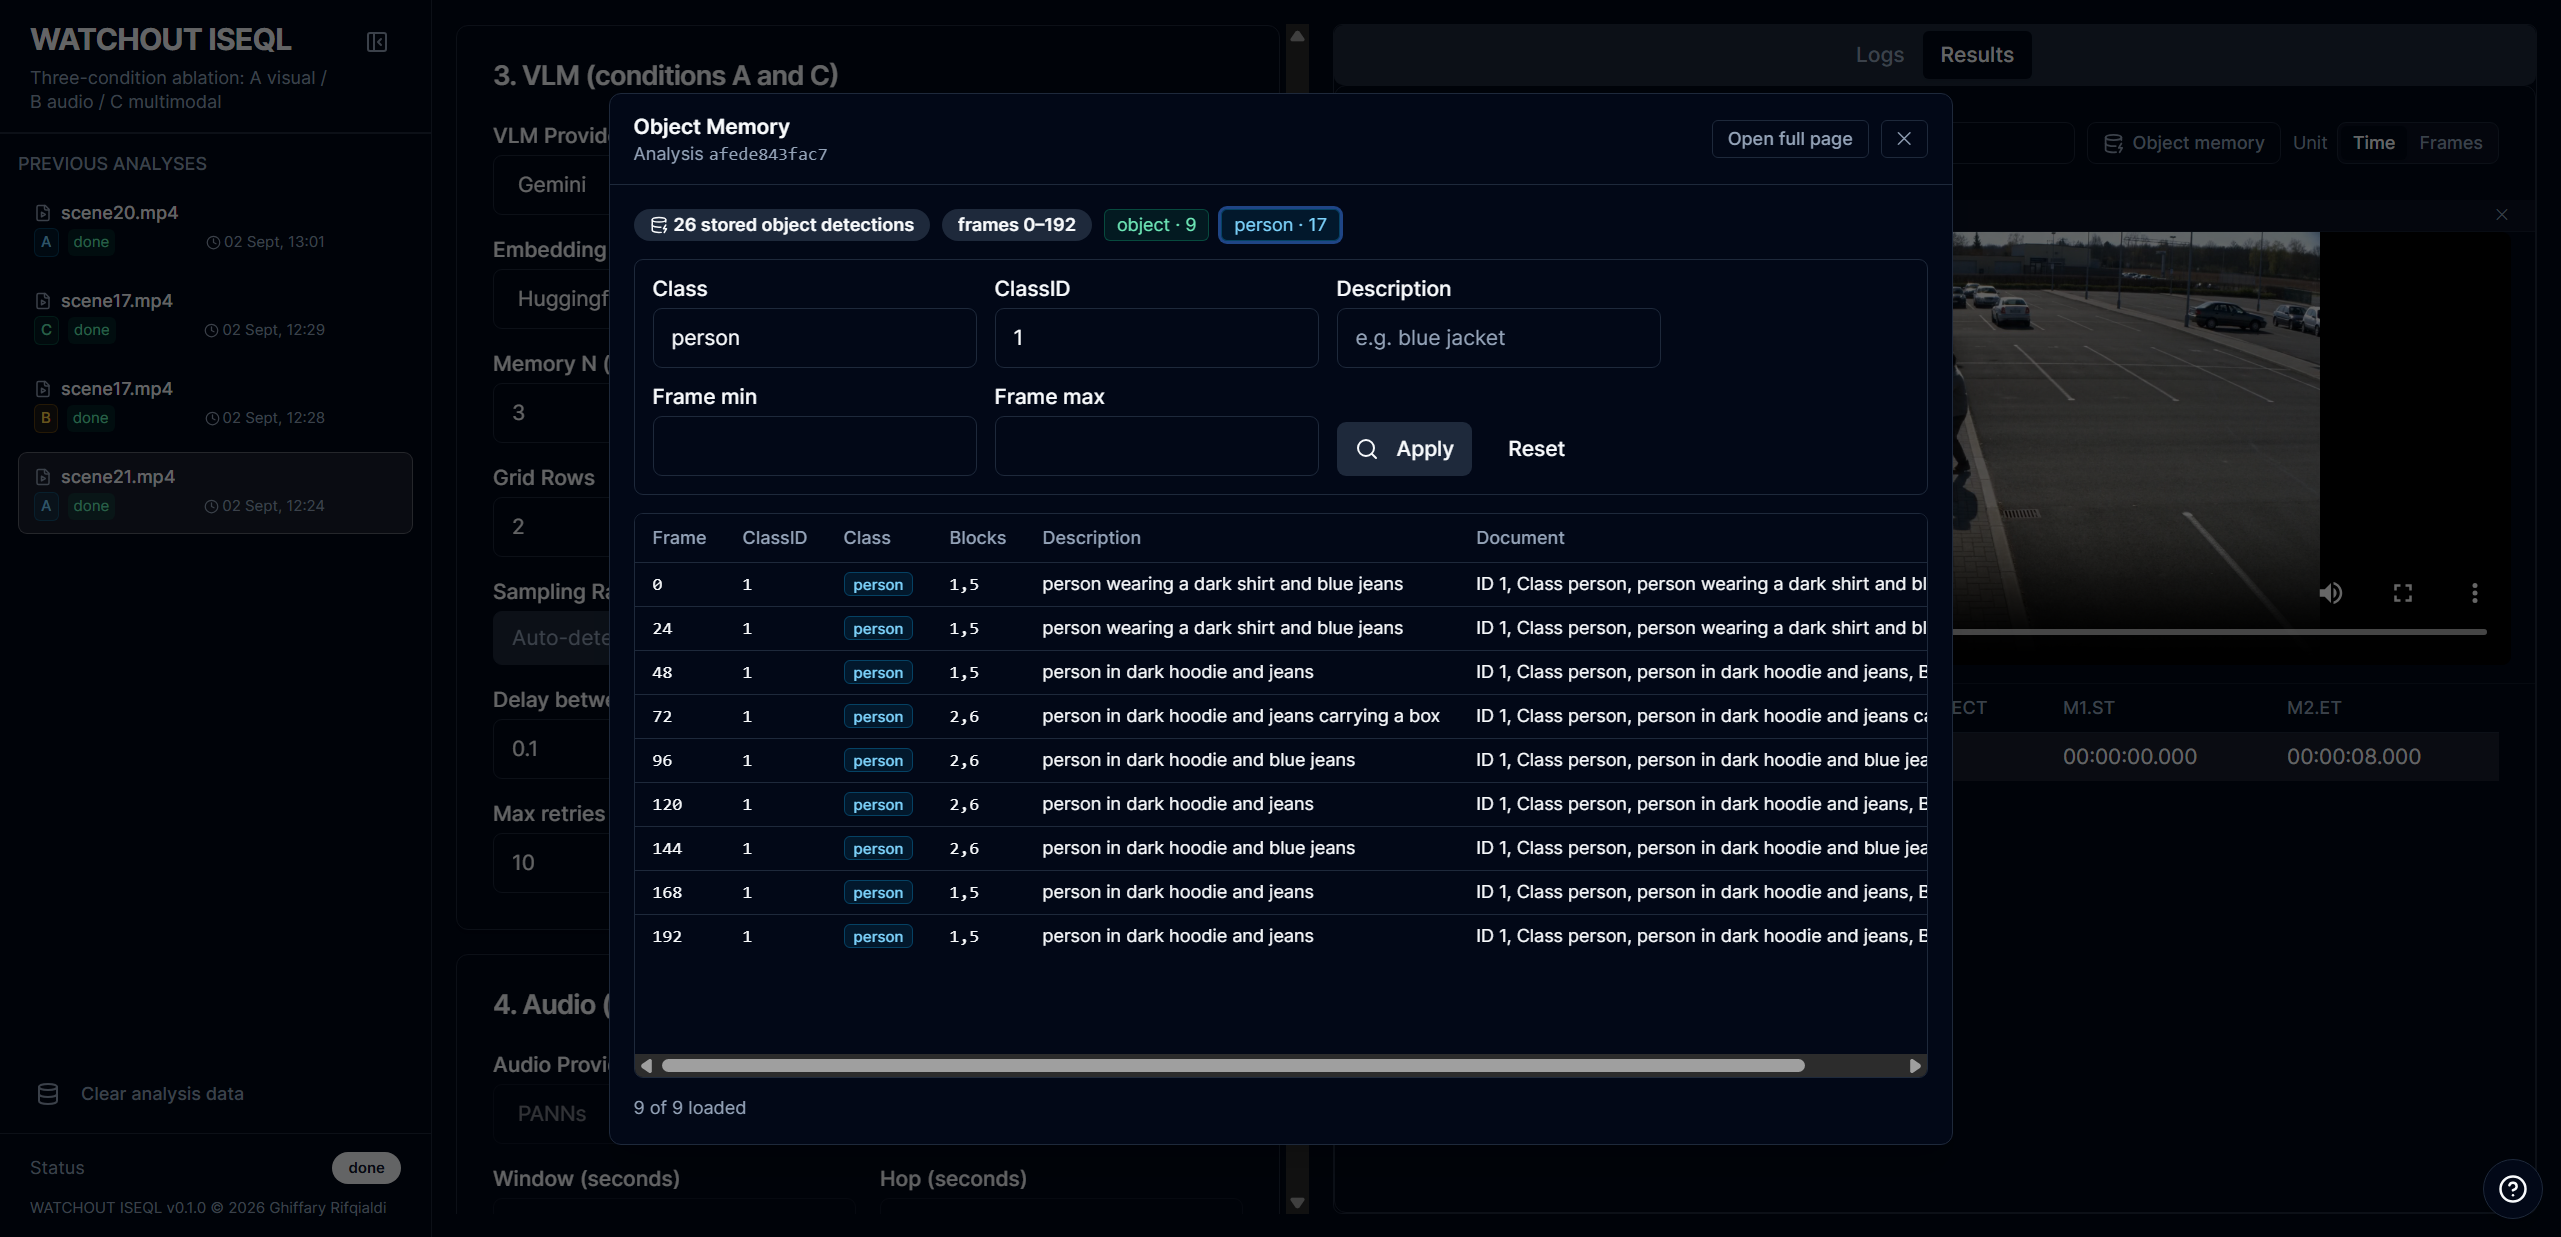
\includegraphics[width=0.92\textwidth]{Figures/appendix/va02_memory_person1.png}
  \caption{Object Memory (visual only, handoff example): person identity 1 (dark shirt); the M1.PERSON column in the result points to this identity, so the person is traceable across the video.}
\end{figure}

\begin{figure}[H]
  \centering
  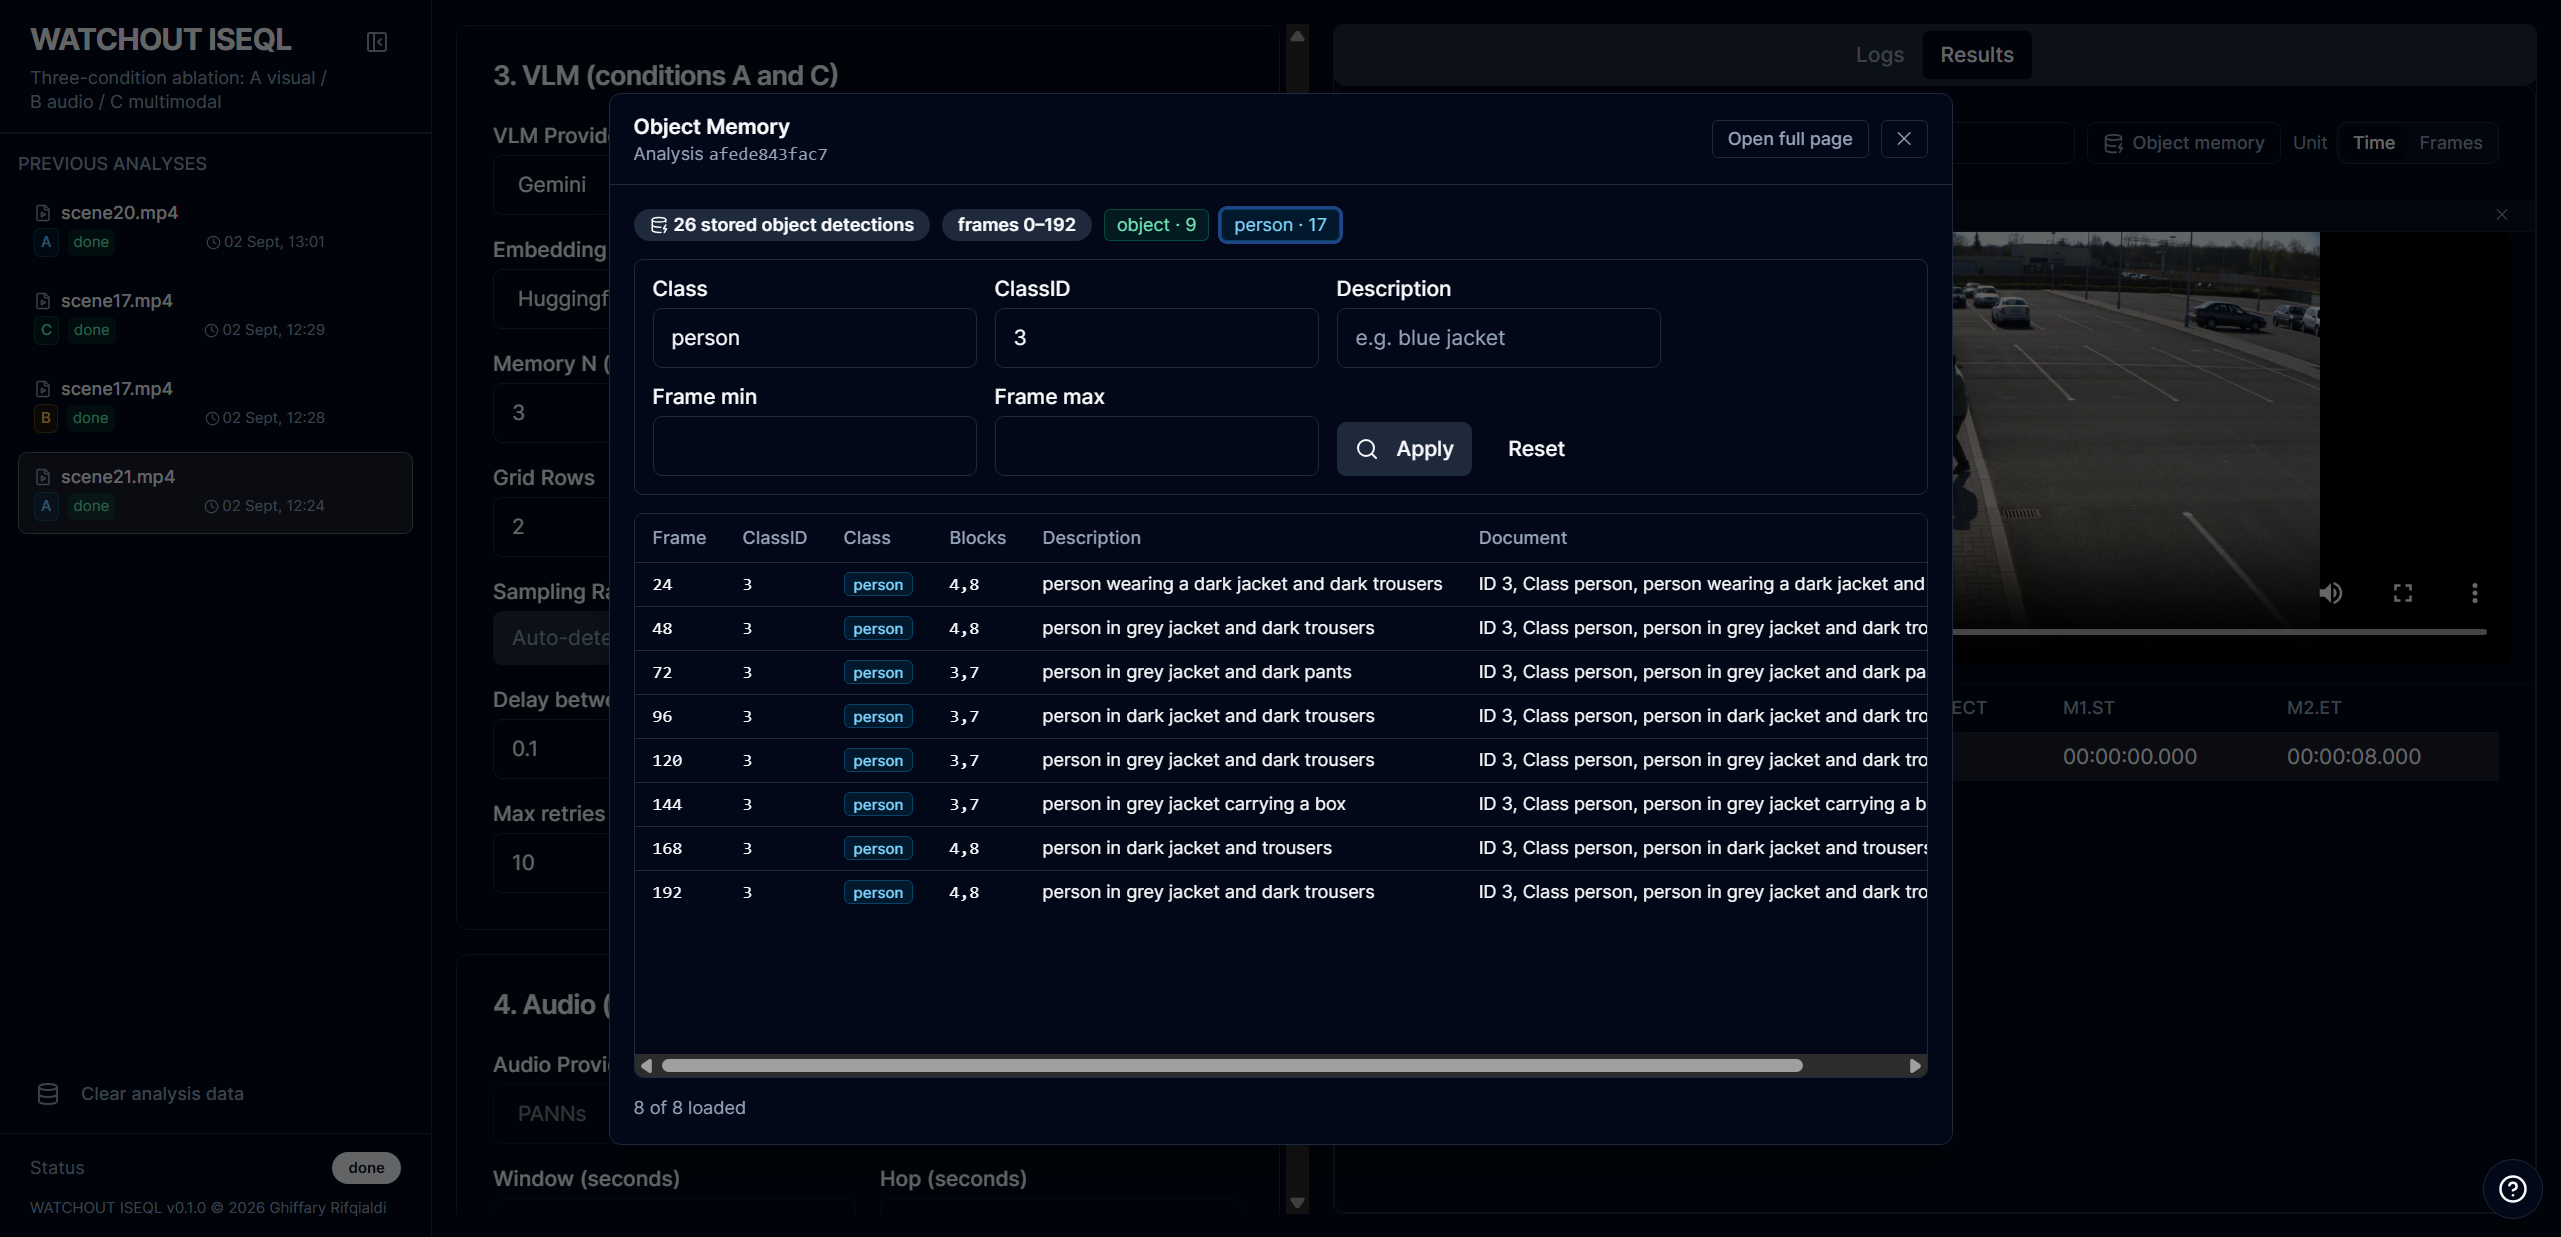
\includegraphics[width=0.92\textwidth]{Figures/appendix/va03_memory_person3.png}
  \caption{Object Memory (visual only, handoff example): person identity 3 (grey jacket); together with identity 1 this shows the handoff passed between two different people.}
\end{figure}

\begin{figure}[H]
  \centering
  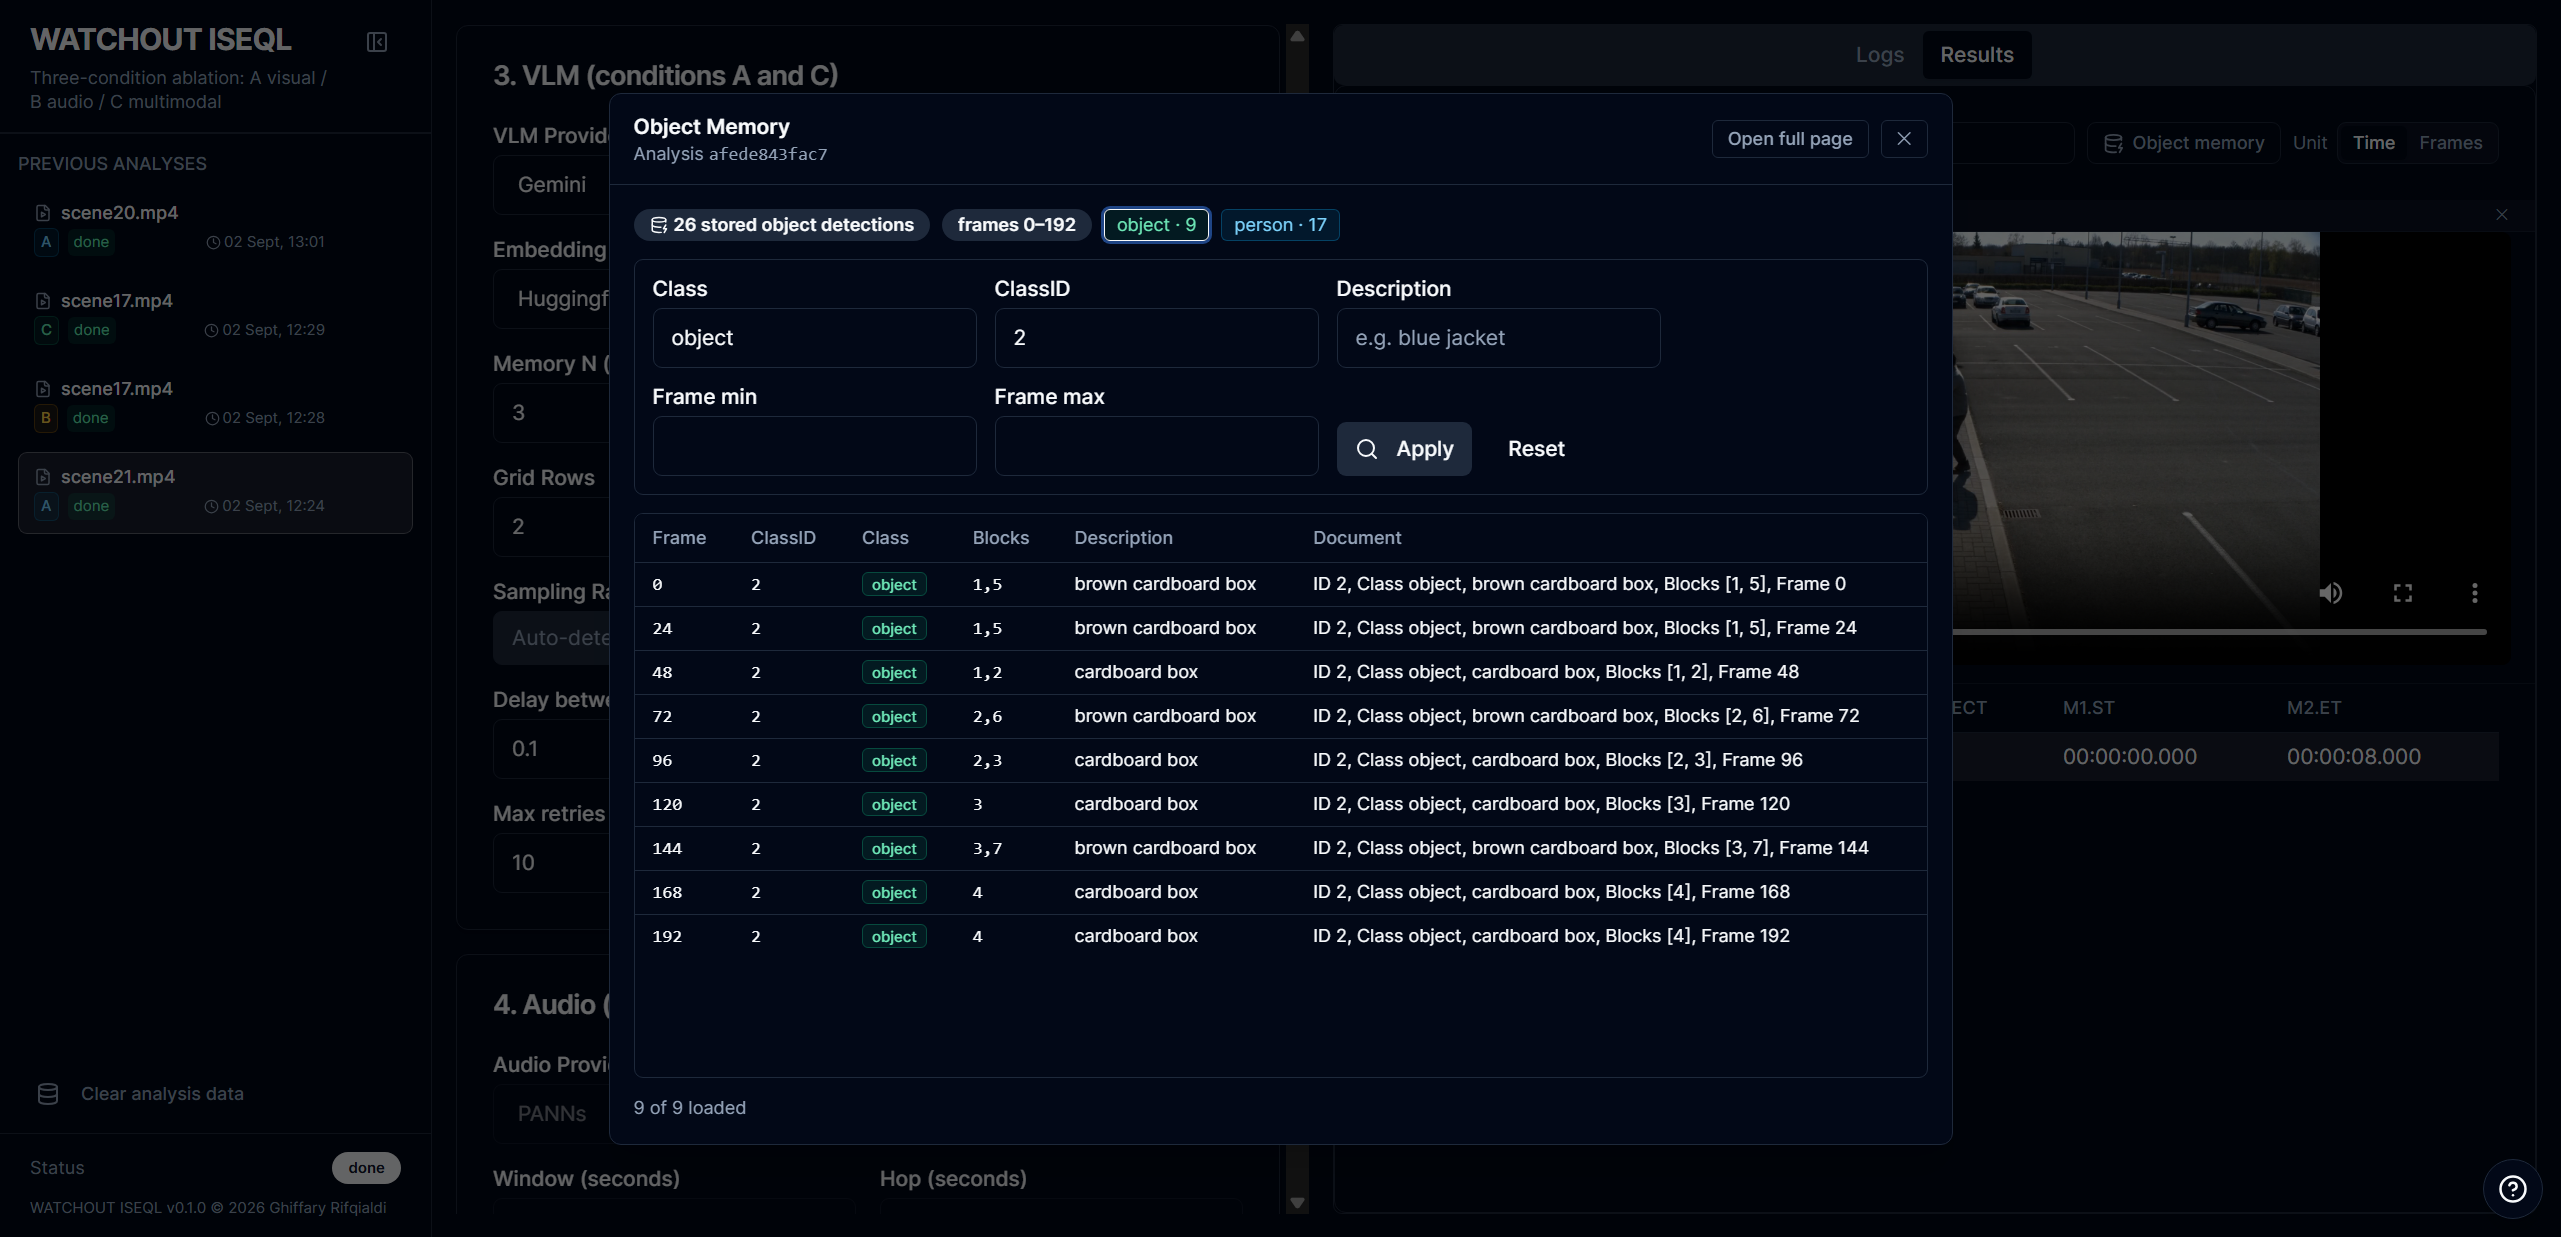
\includegraphics[width=0.92\textwidth]{Figures/appendix/va04_memory_object.png}
  \caption{Object Memory (visual only, handoff example): object identity 2 (brown cardboard box), the carried item referenced by the M1.OBJECT column, which changed hands between the two persons.}
\end{figure}

\section{Audio Only: Vehicle Collision}

This example runs condition B (audio only) through the Qwen2-Audio-7B LALM to detect the vehicle collision event from its audio signature.

\begin{figure}[H]
  \centering
  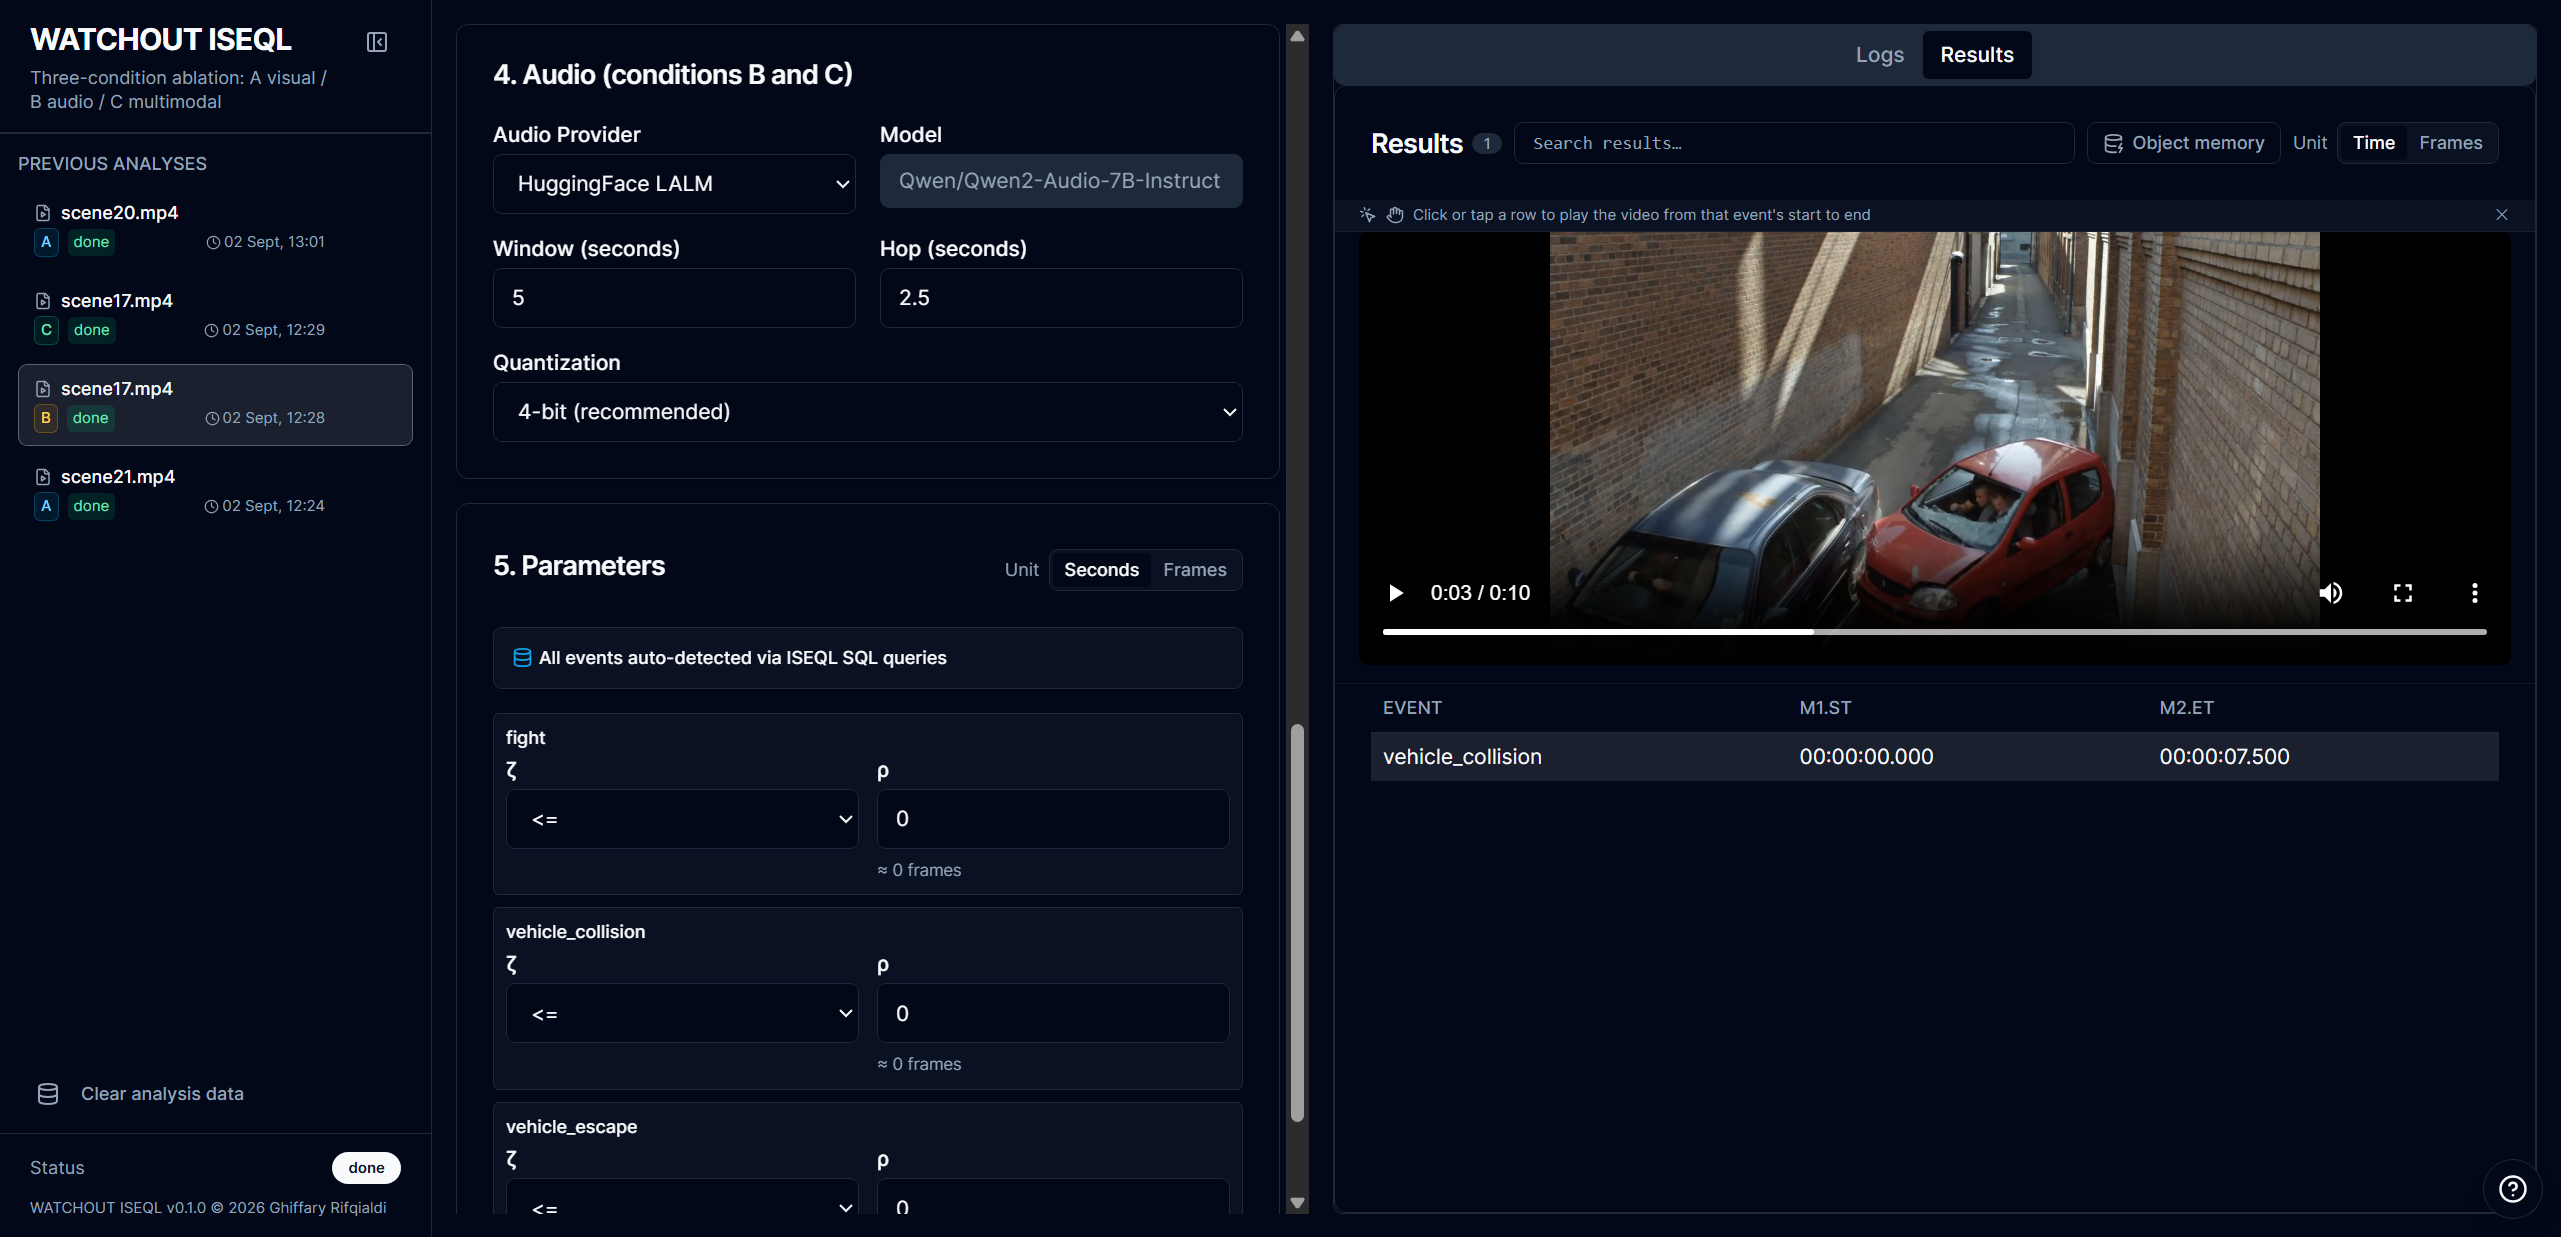
\includegraphics[width=0.92\textwidth]{Figures/appendix/ab01_results.png}
  \caption{Audio only (vehicle collision): the results report the vehicle collision detected from audio, with its start and end timestamps.}
\end{figure}

\section{Multimodal: Vehicle Collision}

This example runs condition C (multimodal), which combines the Gemini 3.6 Flash visual detection and the Qwen2-Audio-7B audio detection via set union, to detect the vehicle collision event using both modalities.

\begin{figure}[H]
  \centering
  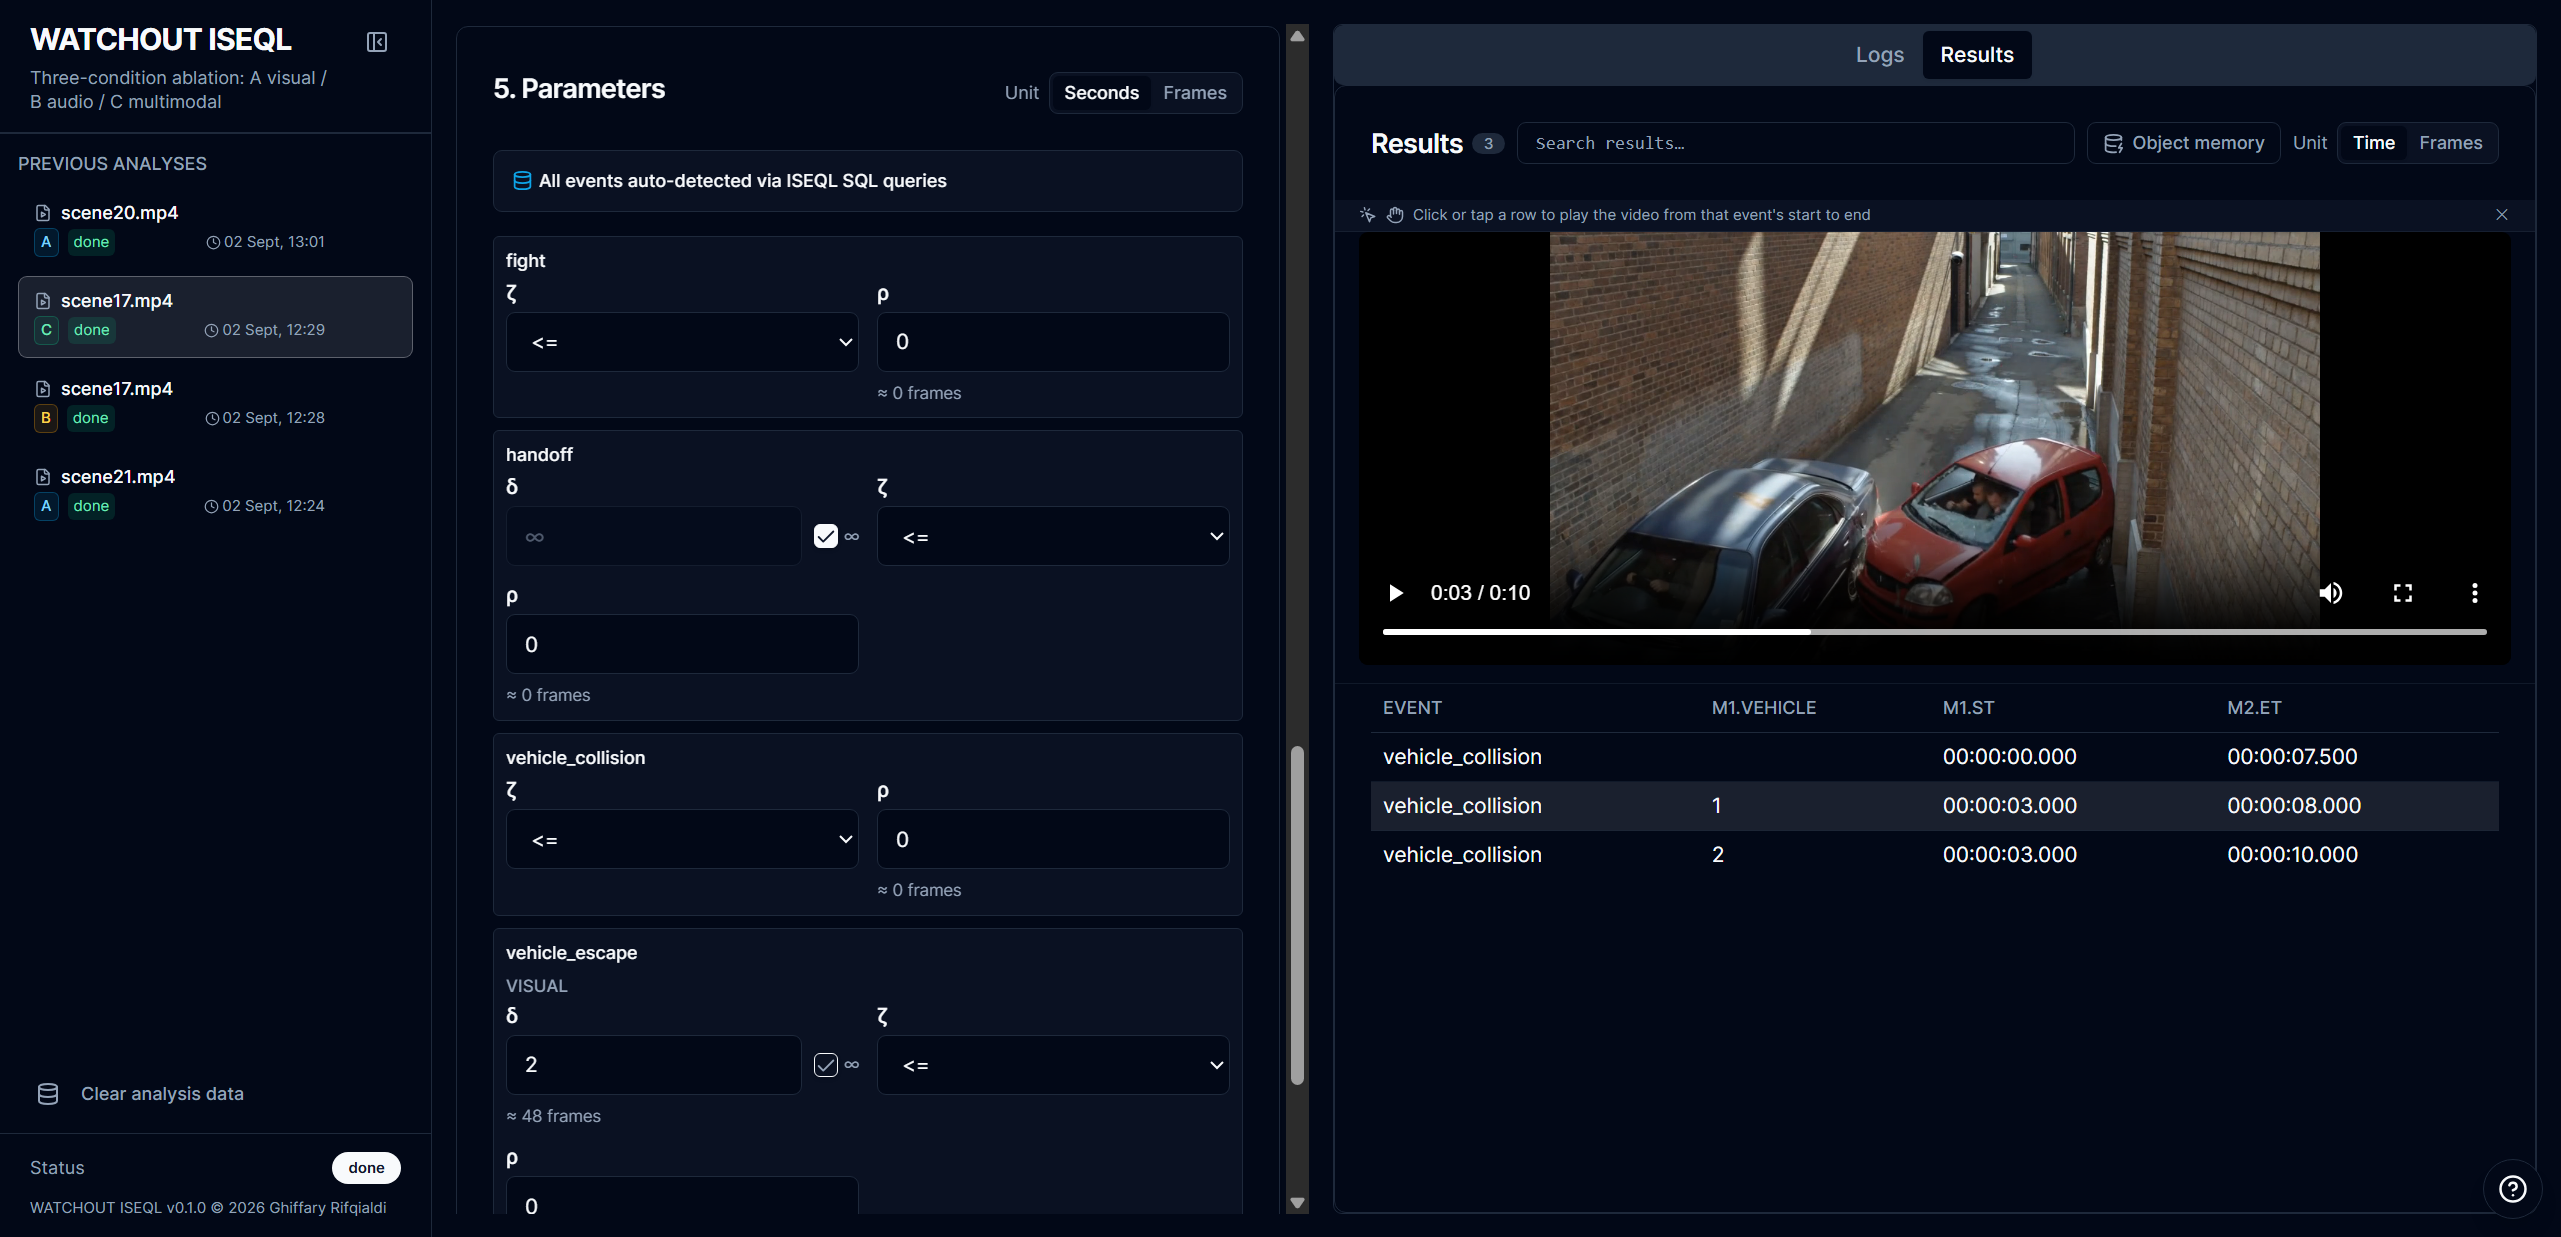
\includegraphics[width=0.92\textwidth]{Figures/appendix/mc01_results.png}
  \caption{Multimodal (vehicle collision): the results list the detected collisions with the M1.VEHICLE identity, so the specific vehicle involved can be identified across frames.}
\end{figure}

\begin{figure}[H]
  \centering
  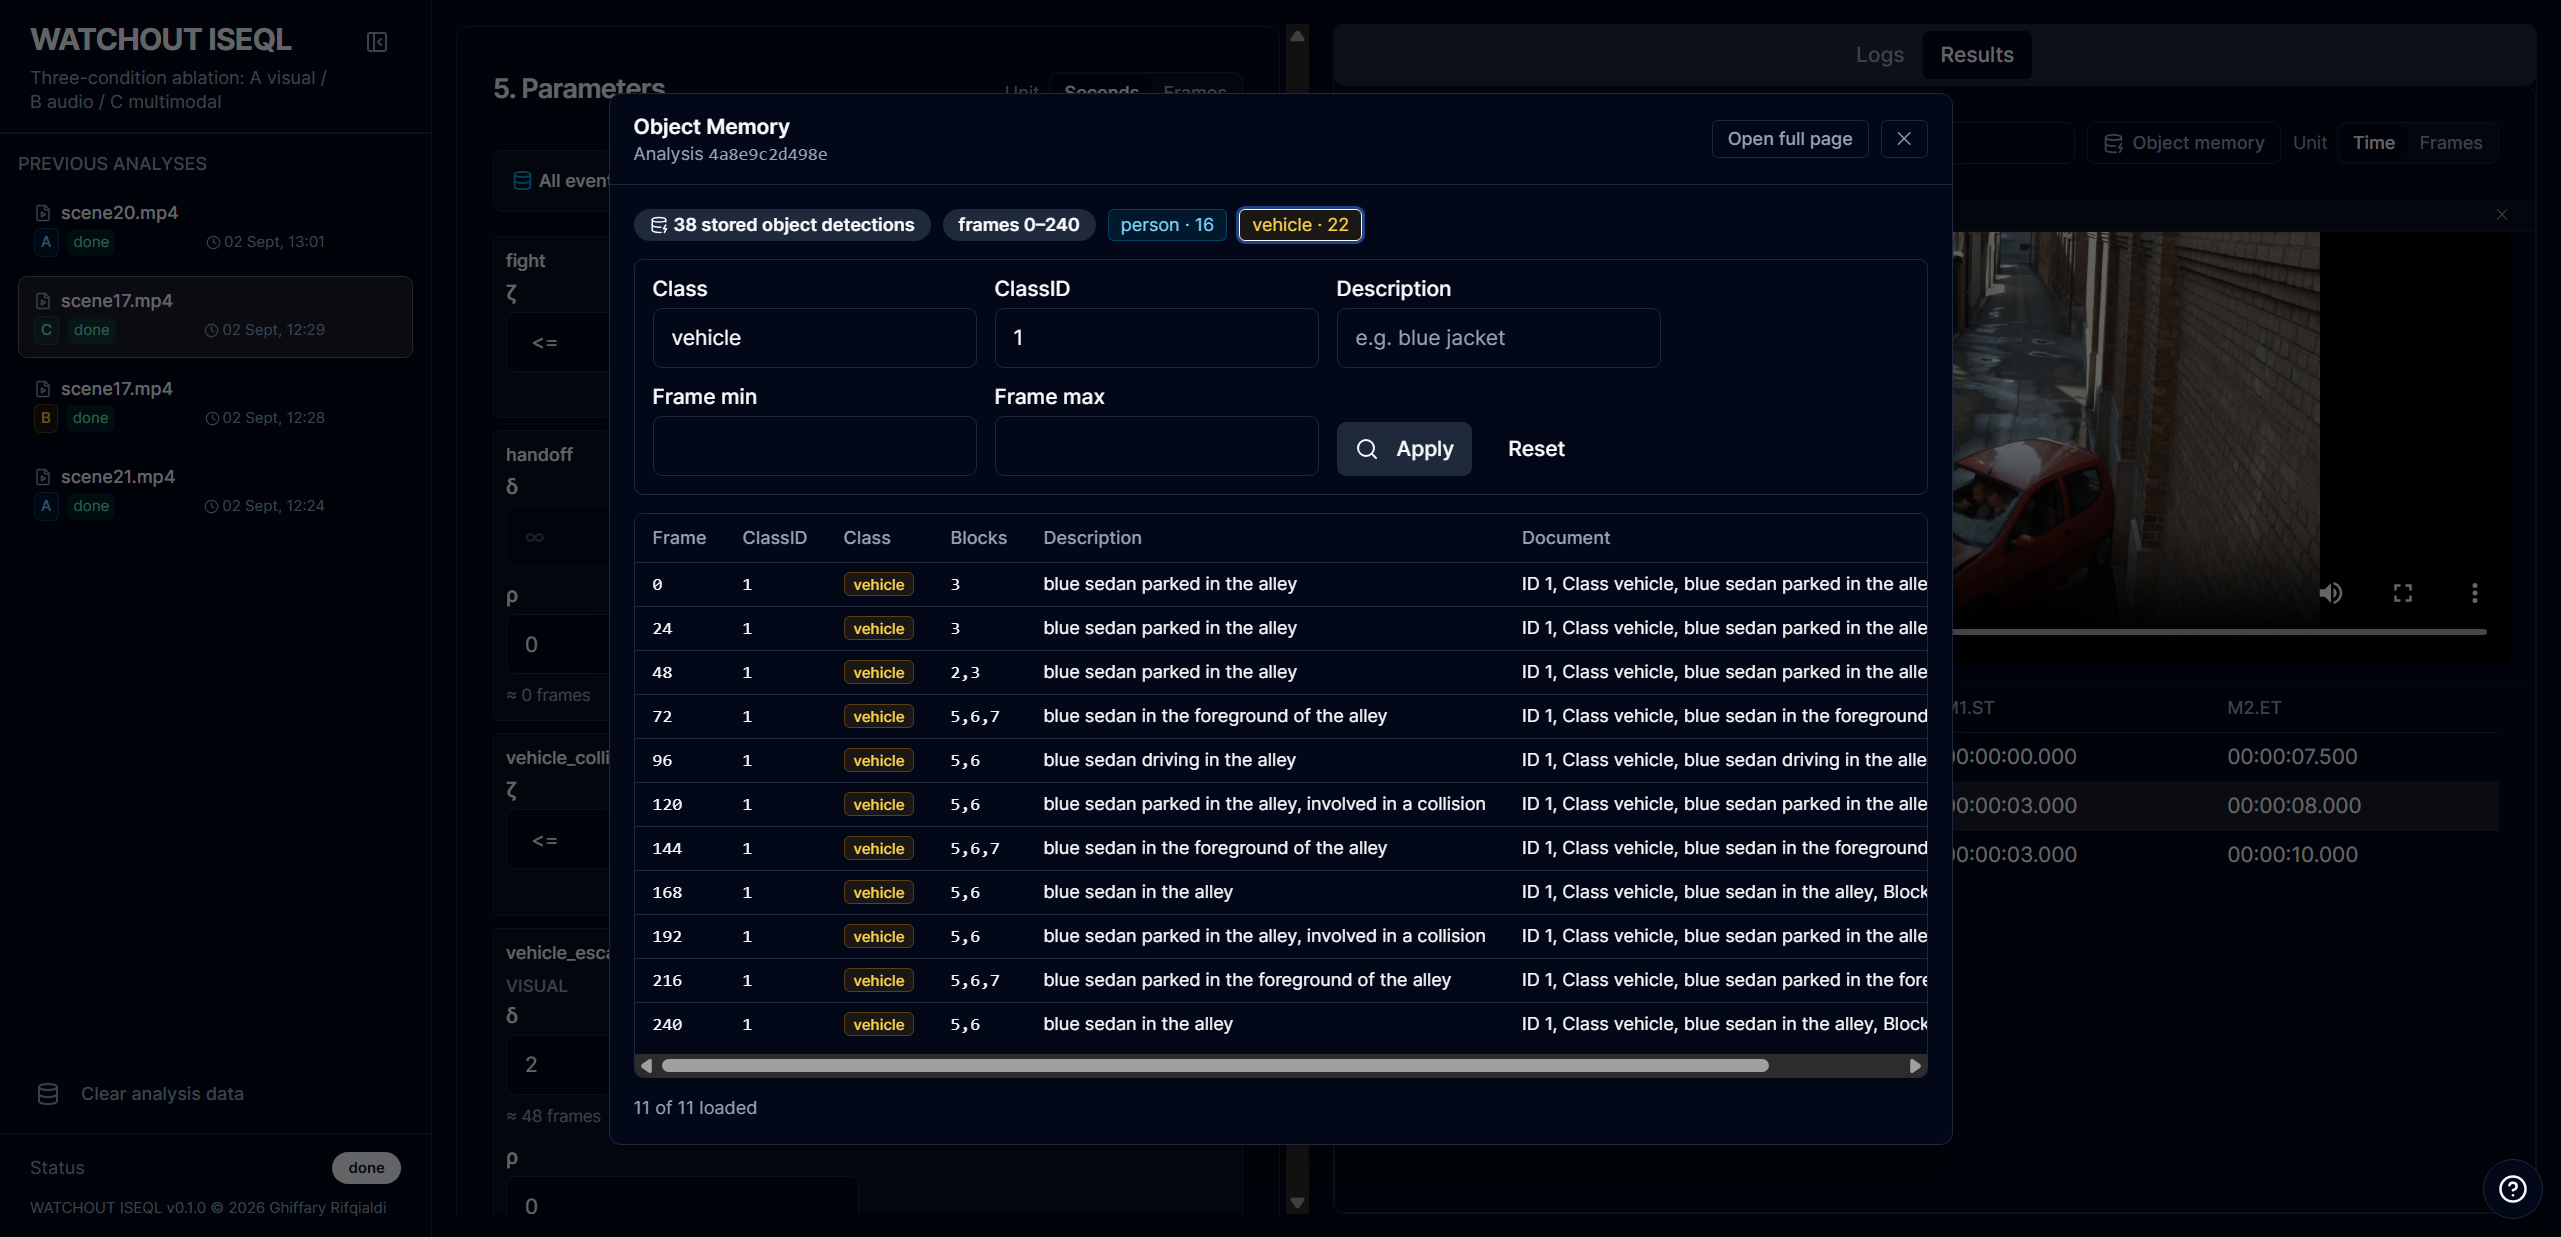
\includegraphics[width=0.92\textwidth]{Figures/appendix/mc02_memory_vehicle1.png}
  \caption{Object Memory (multimodal, vehicle collision example): vehicle identity 1 (red car); the M1.VEHICLE column in the result points to this vehicle.}
\end{figure}

\begin{figure}[H]
  \centering
  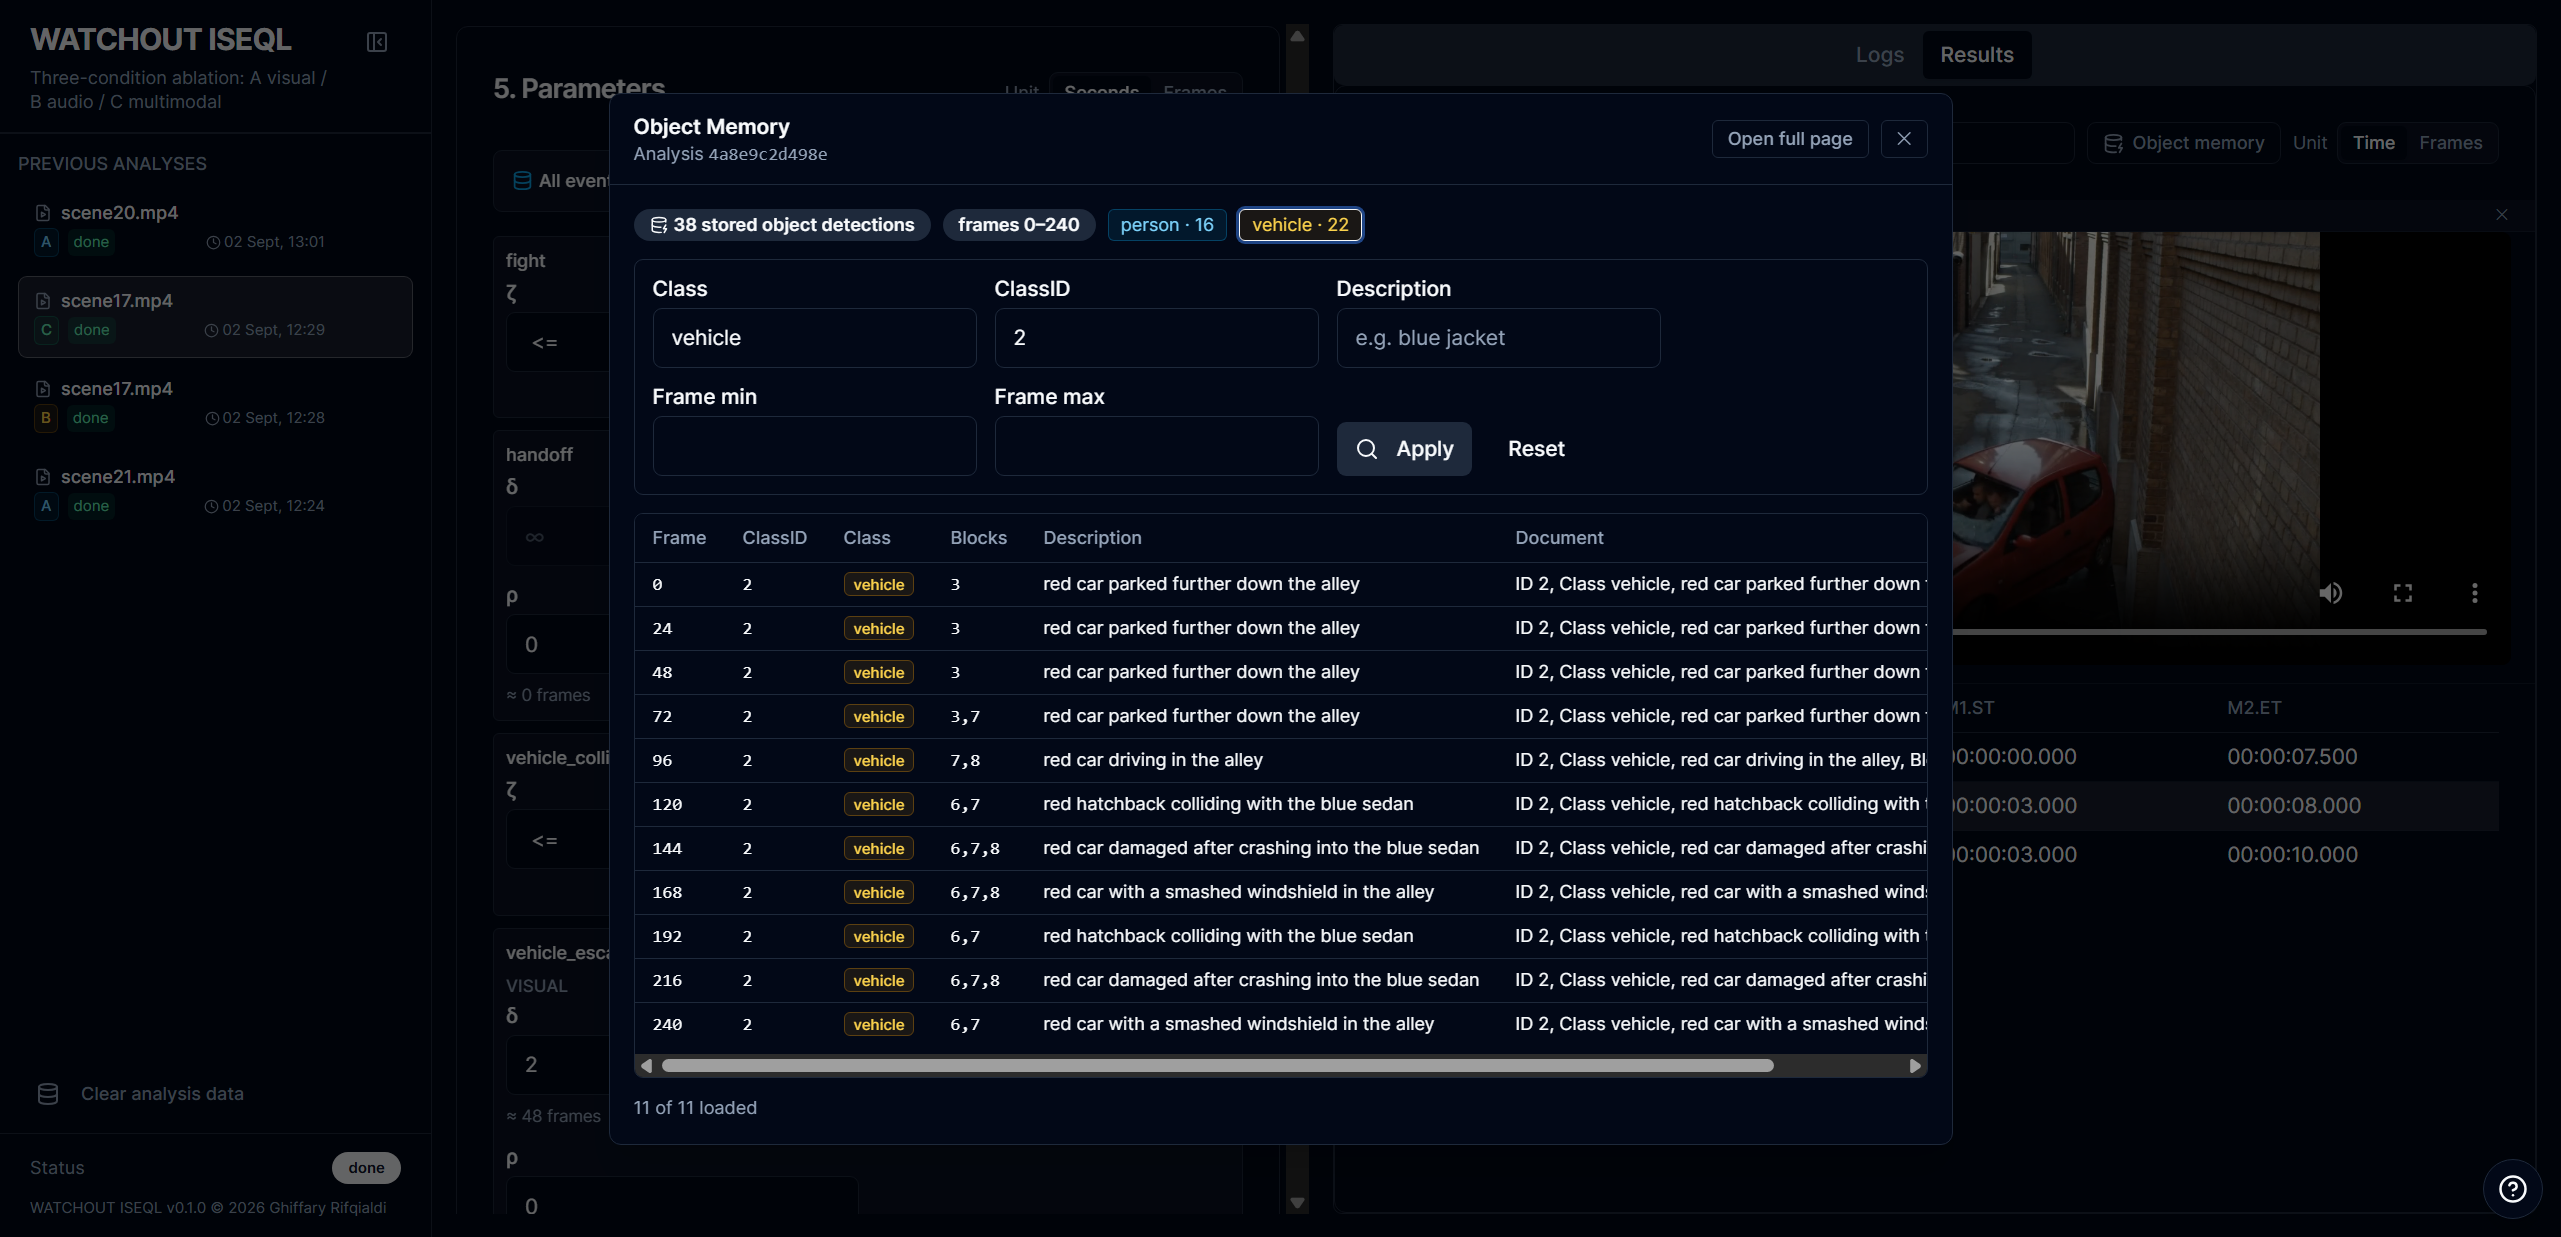
\includegraphics[width=0.92\textwidth]{Figures/appendix/mc03_memory_vehicle2.png}
  \caption{Object Memory (multimodal, vehicle collision example): vehicle identity 2 (a second car); the multimodal union reports both identities as separate detections.}
\end{figure}
